\documentclass[13pt,a4paper]{article}
\usepackage[spanish,es-nodecimaldot]{babel}	% Utilizar español
\usepackage[utf8]{inputenc}					% Caracteres UTF-8
\usepackage{graphicx}						% Imagenes
\usepackage[hidelinks]{hyperref}			% Poner enlaces sin marcarlos en rojo
\usepackage{fancyhdr}						% Modificar encabezados y pies de pagina
\usepackage{float}							% Insertar figuras
\usepackage[textwidth=390pt]{geometry}		% Anchura de la pagina
\usepackage[nottoc]{tocbibind}				% Referencias (no incluir num pagina indice en Indice)
\usepackage{enumitem}						% Permitir enumerate con distintos simbolos
\usepackage[T1]{fontenc}					% Usar textsc en sections
\usepackage{amsmath}						% Símbolos matemáticos
\usepackage[ruled,vlined]{algorithm2e}      % Pseudocódigo
\usepackage{xcolor}
\usepackage{listings}
\usepackage{dsfont}
\usepackage{subfigure}

% Comando para poner el nombre de la asignatura
\newcommand{\asignatura}{Introducción a la Ciencia de Datos}
\newcommand{\autor}{Ignacio Vellido Expósito}
\newcommand{\titulo}{Trabajo teórico/práctico}
\newcommand{\subtitulo}{Análisis de datos, Regresión y Clasificación}

% Configuracion de encabezados y pies de pagina
\pagestyle{fancy}
\lhead{\autor{}}
\rhead{\asignatura{}}
\lfoot{Máster Ciencia de Datos e Ingeniería de Computadores}
\cfoot{}
\rfoot{\thepage}
\renewcommand{\headrulewidth}{0.4pt}		% Linea cabeza de pagina
\renewcommand{\footrulewidth}{0.4pt}		% Linea pie de pagina

% ==============================================================================
% ==============================================================================

\usepackage{booktabs}
\usepackage{longtable}
\usepackage{array}
\usepackage{multirow}
\usepackage{wrapfig}
\usepackage{float}
\usepackage{colortbl}
\usepackage{pdflscape}
\usepackage{tabu}
\usepackage{threeparttable}
\usepackage{threeparttablex}
\usepackage[normalem]{ulem}
\usepackage{makecell}
\usepackage{xcolor}

% ==============================================================================
% ==============================================================================

\begin{document}
    \pagenumbering{gobble}
    % ==============================================================================
% Pagina de titulo
\begin{titlepage}
    \begin{minipage}{\textwidth}
        \centering

        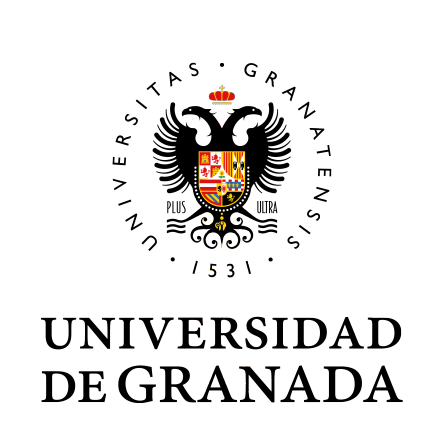
\includegraphics[scale=0.5]{img/ugr.png}\\

        \textsc{\Large \asignatura{}\\[0.2cm]}
        \textsc{MÁSTER CIENCIA DE DATOS E INGENIERÍA DE COMPUTADORES}\\[1cm]

        \noindent\rule[-1ex]{\textwidth}{1pt}\\[1.5ex]
        \textsc{{\Huge \titulo\\[0.5ex]}}
        \textsc{{\Large \subtitulo\\}}
        \noindent\rule[-1ex]{\textwidth}{2pt}\\[2.5ex]

        \end{minipage}

        \vspace{0.3cm}

        \begin{minipage}{\textwidth}

        \centering

        \textbf{Autor}\\ {\autor{} \\ ignaciove@correo.ugr.es}\\[1.5ex]
        \vspace{0.4cm}

        
\includegraphics[scale=0.3]{img/etsiit.jpeg}
        
\includegraphics[scale=0.6]{img/master.png}

        \vspace{0.7cm}
        \textsc{Escuela Técnica Superior de Ingenierías Informática y de Telecomunicación}\\
        \vspace{1cm}
        \textsc{Curso 2020-2021}
    \end{minipage}
\end{titlepage}
% ==============================================================================
    
    \pagenumbering{arabic}
    \tableofcontents
    \thispagestyle{empty}				% No usar estilo en la pagina de indice

    \newpage

    % ==============================================================================

    % \section{Introducción} \newpage
    \section{Regresión: Análisis Estadístico de Datos}

\subsection{Introducción}

Para el problema de regresión hacemos uso del dataset \textbf{autoMPG6} \cite{autompg}, donde se codifica el consumo de gasolina de distintos coches (en millas por galón, Mpg) en base a las siguientes características:

\begin{enumerate}
\def\labelenumi{\arabic{enumi}.}
    \item \textbf{Displacement}: Indica la cilindrada del coche, la suma del volumen útil de los cilindros del motor, medido en pulgadas cúbicas.
    \item \textbf{Horse\_power}: Mide la potencia del coche.
    \item \textbf{Weight}: Peso en libras.
    \item \textbf{Acceleration}: Aceleración del coche de 0 a 60 millas por hora, medido
    en segundos.
    \item \textbf{Model\_year}: Indica las dos últimas cifras del año de producción.
\end{enumerate}

El objetivo es poder predecir con estos cinco atributos el consumo de Mpg de un nuevo coche:

\begin{enumerate}
    \def\labelenumi{\arabic{enumi}.}
    \setcounter{enumi}{5}
    \item \textbf{Mpg}: Millas-por-galón, indica la cantidad de galones (1G $\approx$ 3,78L) de fuél que consume un vehículo al recorrer una milla (1m $\approx$ 1,6km).
\end{enumerate}

El dataset contiene 392 instancias codificando esta información.

\vspace{\baselineskip}

La descripción del problema nos da alguna información adicional sobre las variables:

\begin{enumerate}
    \def\labelenumi{\arabic{enumi}.}
    \item \textbf{Displacement}: Variable numérica continua, contamos con valores reales en el rango {[}68.0,455.0{]}.
    \item \textbf{Horse\_power}: Variable numérica continua, contamos con valores enteros en el rango {[}46,230{]}.
    \item \textbf{Weight}: Variable numérica continua, contamos con valores enteros en el rango {[}1613,5140{]}.
    \item \textbf{Acceleration}: Variable numérica continua, contamos con valores reales en el rango {[}8.0,24.8{]}.
    \item \textbf{Model\_year}: Variable numérica discreta, contamos con valores enteros en el rango {[}70,82{]}.
    \item \textbf{Mpg}: Variable numérica continua, contamos con valores reales en el rango {[}9.0,46.6{]}.
\end{enumerate}

\paragraph{Hipótesis de partida}

\begin{itemize}
    \item \textbf{H.1}: Horse\_power puede influir en Mpg: A más potencia, más consumo.
    \item \textbf{H.2}: Weight debe influir en Mpg: Un coche más pesado debería consumir más.
    \item \textbf{H.3}: Debería haber correlación entre displacement (cilindrada) con horse y acceleration
    \item \textbf{H.4}: Horse y acceleration podrían estar relacionadas
    \item \textbf{H.5}: Viendo que contamos con un rango pequeño de años, no debería haber un cambio significativo de prestaciones entre años
    \item \textbf{H.6}: Pero debería existir una tendencia de mejora de prestaciones con los años, incluyendo aumento de Displacement, Horse\_power y Acceleration.
    \item \textbf{H.7}: Model\_year podría no mostrar relación con Mpg: Pese al paso de los años si contamos con diferentes tipos de vehículos (todoterrenos, familiares, deportivos\ldots) podría haber un consumo dispar. (Si existiera tendencia, viendo que los años son de las últimas décadas del siglo XX, podría ir el consumo hacia abajo)
    \item \textbf{H.8}: Esta última hipótesis se puede aplicar al resto de variables, indicándonos que Model\_year no debería tener relevancia para este problema de regresión.
    \item \textbf{H.9}: Horse\_power podría depender de las variables Displacement y Weight
\end{itemize}

\subsection{Análisis Estadístico de Datos}

Antes de comenzar a analizar las variables nos plantemos una cuestión: ¿Debemos considerar Model\_year como una variable numérica o como un factor categórico? Aunque por la hipótesis H.7 podríamos acabar no eligiendo la variable para el problema, es necesario preguntarnos por esto antes de comenzar.

\vspace{\baselineskip}

Sabemos que las observaciones para esta variable cuenta con valores entre 72 y 82, por lo que tenemos información exacta del año (en comparación, por ejemplo, con agrupaciones mayores como la década o el siglo). El hecho de tratarla como categórica o cuantitativa depende mucho del problema. En este caso, tenemos interés en cuestionarnos por valores entre años, por ejemplo, el consumo entre los años 75 y 76.

\vspace{\baselineskip}

Por tanto, de cara al problema de regresión que nos atañe, tendríamos dos opciones: 
\begin{itemize}
    \item Mantenerlo como categórico y generar variables dummy (valores 0-1 para indicar si la instancia es de ese año). Suponiendo que tenemos al menos una instancia de cada año, esto nos generaría 12 variables nuevas. 
    \item Mantenerlo como numérico, pero teniendo cuidado de cómo interpretar el año.
\end{itemize}

\vspace{\baselineskip}

Proseguimos con tanto dejando Model\_year como variable numérica.

\subsubsection{Análisis univariable}
  
La cabecera de nuestro dataset tiene esta forma:

\vspace{\baselineskip}

\begin{tabular}{|r|r|r|r|r|r|}
    \hline
    Displacement & Horse\_power & Weight & Acceleration & Model\_year & Mpg\\
    \hline
    91 & 70 & 1955 & 20.5 & 71 & 26.0\\
    \hline
    232 & 100 & 2789 & 15.0 & 73 & 18.0\\
    \hline
    350 & 145 & 4055 & 12.0 & 76 & 13.0\\
    \hline
    318 & 140 & 4080 & 13.7 & 78 & 17.5\\
    \hline
    113 & 95 & 2372 & 15.0 & 70 & 24.0\\
    \hline
    97 & 60 & 1834 & 19.0 & 71 & 27.0\\
    \hline
\end{tabular}

\vspace{\baselineskip}

Y con la siguiente información estadística:

\begin{verbatim}
  Displacement    Horse_power        Weight      Acceleration     Model_year   
 Min.   : 68.0   Min.   : 46.0   Min.   :1613   Min.   : 8.00   Min.   :70.00  
 1st Qu.:105.0   1st Qu.: 75.0   1st Qu.:2225   1st Qu.:13.78   1st Qu.:73.00  
 Median :151.0   Median : 93.5   Median :2804   Median :15.50   Median :76.00  
 Mean   :194.4   Mean   :104.5   Mean   :2978   Mean   :15.54   Mean   :75.98  
 3rd Qu.:275.8   3rd Qu.:126.0   3rd Qu.:3615   3rd Qu.:17.02   3rd Qu.:79.00  
 Max.   :455.0   Max.   :230.0   Max.   :5140   Max.   :24.80   Max.   :82.00  
      Mpg       
 Min.   : 9.00  
 1st Qu.:17.00  
 Median :22.75  
 Mean   :23.45  
 3rd Qu.:29.00  
 Max.   :46.60  
\end{verbatim}

\vspace{\baselineskip}

El dataset \textbf{no} cuenta con \textbf{valores repetidos} ni \textbf{missing values}.

\vspace{\baselineskip}

Mostramos scatterplots univariables:
\begin{figure}[H]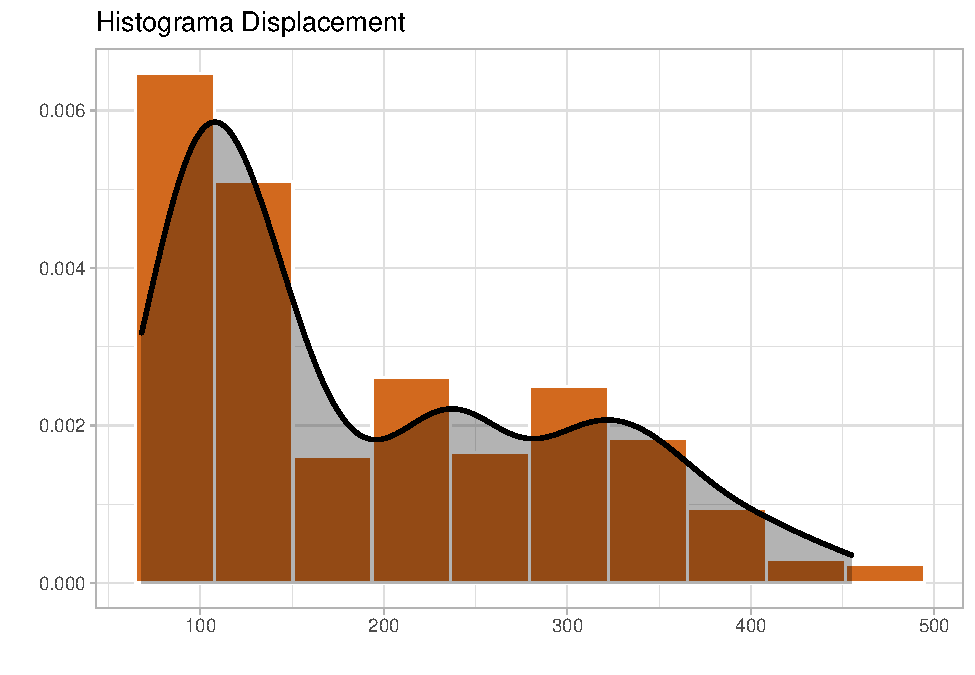
\includegraphics[width=.9\linewidth]{img/EDA_files/figure-latex/unnamed-chunk-7-1}\caption{}\end{figure}
\begin{figure}[H]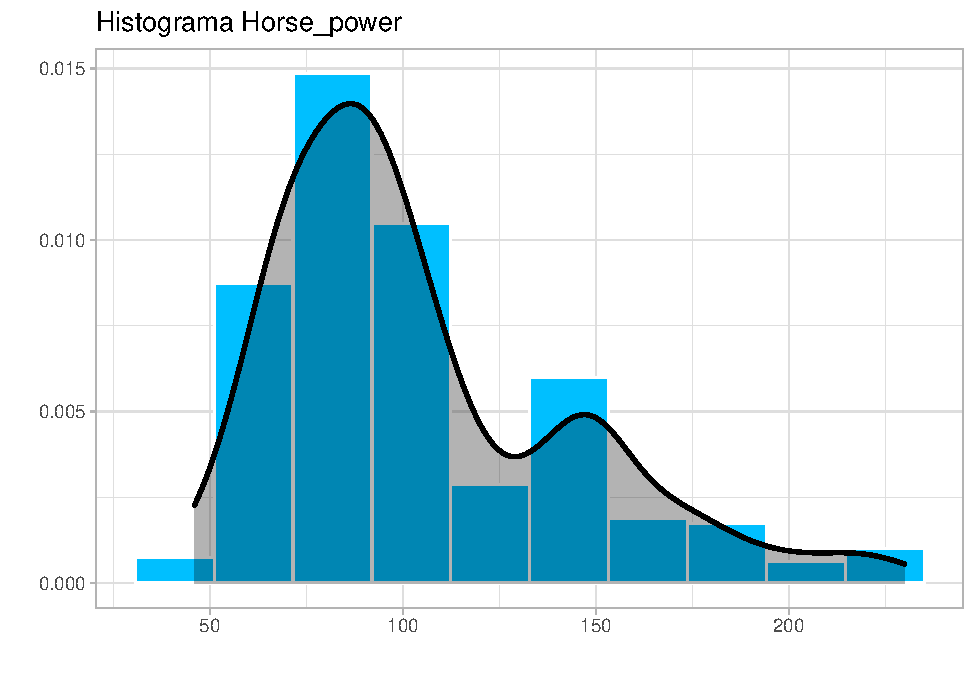
\includegraphics[width=.9\linewidth]{img/EDA_files/figure-latex/unnamed-chunk-7-2} \caption{}\end{figure}
\begin{figure}[H]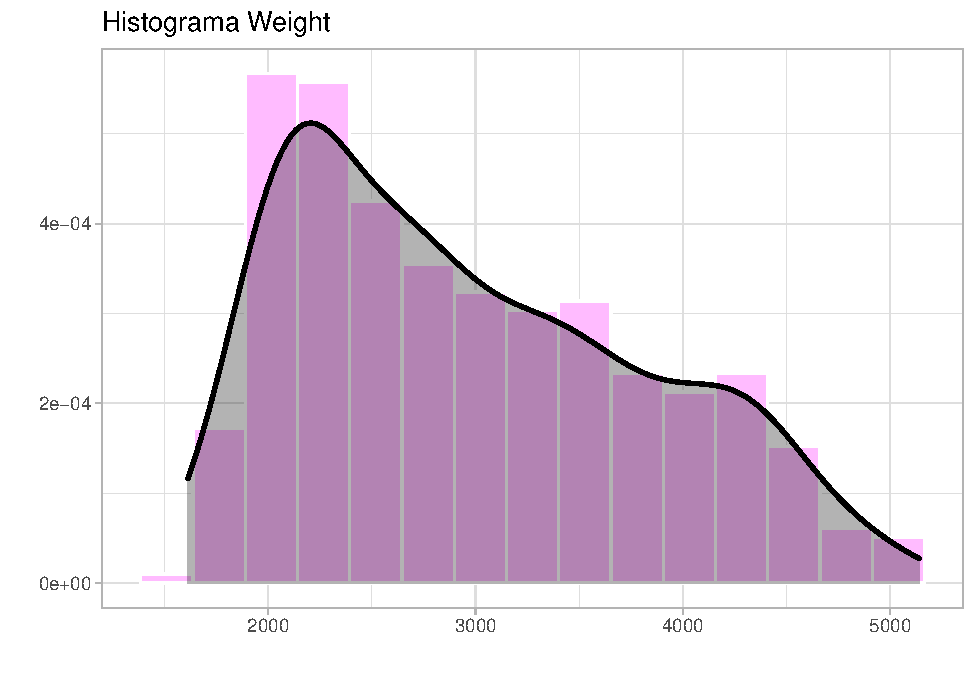
\includegraphics[width=.9\linewidth]{img/EDA_files/figure-latex/unnamed-chunk-7-3} \caption{}\end{figure}
\begin{figure}[H]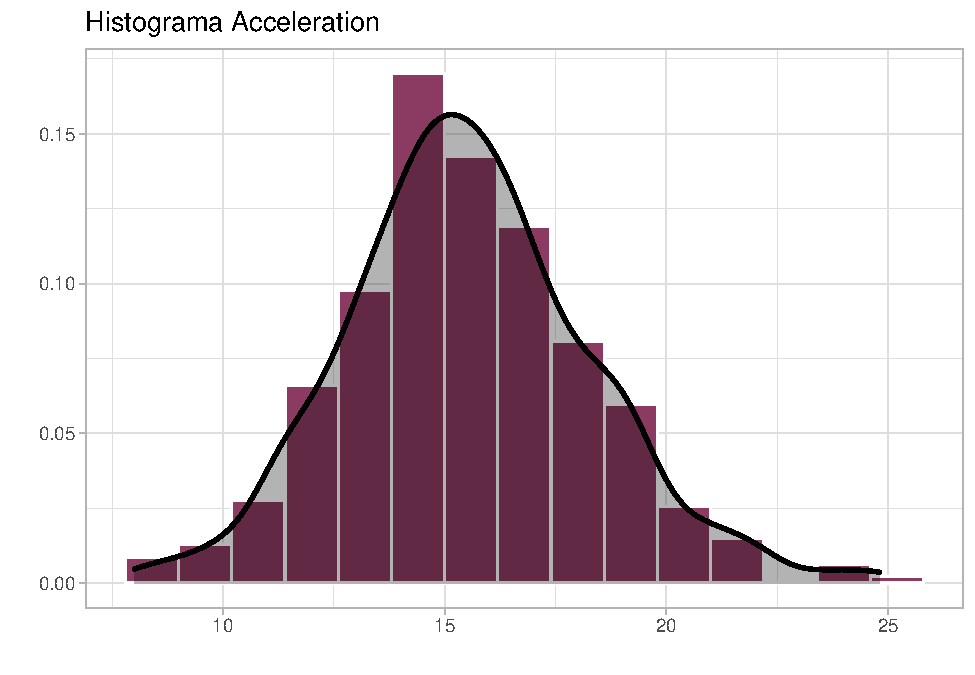
\includegraphics[width=.9\linewidth]{img/EDA_files/figure-latex/unnamed-chunk-7-4} \caption{}\end{figure}
\begin{figure}[H]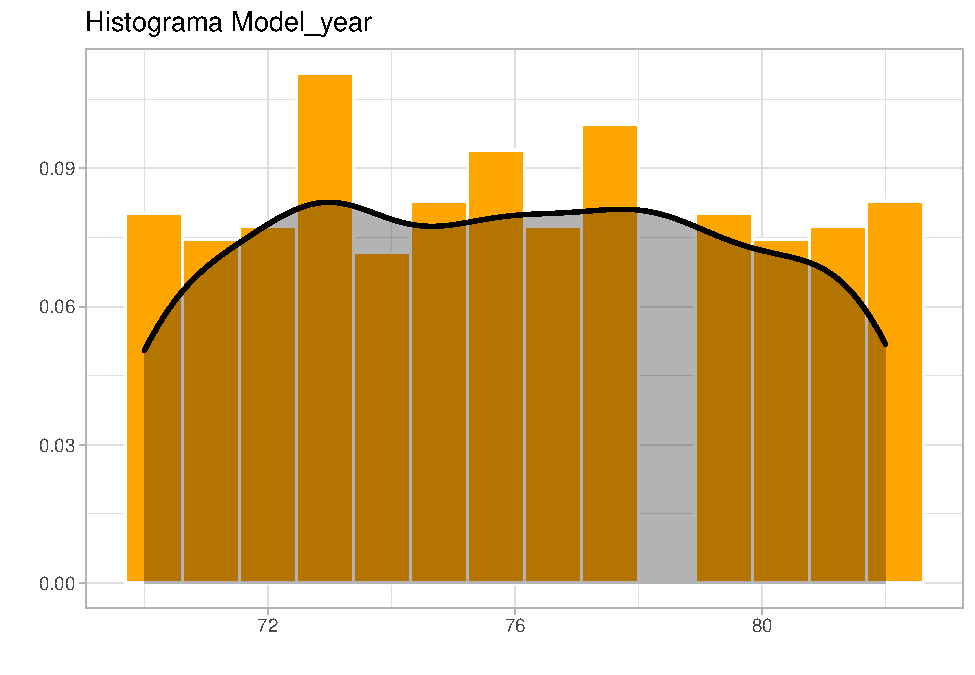
\includegraphics[width=.9\linewidth]{img/EDA_files/figure-latex/unnamed-chunk-7-5} \caption{}\end{figure}
\begin{figure}[H]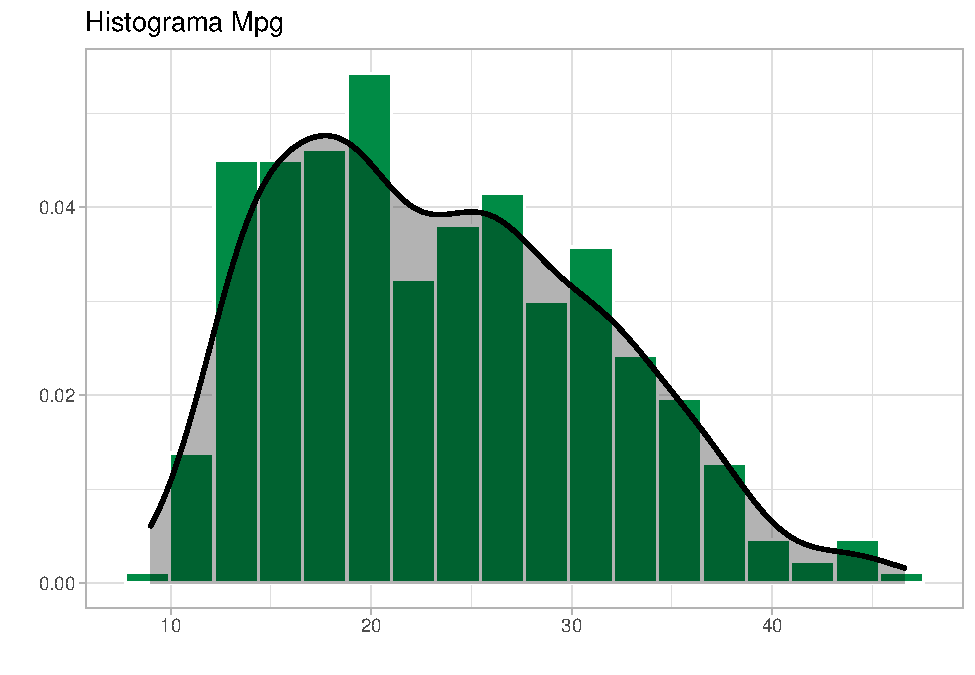
\includegraphics[width=.9\linewidth]{img/EDA_files/figure-latex/unnamed-chunk-7-6} \caption{}\end{figure}

\begin{figure}[H]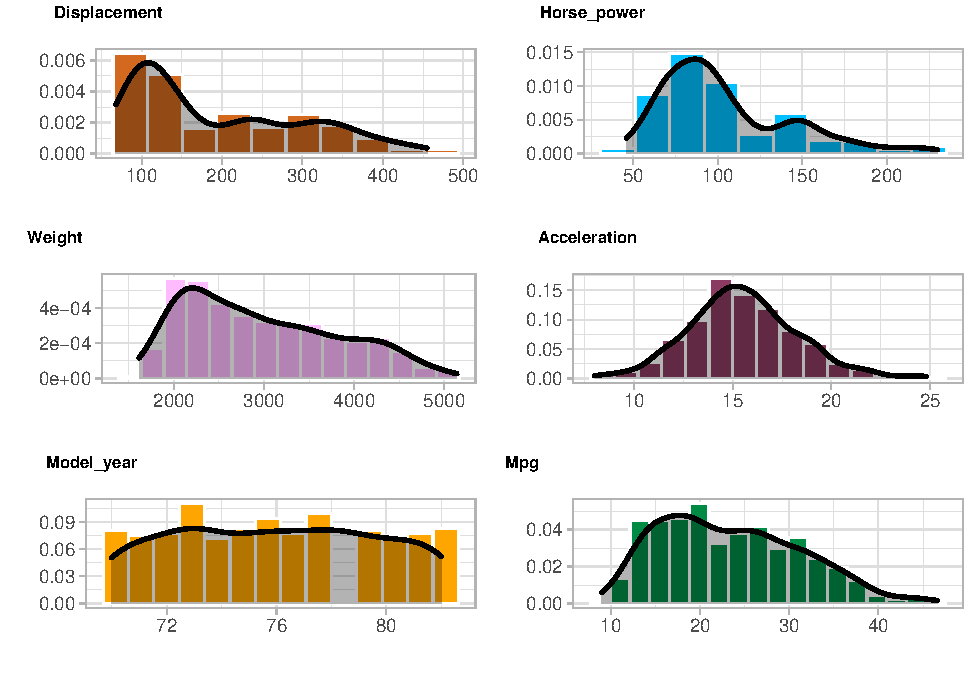
\includegraphics[width=.9\linewidth]{img/EDA_files/figure-latex/unnamed-chunk-7-7} \caption{}\end{figure}

\newpage

Y boxplots sobre las distribuciones de los datos:
\begin{figure}[H]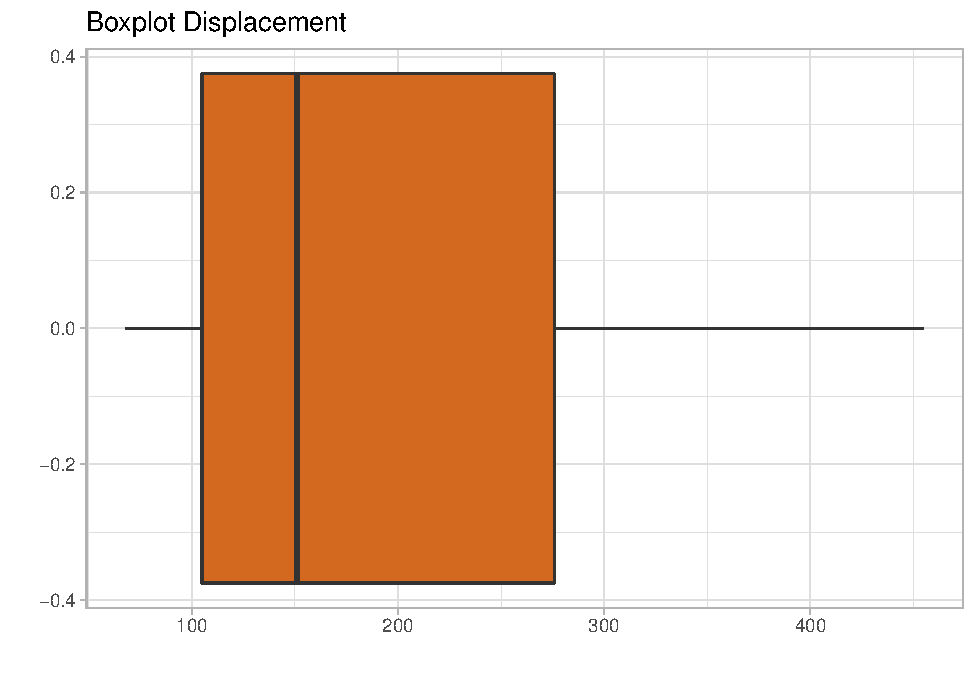
\includegraphics[width=.9\linewidth]{img/EDA_files/figure-latex/unnamed-chunk-8-1} \caption{}\end{figure}
\begin{figure}[H]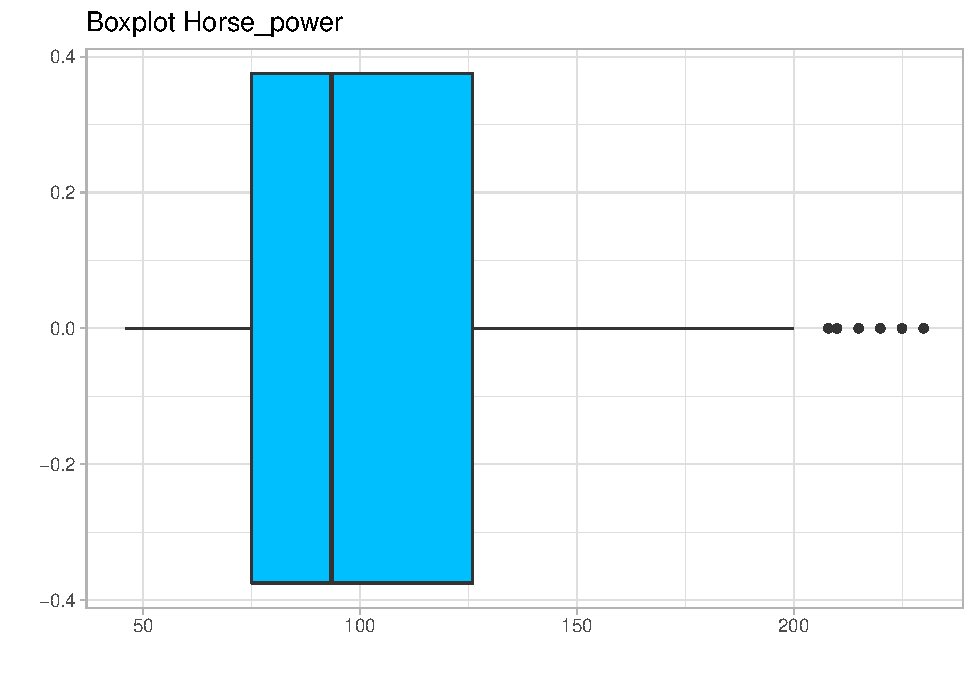
\includegraphics[width=.9\linewidth]{img/EDA_files/figure-latex/unnamed-chunk-8-2} \caption{}\end{figure}
\begin{figure}[H]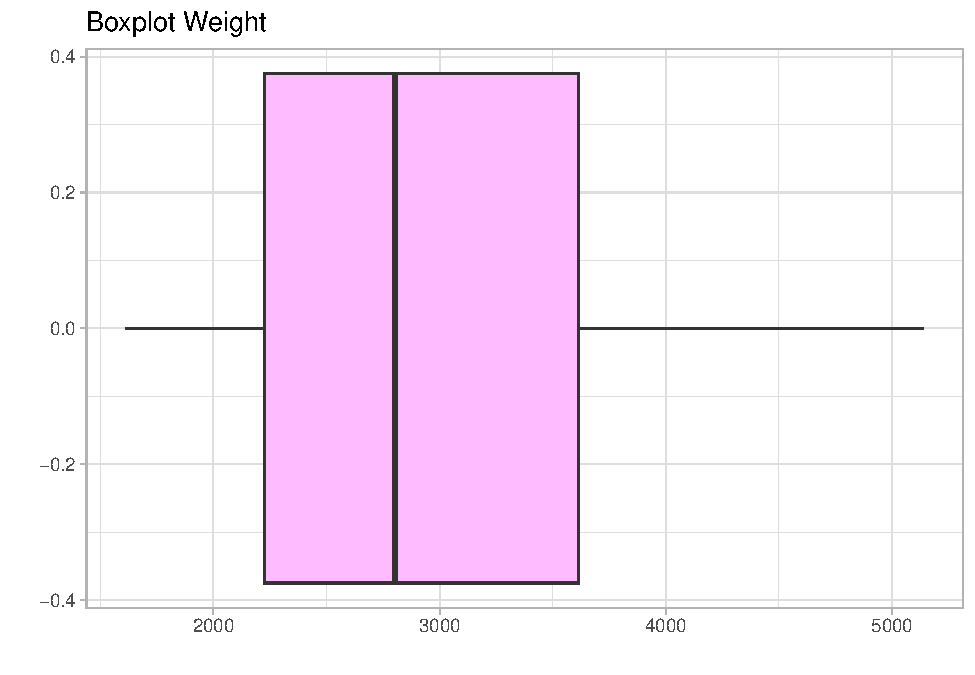
\includegraphics[width=.9\linewidth]{img/EDA_files/figure-latex/unnamed-chunk-8-3} \caption{}\end{figure}
\begin{figure}[H]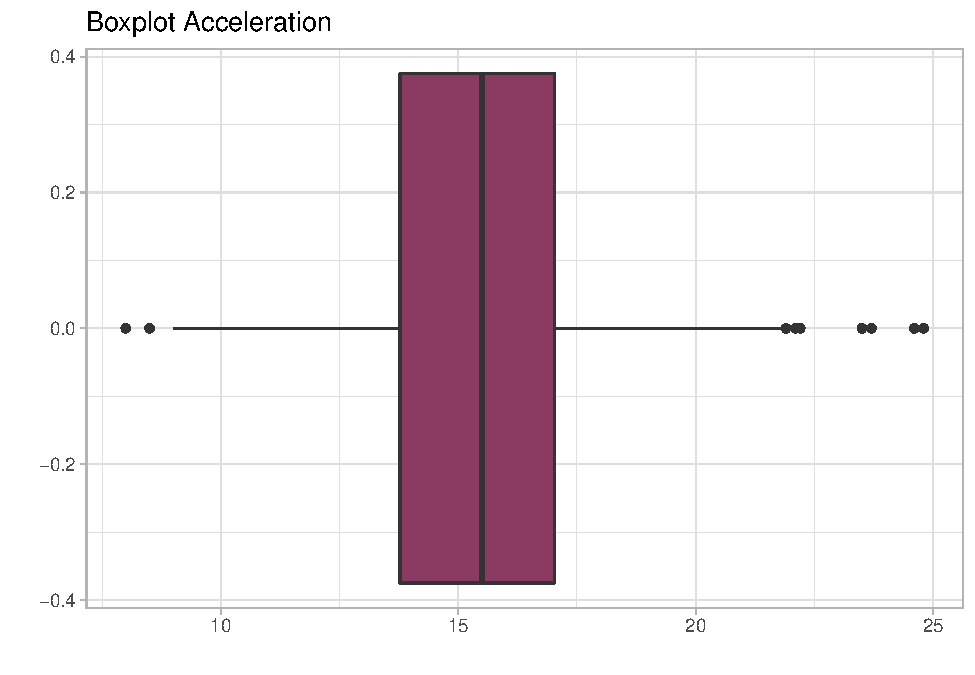
\includegraphics[width=.9\linewidth]{img/EDA_files/figure-latex/unnamed-chunk-8-4} \caption{}\end{figure}
\begin{figure}[H]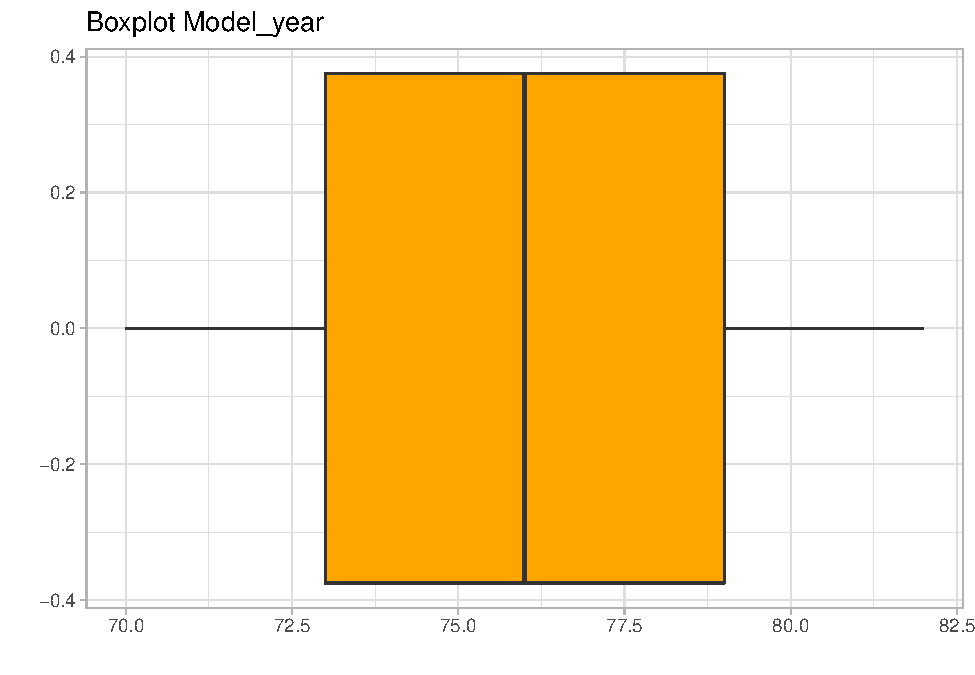
\includegraphics[width=.9\linewidth]{img/EDA_files/figure-latex/unnamed-chunk-8-5} \caption{}\end{figure}
\begin{figure}[H]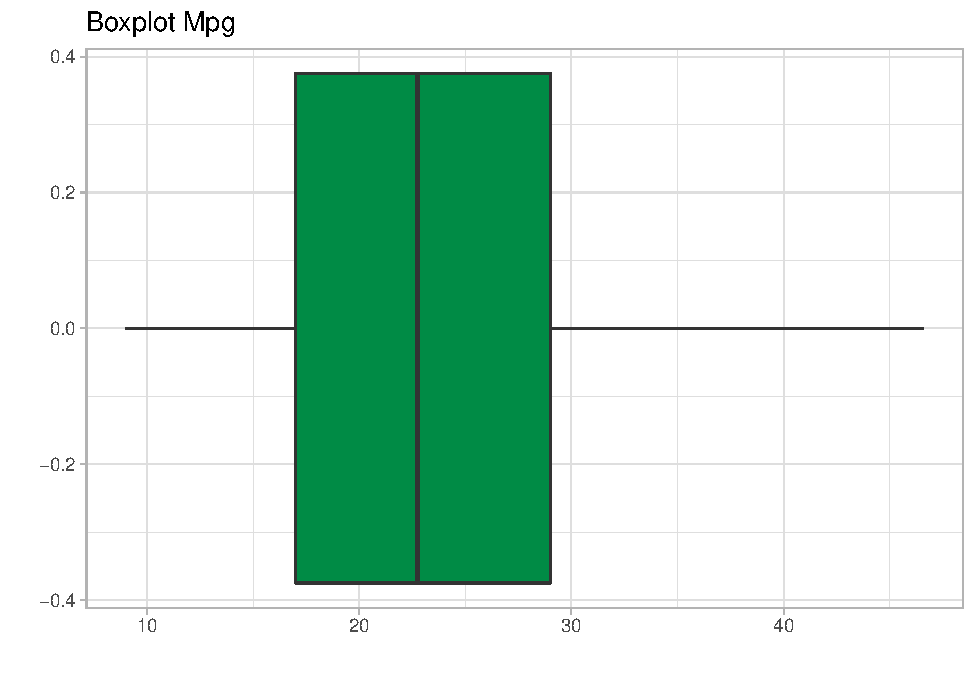
\includegraphics[width=.9\linewidth]{img/EDA_files/figure-latex/unnamed-chunk-8-6} \caption{}\end{figure}

\begin{figure}[H]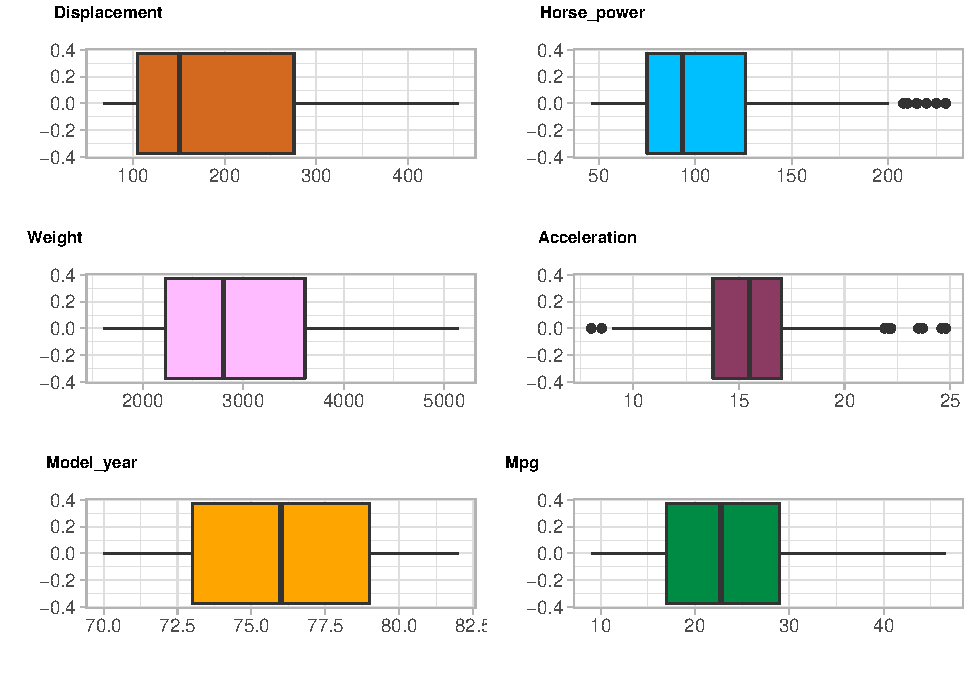
\includegraphics[width=.9\linewidth]{img/EDA_files/figure-latex/unnamed-chunk-8-7} \caption{}\end{figure}
\begin{figure}[H]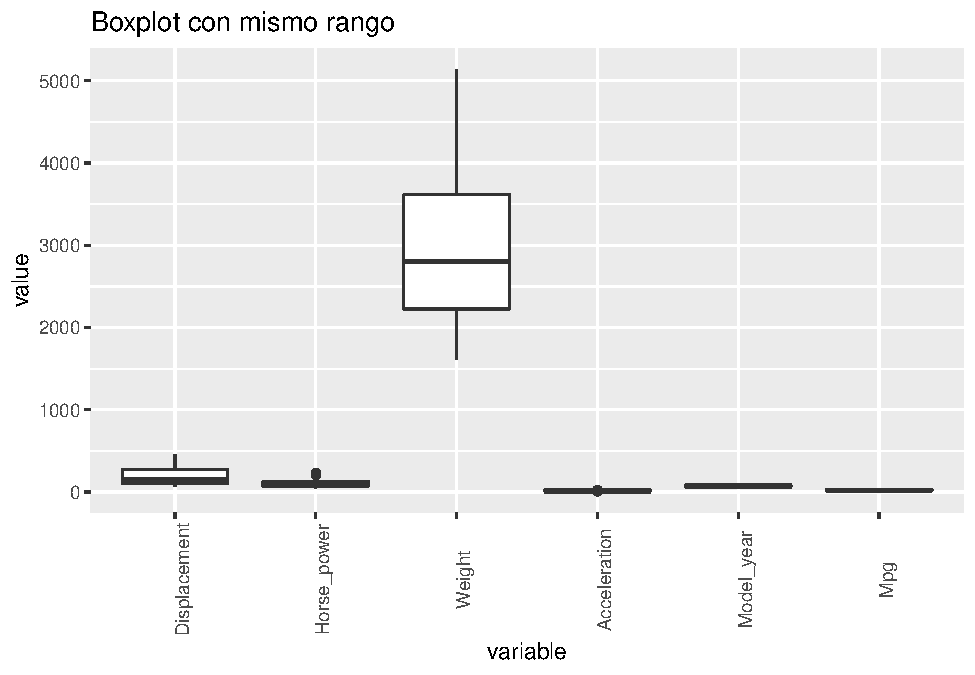
\includegraphics[width=.9\linewidth]{img/EDA_files/figure-latex/unnamed-chunk-9-1} \caption{}\end{figure}
\begin{figure}[H]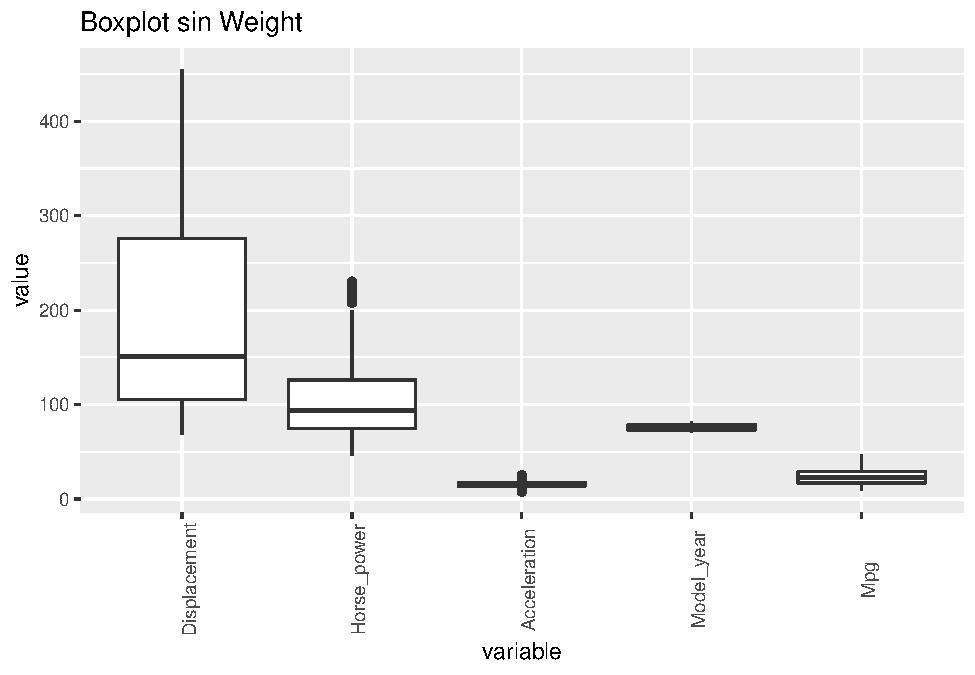
\includegraphics[width=.9\linewidth]{img/EDA_files/figure-latex/unnamed-chunk-9-2} \caption{}\end{figure}

Ya la descripción del problema nos lo decía, los rangos en los que se distribuyen los datos son muy diferentes dependiendo de la variable. Se pueden estandarizar los datos para solucionar este problema, aunque para regresión lineal no es necesario (sí lo es para KNN)
\vspace{\baselineskip}
Podemos comparar los rangos intercuartiles si estandarizamos antes el dataset

\begin{verbatim}
Displacement  Horse_power       Weight Acceleration   Model_year          Mpg 
    1.631723     1.324980     1.635856     1.178021     1.628781     1.537475 
\end{verbatim}

También podemos ver la distancia entre mínimos y máximos

\begin{verbatim}
Displacement  Horse_power       Weight Acceleration   Model_year          Mpg 
    3.698253     4.780318     4.152330     6.089463     3.257562     4.817420 
\end{verbatim}

\paragraph{Displacement}
La cilindrada vemos que cuenta con una desviación grande y una gran concentración en los valores inferiores. Desviado a la izquierda, no parece seguir una distribución normal. Existe una alta concentración en torno al valor 125, muy por encima del recuento que alcanzan el resto de valores.

\paragraph{Horse\_power}
Similar a Displacement pero tiene mayor dispersión y algunos valores muy altos. A día de hoy los coches suelen rondar los 120 en turismos y los 200 en SUVs. Aquí contamos con predominancia en el rango aproximado {[}70, 125{]} con algunas instancias por encima de los 200.
Desviado a la izquierda, tampoco parece seguir una distribución normal.

\paragraph{Weight}
Una distribución más achatada que las anteriores, también ladeada hacia la izquierda. Cuenta con un rango mayor.

\paragraph{Acceleration}
Valores altamente concentrados pero en general con un rango grande. Su forma se asemeja a una distribución normal.

\paragraph{Model\_year}
Aunque no se vea bien en las gráficas, contamos con valores de todos los años, más o menos equitativamente:

\begin{verbatim}
Años:   70 71 72 73 74 75 76 77 78 79 80 81 82 
Conteo: 29 27 28 40 26 30 34 28 36 29 27 28 30 
\end{verbatim}


\subsubsection{Análisis sobre las distribuciones}

Hemos comentado antes que no apreciamos semejanzas con una distribución normal en algunas de las variables, lo comprobamos con un test estadístico (Shapiro-Wilk test):
\vspace{\baselineskip}

\begin{tabular}{l|r|r|r}
\hline
vars & statistic & p\_value & sample\\
\hline
Displacement & 0.8818359 & 0.0000000 & 392\\
\hline
Horse\_power & 0.9040975 & 0.0000000 & 392\\
\hline
Weight & 0.9414661 & 0.0000000 & 392\\
\hline
Acceleration & 0.9918671 & 0.0305289 & 392\\
\hline
Model\_year & 0.9469666 & 0.0000000 & 392\\
\hline
Mpg & 0.9671696 & 0.0000001 & 392\\
\hline
\end{tabular}

\vspace{\baselineskip}

El test de Shapiro nos asegura con bastante certeza que ninguna variable sigue una distribución normal, aunque en menor grado en Acceleration (sigue siendo al 97\% de confianza).

Para los modelos de regresión que vamos a usar aún así la normalidad de los datos no es necesaria.
\vspace{\baselineskip}

Se muestra aquí como no hay que dejarse engañar por los gráficos, puesto que Acceleration parecía seguirla. El p-value de Acceleration está muy cerca del umbral (0.03 vs 0.05). Es bastante probable de que la parte central derecha de la distribución sea la causante de no asegurar la normalidad.

\vspace{\baselineskip}
Mostramos con gráficos Q-Q cómo se separan las distribuciones de su supuesta normal:

\begin{figure}[H]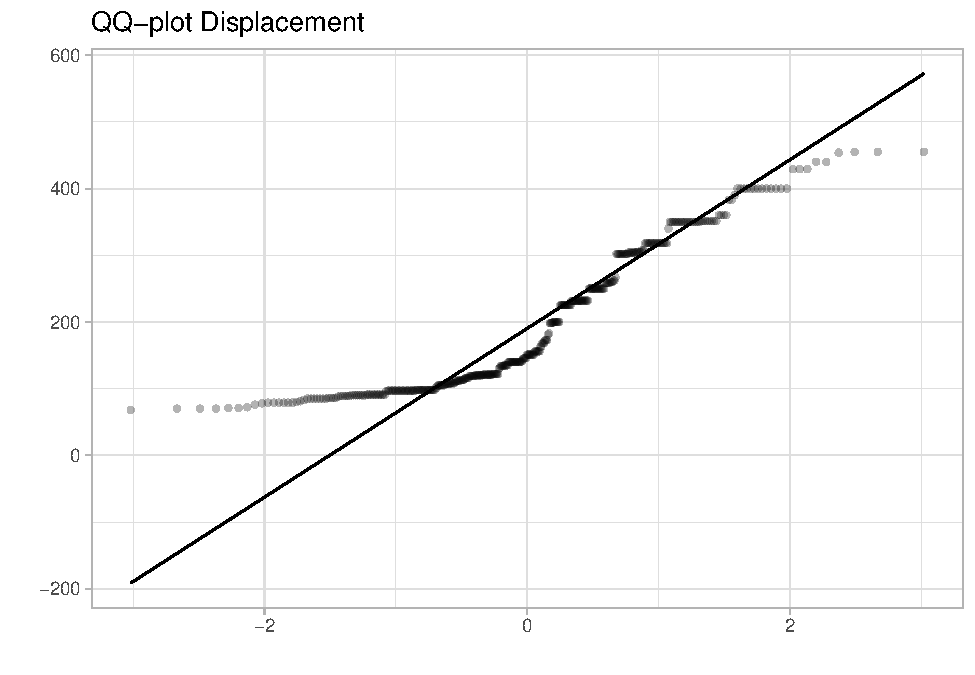
\includegraphics[width=.9\linewidth]{img/EDA_files/figure-latex/unnamed-chunk-14-1} \caption{}\end{figure}

\begin{figure}[H]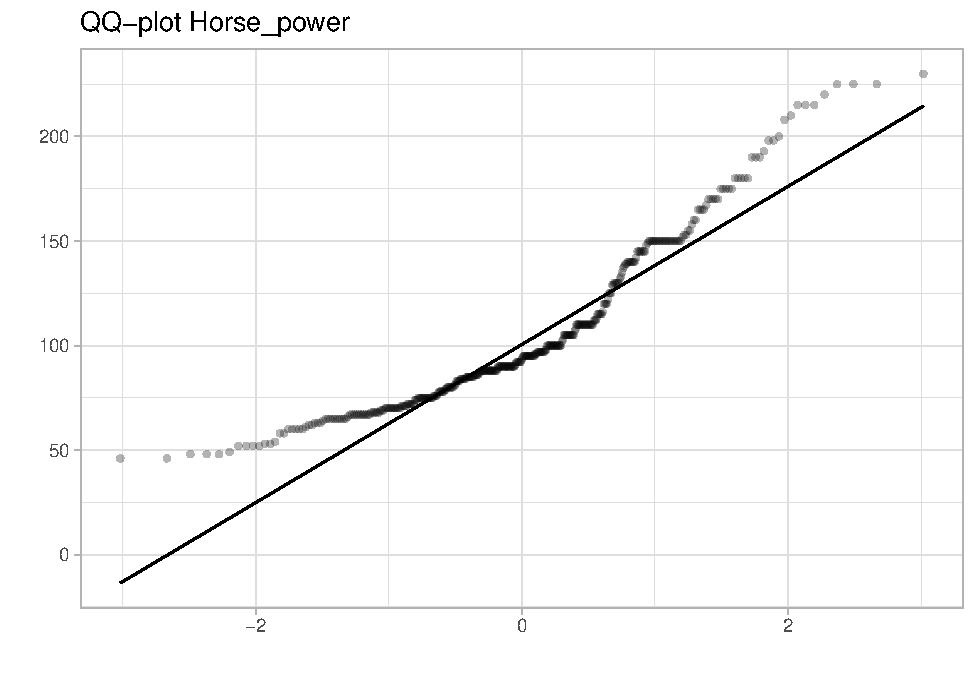
\includegraphics[width=.9\linewidth]{img/EDA_files/figure-latex/unnamed-chunk-14-2} \caption{}\end{figure}

\begin{figure}[H]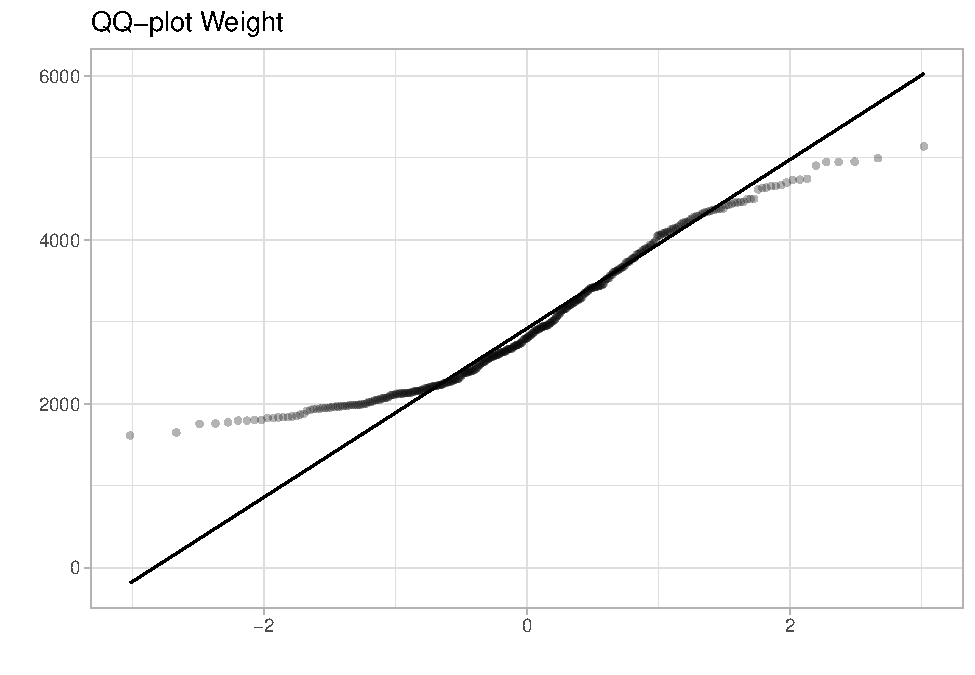
\includegraphics[width=.9\linewidth]{img/EDA_files/figure-latex/unnamed-chunk-14-3} \caption{}\end{figure}

\begin{figure}[H]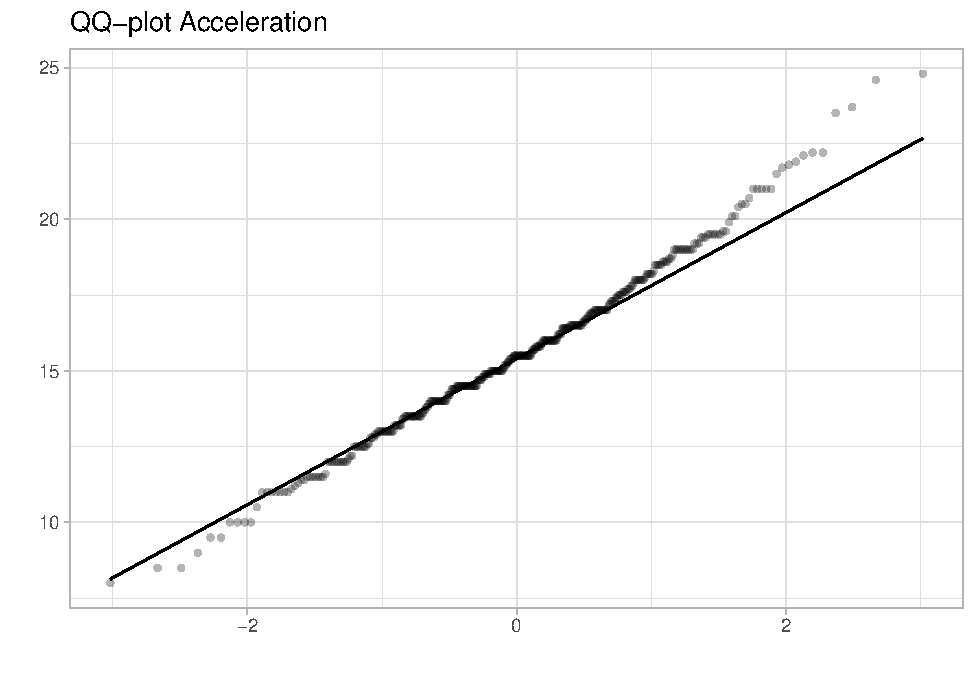
\includegraphics[width=.9\linewidth]{img/EDA_files/figure-latex/unnamed-chunk-14-4} \caption{}\end{figure}

\begin{figure}[H]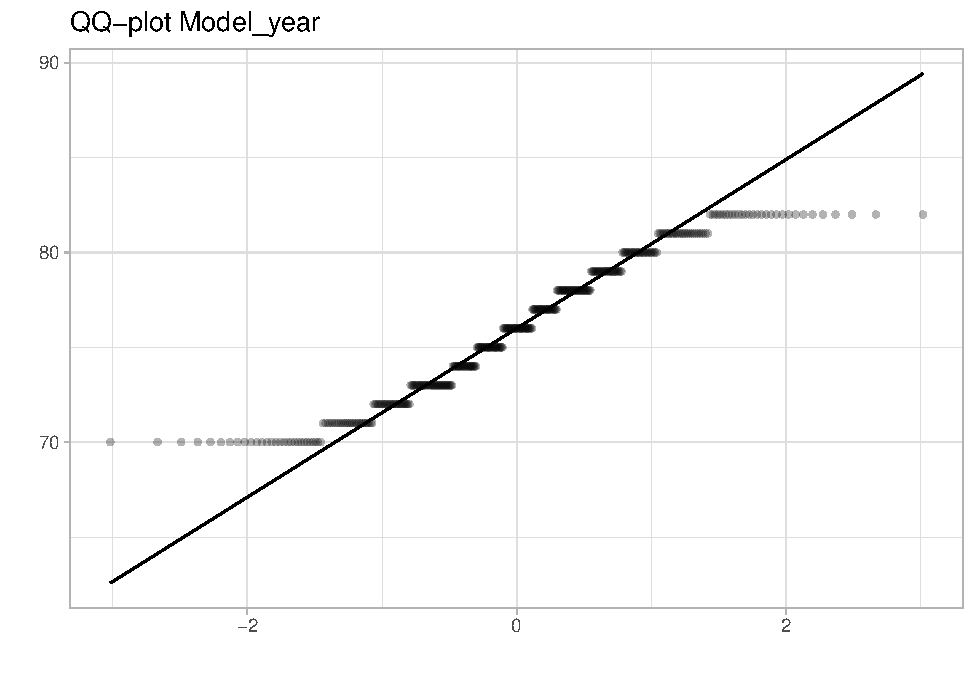
\includegraphics[width=.9\linewidth]{img/EDA_files/figure-latex/unnamed-chunk-14-5} \caption{}\end{figure}

\begin{figure}[H]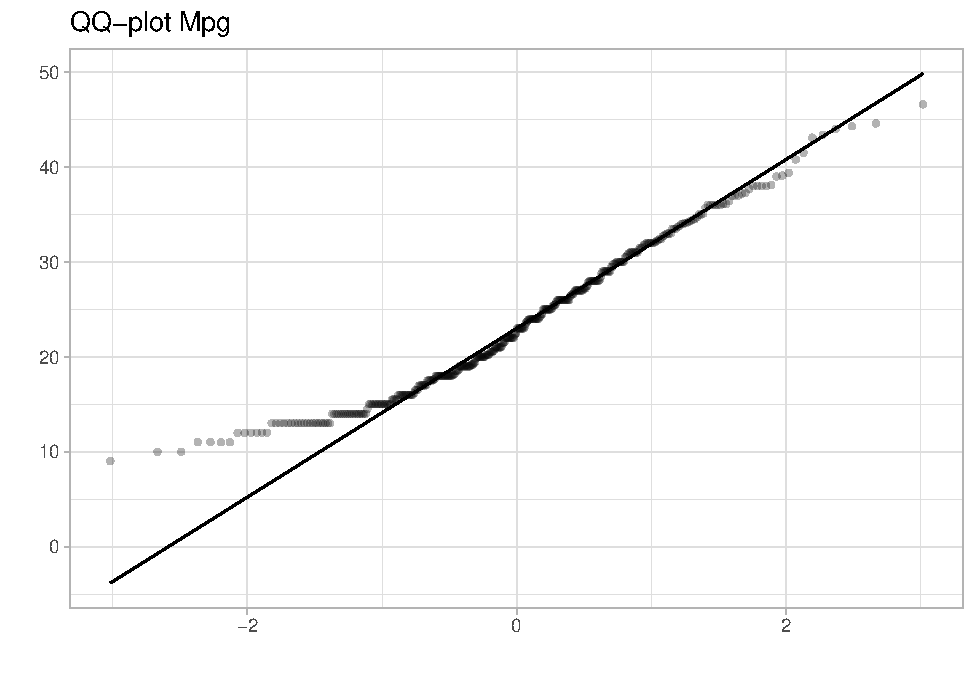
\includegraphics[width=.9\linewidth]{img/EDA_files/figure-latex/unnamed-chunk-14-6} \caption{}\end{figure}

\begin{figure}[H]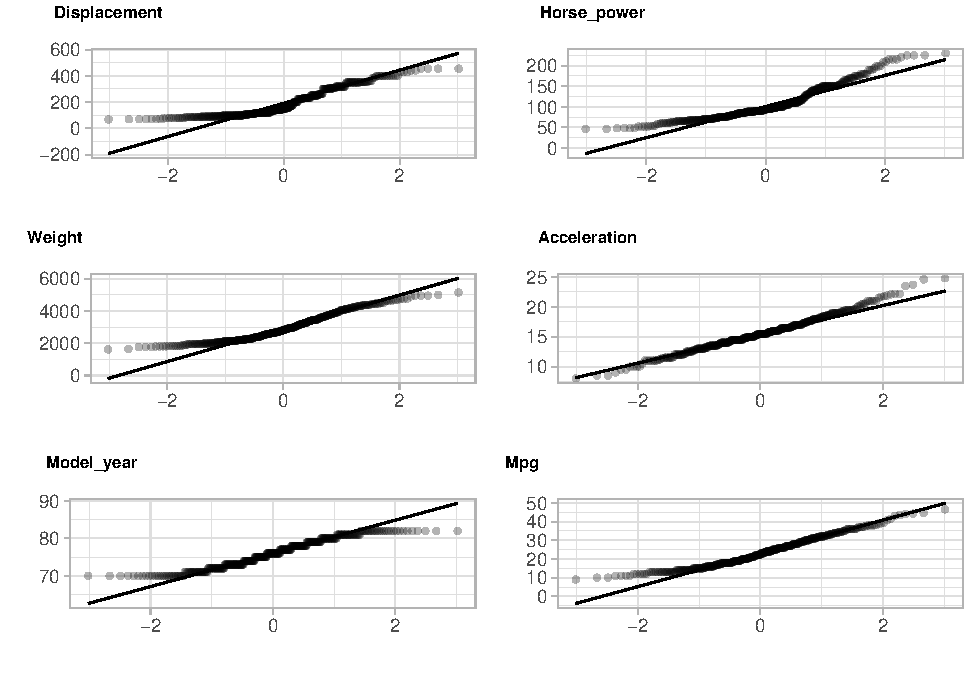
\includegraphics[width=.9\linewidth]{img/EDA_files/figure-latex/unnamed-chunk-14-7} \caption{}\end{figure}

Estos gráficos Q-Q nos muestran más claramente que las variables no siguen distribuciones normales. La distribución de Acceleration es la que más se asemeja y eso lo vemos en el estadístico de Shapiro, pero en la cola superior existe una diferencia significativa que hace que el test rechace.

\paragraph{Skewness}
Contamos con 3 variables de skewness, todas positivas (hacia la izquierda):

\begin{verbatim}
Displacement:  0.6989813
Horse_power:  1.083161
Weight:  0.5175953

Adicionalmente, se muestra:
Mpg:  0.4553414
\end{verbatim}

Los plots nos han dado idea de que Mpg tiene cierta skewness, pero cae por debajo del umbral de 0.5.

\subsubsection{Transformaciones}
En general no consideramos que sea necesaria ninguna transformación para el dataset con el que contamos.
Tampoco vemos necesario crear variables nuevas a partir de las vistas, puesto que por el conocimiento que tenemos del problema parece que las variables son coherentes.

Las transformaciones necesarias para pasar a una distribución normal dependen de la variable en cuestión. Primero deberíamos averiguar que tipo de distribución siguen.
Pese a ello, tal y como se ha comentado anteriormente, los métodos utilizados para regresión (regresión lineal y KNN) no asumen ninguna forma para la distribución de los datos, por lo que no es necesario aplicar nada.

Adicionalmente, aunque para regresión lineal tampoco es absolutamente necesario, podemos estandarizar los datos a media 0 y desviación típica 1, facilitando un poco los cálculos. La inferencia estadística de la regresión no variaría, pero deberíamos tener cuidado a la hora de interpretar los resultados para no confundirnos.

\subsubsection{Outliers}
Como hemos visto anteriormente en los boxplots, las únicas variables con valores muy alejados del centro de la distribución son Acceleration y Horse\_power.

\vspace{\baselineskip}

Por el significado del problema, probablemente estos posibles outliers correspondan a coches de alta gama o potentes en la época. Esto tampoco lo podemos asegurar puesto que no contamos con las características suficientes, pero se considera un razonamiento coherente. Además, puesto que los valores caen dentro de los rangos posibles para coches de la época, podemos descartar que sean errores de medida.

Deberíamos decidir si mantener o no estas instancias. Como en nuestro caso se nos ha pedido predecir el consumo Mpg, sin darnos consideraciones sobre los tipos/gamas de coches a los que se enfoca, proseguimos dejándo estas filas.

\subsubsection{Análisis de correlación}

Tenemos que tener en cuenta que las variables no siguen distribuciones normales. Aunque el coeficiente de Pearson no asume normalidad (si asume varianza y covarianza finitas), podemos adicionalmente usar el coeficiente de Kendall. Independientemente del método usado vamos a obtener las mismas correlaciones en este dataset, solo varía el valor de fuerza con la que se dan.

\vspace{\baselineskip}

Para regresión la correlación en los datos no es preocupante. Al contrario, podría haber información (poca, pero alguna cantidad) que se aporte y nos ayude en el problema. En el peor de los casos, la propia metodología de selección de variables en el modelo multivariable nos ayudará a descartar aquellas variables que no sean necesarias como regresor.

\begin{figure}[H]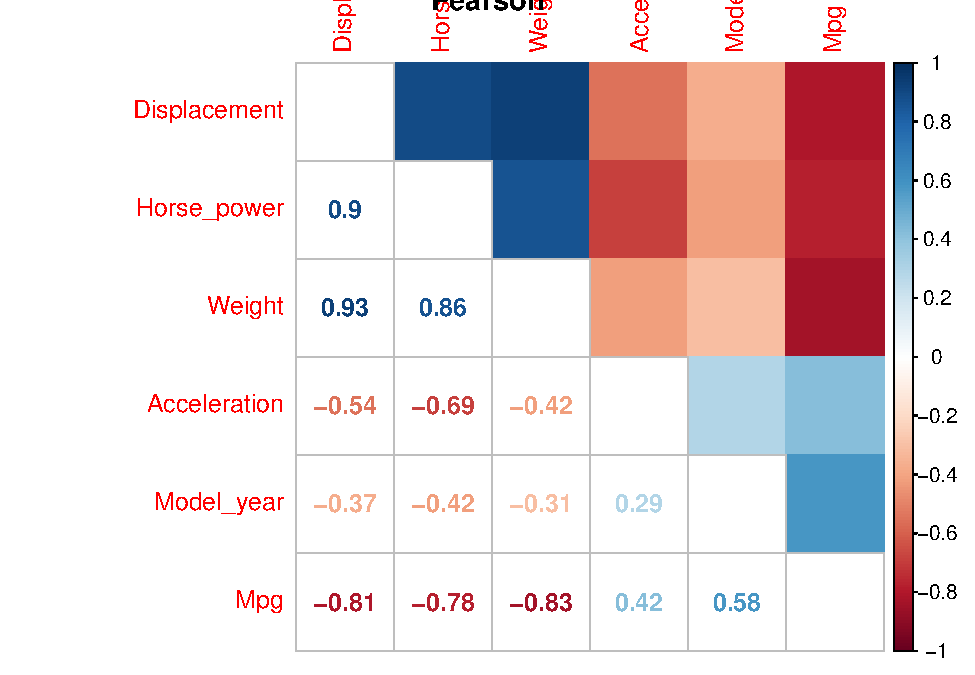
\includegraphics[width=.9\linewidth]{img/EDA_files/figure-latex/unnamed-chunk-19-1} \caption{}\end{figure}
\begin{figure}[H]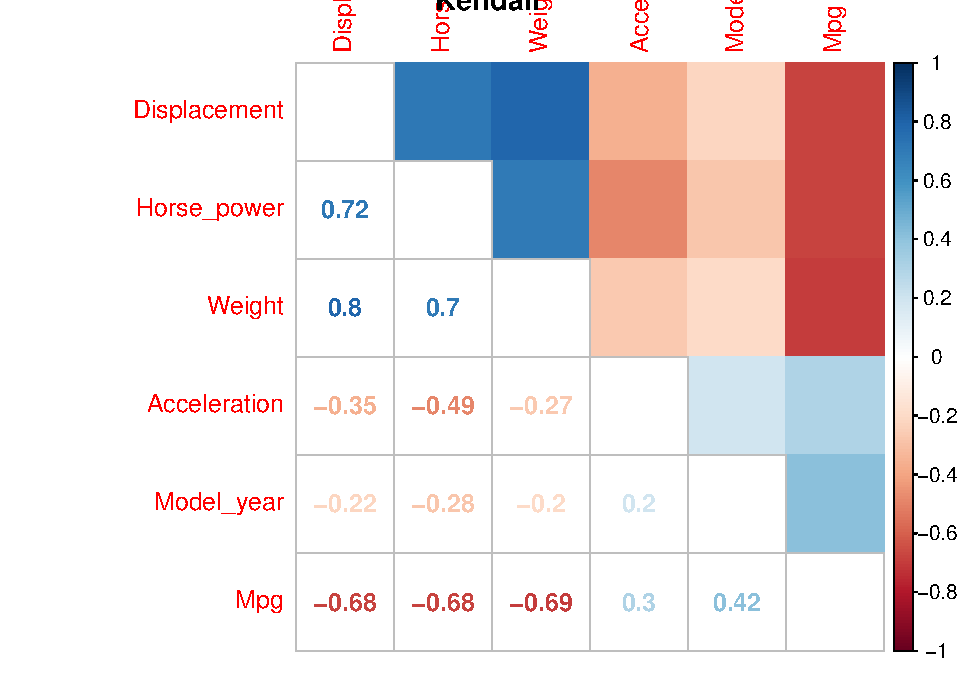
\includegraphics[width=.9\linewidth]{img/EDA_files/figure-latex/unnamed-chunk-19-2} \caption{}\end{figure}

\newpage

Estas gráficas nos dicen que existe una alta correlación en el dataset, generalmente entre todas las variables (a excepción de Model\_year), pero extremadamente fuerte en las parejas:

\begin{enumerate}
    \def\labelenumi{\arabic{enumi}.}
    \item   Horse\_power \& Displacement
    \item   Weight \& Displacement
    \item   Weight \& Horse\_power
    \item   Acceleration \& Horse\_power
    \item   Mpg \& Horse\_power
    \item   Mpg \& Displacement
    \item   Mpg \& Weight
\end{enumerate}

\begin{figure}[H]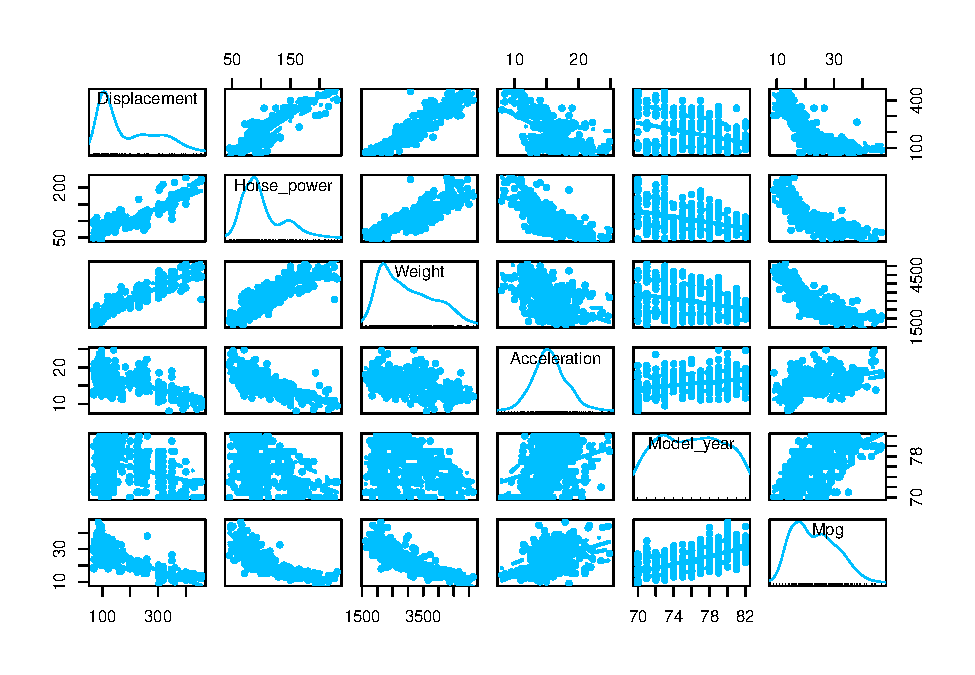
\includegraphics[width=.9\linewidth]{img/EDA_files/figure-latex/unnamed-chunk-20-1} \caption{}\end{figure}

El scatterplot anterior nos muestra mejor la forma de estas correlaciones. Vemos que en todos los casos en los que se da una correlación positiva existe una tendencia lineal entre los datos de ambas variables, y en las negativas una tendencia logarítmica.

% \vspace{\baselineskip}
\newpage

Vamos a mostrar algunas parejas con correlación positiva:

\begin{figure}[H]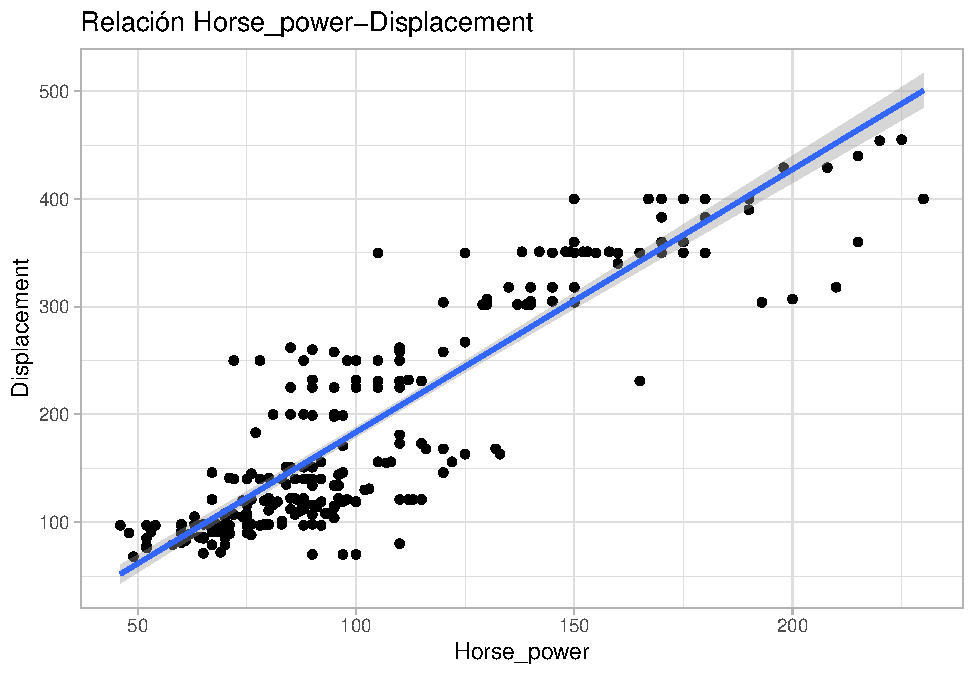
\includegraphics[width=.9\linewidth]{img/EDA_files/figure-latex/unnamed-chunk-21-1} \caption{}\end{figure}
\begin{figure}[H]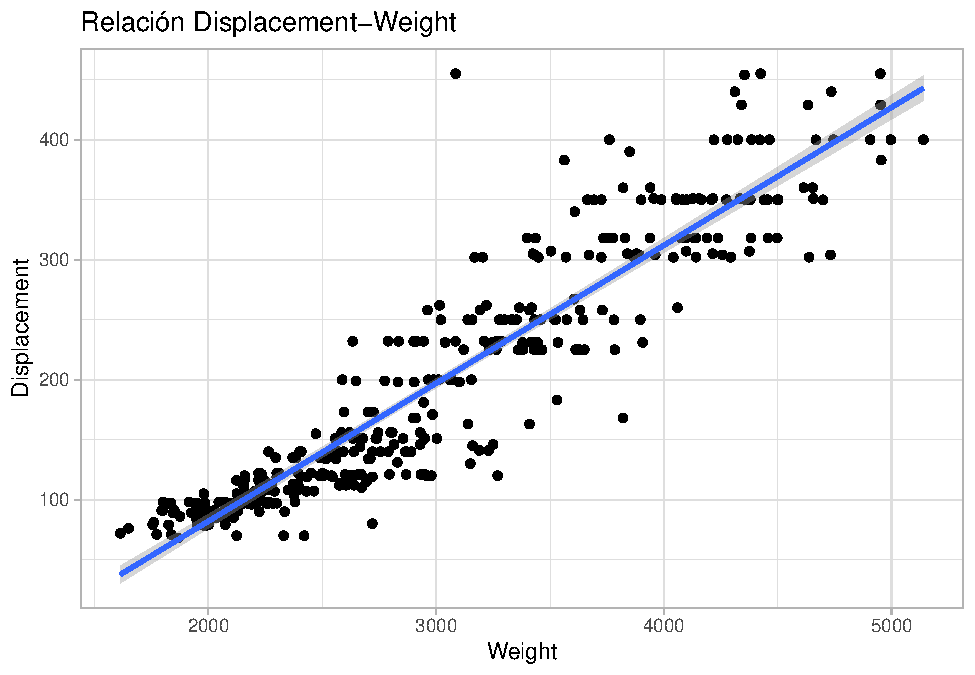
\includegraphics[width=.9\linewidth]{img/EDA_files/figure-latex/unnamed-chunk-21-2} \caption{}\end{figure}

Y otras con correlación negativa:

\begin{figure}[H]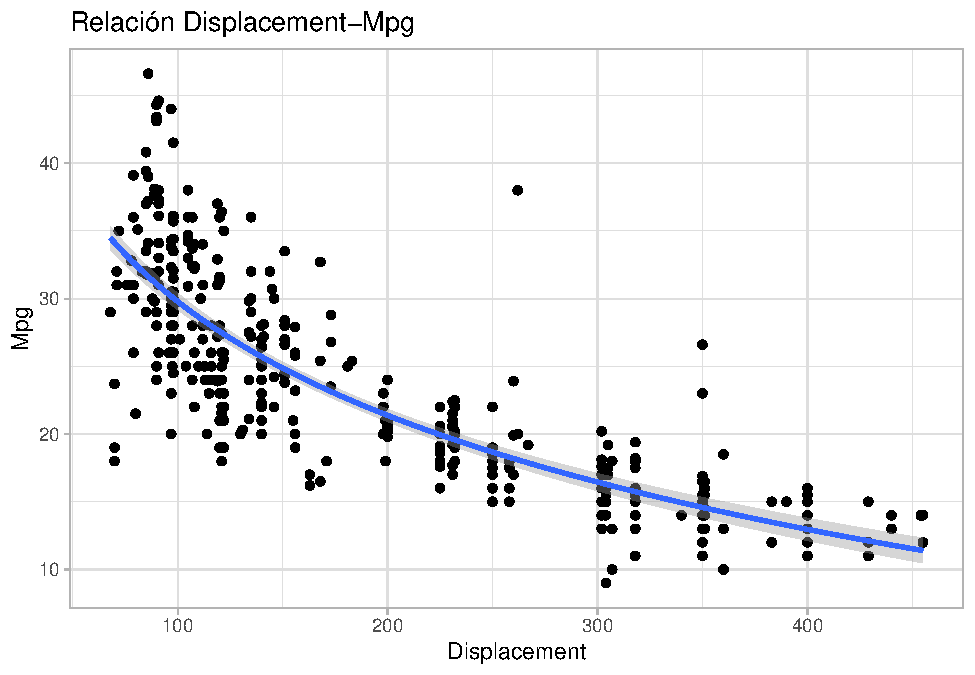
\includegraphics[width=.9\linewidth]{img/EDA_files/figure-latex/unnamed-chunk-22-1} \caption{}\end{figure}
\begin{figure}[H]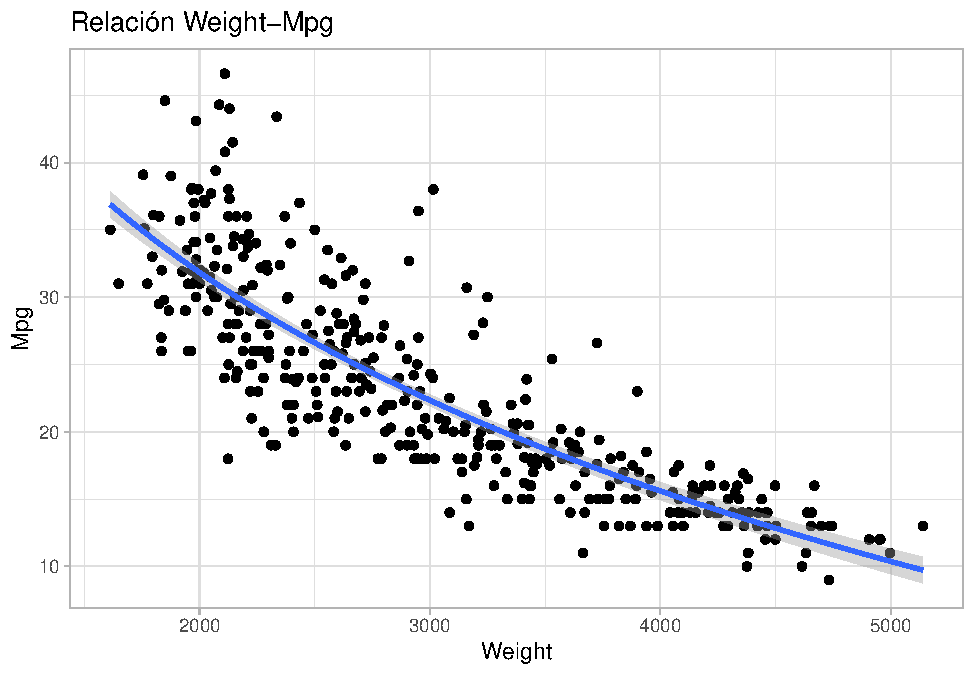
\includegraphics[width=.9\linewidth]{img/EDA_files/figure-latex/unnamed-chunk-22-2} \caption{}\end{figure}

También podemos visualizar los regresores respecto a la salida:

\begin{figure}[H]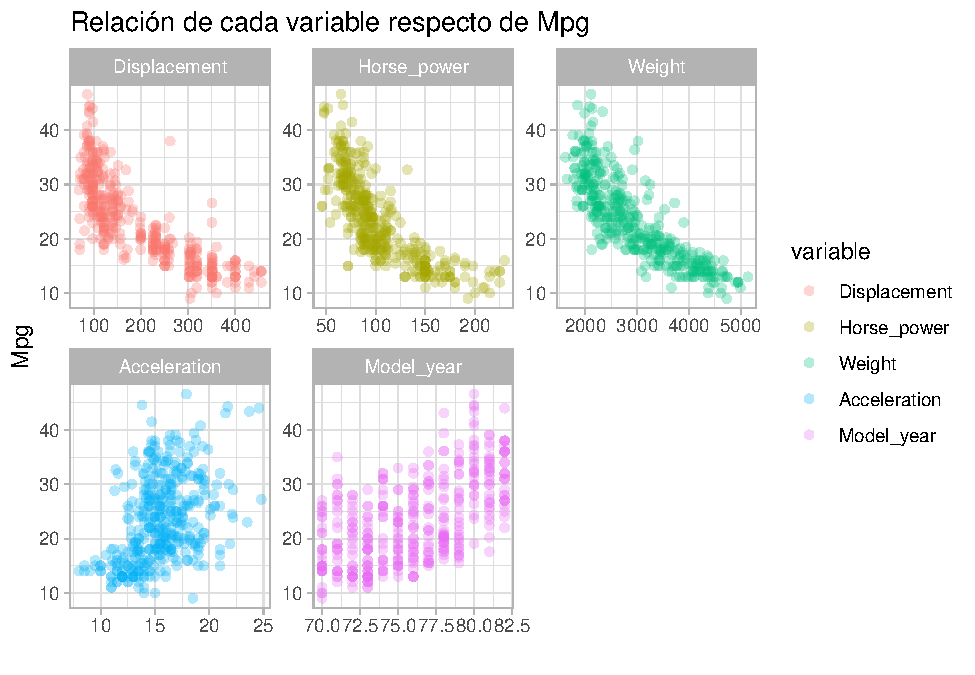
\includegraphics[width=.9\linewidth]{img/EDA_files/figure-latex/unnamed-chunk-23-1} \caption{}\end{figure}

Como habíamos visto, existe alta correlación entre Displacement, Horse\_power, Weight respecto de Mpg.

\vspace{\baselineskip}

Haciendo referencia a la hipótesis H.9, Horse\_power podría depender de Displacement y Weight. Parece bastante probable que la potencia de un motor dependa de la cilindrada y el peso que tenga.

\begin{figure}[H]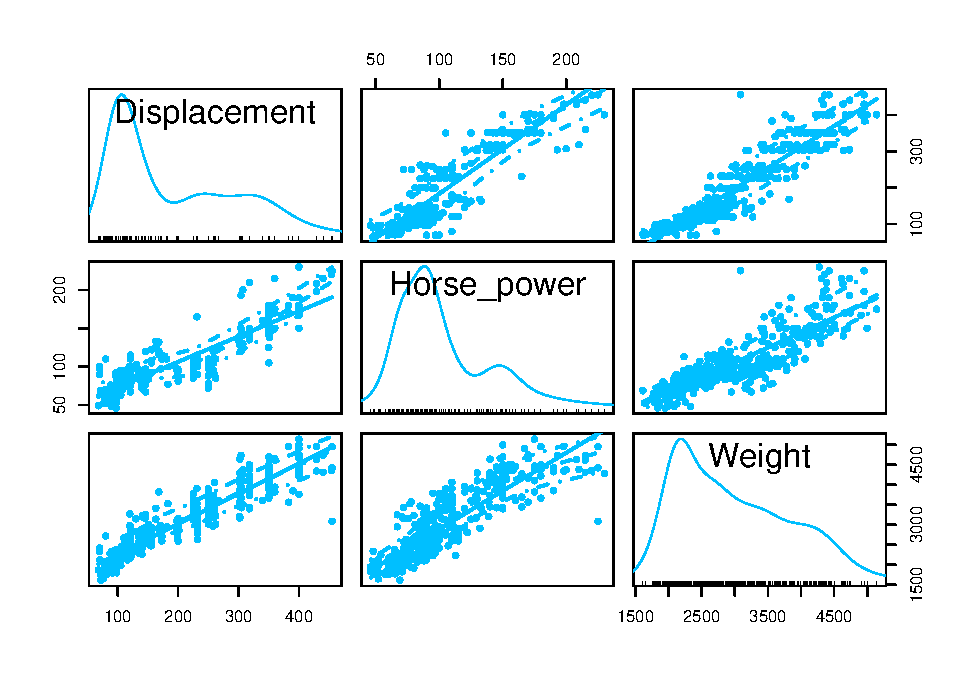
\includegraphics[width=.9\linewidth]{img/EDA_files/figure-latex/unnamed-chunk-24-1} \caption{}\end{figure}

Viendo las funciones de densidad, buscamos ver si la media de las dos variables se asemeja con la distribución de Horse\_power.

\begin{figure}[H]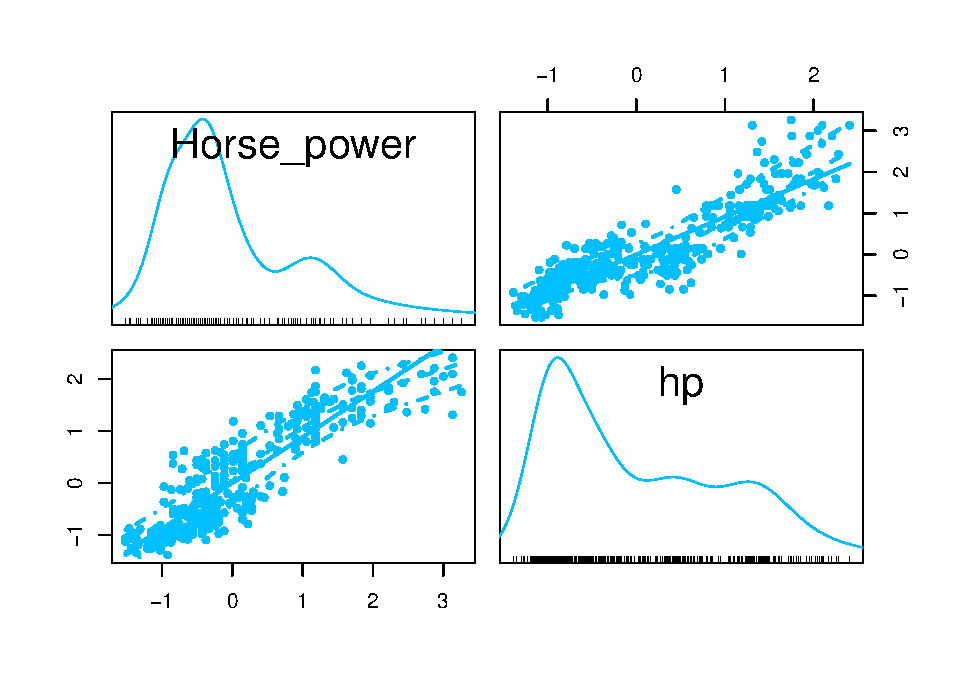
\includegraphics[width=.9\linewidth]{img/EDA_files/figure-latex/unnamed-chunk-25-1} \caption{}\end{figure}

Viendo que no son tan similares como creíamos, buscamos diferentes fórmulas \cite{horsepower} para el cálculo de los caballos de vapor. Las fórmulas son un poco más complejas y no tenemos exactamente los datos necesarios para utilizarlas (no se descarta que no se puedan deducir, pero no sería un cálculo evidente).

\subsubsection{Tratamiento de variables}

Para este dataset, al ser casi todas las variables numéricas continuas, existen pocos tratamientos que aplicar.

Para añadir interpretabilidad, podríamos agrupar la variable Weight en intervalos, pero puesto que vamos a aplicar regresión sería más conveniente realizarlo con los resultados finales.

\subsubsection{Ordenaciones}

Volvemos a mostrar la cabecera de los datos:
\vspace{\baselineskip}

\begin{tabular}{r|r|r|r|r|r}
\hline
Displacement & Horse\_power & Weight & Acceleration & Model\_year & Mpg\\
\hline
91 & 70 & 1955 & 20.5 & 71 & 26.0\\
\hline
232 & 100 & 2789 & 15.0 & 73 & 18.0\\
\hline
350 & 145 & 4055 & 12.0 & 76 & 13.0\\
\hline
318 & 140 & 4080 & 13.7 & 78 & 17.5\\
\hline
113 & 95 & 2372 & 15.0 & 70 & 24.0\\
\hline
97 & 60 & 1834 & 19.0 & 71 & 27.0\\
\hline
\end{tabular}

\vspace{\baselineskip}

En este caso no es necesario aplicar ninguna reorganización. Cada variable ocupa su propia columna y contiene un único tipo de información, con unidades de observación diferentes. Tampoco existe ninguna relación entre variables sobre la información que codifican (en el sentido de que podrían agruparse).

\subsubsection{Resolución de hipótesis}

Nos habíamos planteado las siguientes hipótesis

\begin{itemize}
\item \textbf{H.1}: Horse\_power puede influir en Mpg: A más potencia, más consumo.
\end{itemize}

\begin{figure}[H]\center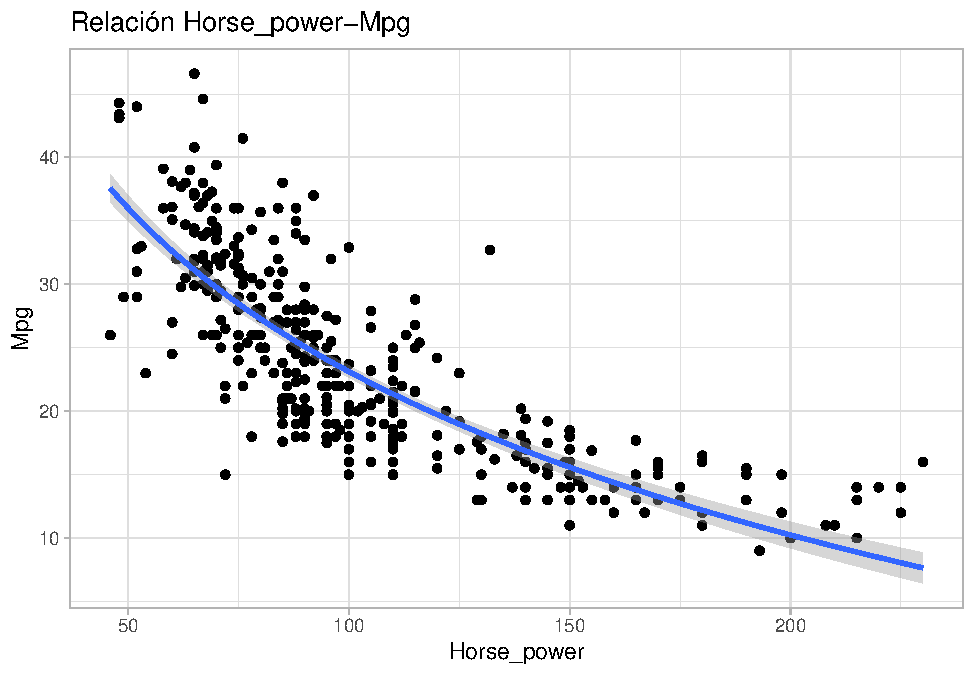
\includegraphics[width=.56\linewidth]{img/EDA_files/figure-latex/unnamed-chunk-27-1} \caption{}\end{figure}

Con el plot y los resultados de la matriz de correlación queda claro que existe una correlación negativa entre estas dos variables. Por tanto, podemos considerar Horse\_power como un buen candidato para la regresión

\begin{itemize}
\item \textbf{H.2}: Weight debe influir en Mpg: Un coche más pesado debería consumir más. 

Misma idea que en la hipótesis anterior, lo hemos visto anteriormente en la figura 30.

\item \textbf{H.3}: Debería haber correlación entre displacement (cilindrada) con horse y acceleration. 

La hemos referenciado anteriormente.

\item \textbf{H.4}: Horse y acceleration podrían estar relacionadas
\end{itemize}

\begin{figure}[H]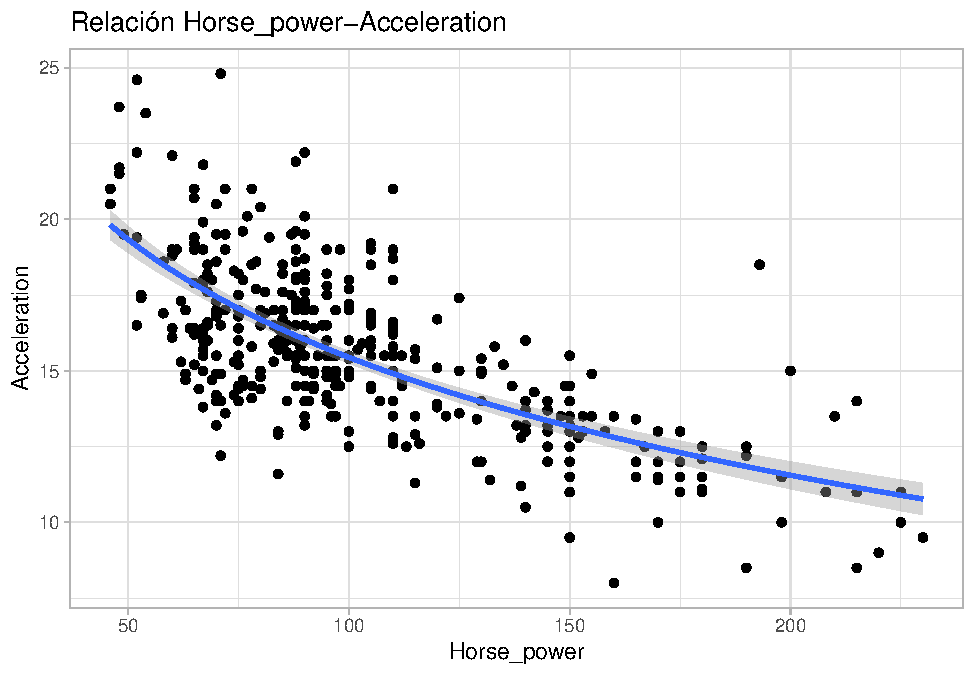
\includegraphics[width=.9\linewidth]{img/EDA_files/figure-latex/unnamed-chunk-28-1} \caption{}\end{figure}

Se aprecia una correlación con forma logarítmica entre las dos variables.

\newpage

\begin{itemize}
\item \textbf{H.5}: Viendo que contamos con un rango pequeño de años, no debería haber un cambio significativo de prestaciones entre años.
\end{itemize}

\begin{figure}[H]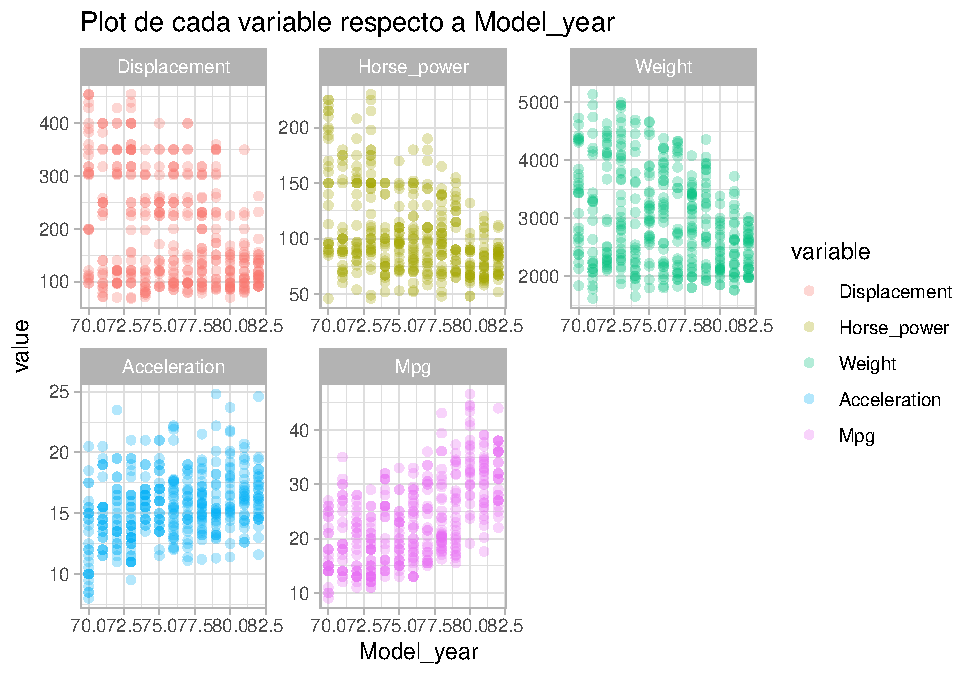
\includegraphics[width=.9\linewidth]{img/EDA_files/figure-latex/unnamed-chunk-29-1} \caption{}\end{figure}

Existe una alta dispersión de los datos en cada una de las variables, pero aún así se aprecia tendencias en las variables. Acceleration y Mpg tienden a aumentar, y Displacement, Horse\_power y Weight tienden a disminuir. También vemos que la dispersión en las prestaciones de los coches disminuyen ligeramente.

\vspace{\baselineskip}

Podríamos creer en principio que puede deberse a un decremento del número de instancias con el paso de los años, pero recordamos que en general los datos están repartidos equitativamente

\begin{verbatim}
Años:   70 71 72 73 74 75 76 77 78 79 80 81 82 
Conteo: 29 27 28 40 26 30 34 28 36 29 27 28 30 
\end{verbatim}

Podemos ver cómo varían los rangos para cada año

\begin{verbatim}
Year  Displacement Horse_power Weight Acceleration Model_year  Mpg
70     97          46          1835    8.0          70          9
       455         225         4732    20.5         70         27
Year  Displacement Horse_power Weight Acceleration Model_year  Mpg
71     71          60          1613    11.5         71         12
       400         180         5140    20.5         71         35
Year  Displacement Horse_power Weight Acceleration Model_year  Mpg
72     70          54          2100    11.0         72         11
       429         208         4633    23.5         72         28
Year  Displacement Horse_power Weight Acceleration Model_year  Mpg
73     68          46          1867    9.5          73         11
       455         230         4997    21.0         73         29
Year  Displacement Horse_power Weight Acceleration Model_year  Mpg
74     71          52          1649    13.5         74         13
       350         150         4699    21.0         74         32
Year  Displacement Horse_power Weight Acceleration Model_year  Mpg
75     90          53          1795    11.5         75         13
       400         170         4668    21.0         75         33
Year  Displacement Horse_power Weight Acceleration Model_year  Mpg
76     85          52          1795    12.0         76         13
       351         180         4380    22.2         76         33
Year  Displacement Horse_power Weight Acceleration Model_year  Mpg
77     79          58          1825    11.1         77         15
       400         190         4335    19.0         77         36
Year  Displacement Horse_power Weight Acceleration Model_year  Mpg
78     78          48          1800    1.2          78         16.2
       318         165         4080    21.5         78         43.1
Year  Displacement Horse_power Weight Acceleration Model_year  Mpg
79     85          65          1915    11.3         79         15.5
       360         155         4360    24.8         79         37.3
Year  Displacement Horse_power Weight Acceleration Model_year  Mpg
80     70          48          1845    11.4         80         19.1
       225         132         3381    23.7         80         46.6
Year  Displacement Horse_power Weight Acceleration Model_year  Mpg
81     79          58          1755    12.6         81         17.6
       350         120         3725    20.7         81         39.1
Year  Displacement Horse_power Weight Acceleration Model_year  Mpg
82     91          52          1965    11.6         82         22
       262         112         3015    24.6         82         44
\end{verbatim}

\begin{itemize}
\item \textbf{H.6}: Pero debería existir una tendencia de mejora de prestaciones con los años, incluyendo aumento de Displacement, Horse\_power y Acceleration.
\end{itemize}

Ciertamente. Se ha comprobado en la hipótesis anterior.

\begin{itemize}
\item \textbf{H.7}: Model\_year podría no mostrar relación con Mpg: Pese al paso de los años si contamos con diferentes tipos de vehículos (todoterrenos, familiares, deportivos\ldots) podría haber un consumo dispar. (Si existiera tendencia, viendo que los años son de las últimas décadas
  del siglo XX, podría ir el consumo hacia abajo)
\end{itemize}

Hemos visto que existe tendencia lineal con gran dispersión, y positiva.

\begin{figure}[H]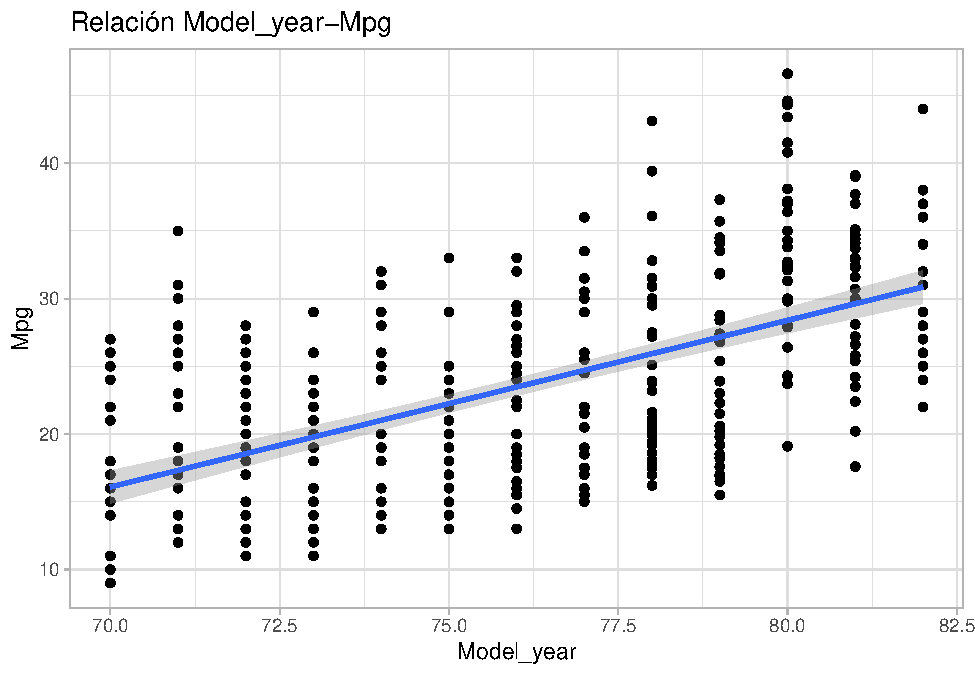
\includegraphics[width=.9\linewidth]{img/EDA_files/figure-latex/unnamed-chunk-32-1} \caption{}\end{figure}

Por desgracia no contamos información sobre los modelos de los coches.

\vspace{\baselineskip}

Podemos ver como se ubican los diferentes años en un plot Horse\_power vs Mpg:

\begin{figure}[H]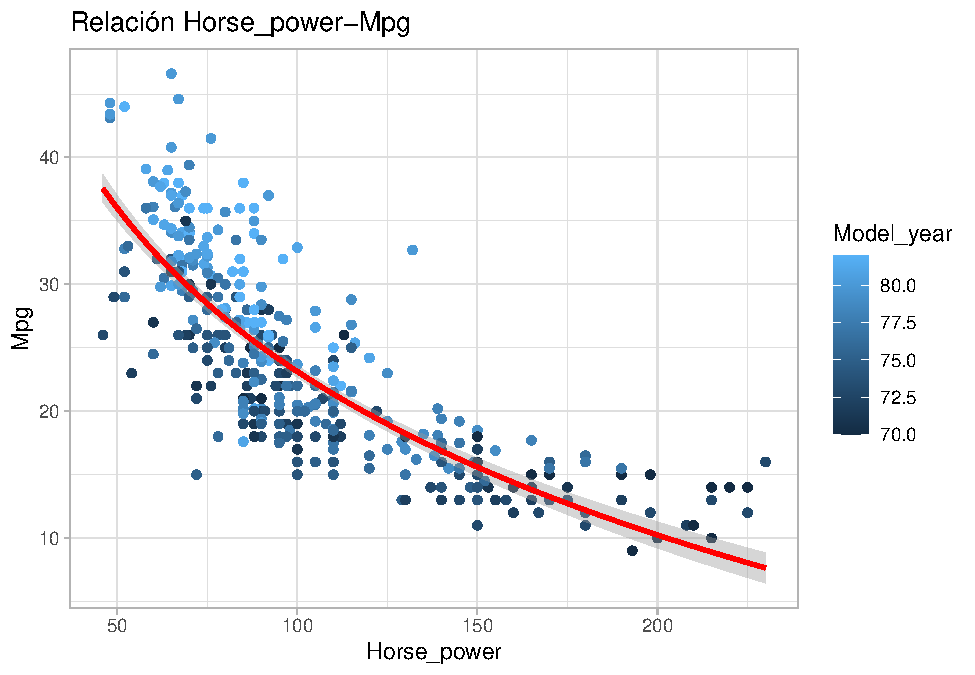
\includegraphics[width=.9\linewidth]{img/EDA_files/figure-latex/unnamed-chunk-33-1} \caption{}\end{figure}

Y no se puede afirmar la hipótesis, los coches están entremezclados por diferentes años.

\begin{itemize}
\item \textbf{H.8}: Esta última hipótesis se puede aplicar al resto de variables, indicándonos que Model\_year no debería tener relevancia para este problema de regresión.
\end{itemize}

No podemos afirmar la hipótesis anterior y por consiguiente esta tampoco.

\begin{itemize}
\item \textbf{H.9}: Horse\_power podría depender de las variables Displacement y Weight
\end{itemize}

Se ha comentado anteriormente.

\subsection{Conclusiones}

Como conclusiones podemos decir que tenemos un dataset altamente correlacionado, distribuído de forma no normal pero con la información bien representada. Existen relaciones fuertes entre las variables de entrada y de las de salida para la regresión que probablemente nos ayuden a solucionar con facilidad el problema.

\vspace{\baselineskip}

Aunque no hemos descubierto los tipos de distribución que siguen nuestras variables, por si quisiéramos transformarlas a una normal, podemos sin ninguna duda aplicar una estandarización de los datos (puesto que sabemos que no afecta negativamente al problema de regresión) siempre y cuando lo tengamos en cuenta a la hora de analizar los resultados.

\vspace{\baselineskip}

Se nos pide elegir 5 regresores para la regresión y contamos exactamente con ese número, por lo que no podemos descartar ninguna variable. Aún así, hemos visto que tenemos algunas variables más interesantes que otras. Variables correladas con la salida nos aumentan las posibilidades de obtener un buen regresor, pero debemos evitar usar variables correladas entre sí para evitar la multicolinealidad, y aumentar la interpretabilidad del modelo, pero la potencia en sí de este no cambia. \newpage
    \section{Técnicas de Regresión}

Recordamos que la descripción de los datos se encuentra en el apartado 1.1.

\vspace{\baselineskip}

Como se comentó en las conclusiones del análisis estadístico:

``Se nos pide elegir 5 regresores para la regresión y contamos exactamente con ese número, por lo que no podemos descartar ninguna variable. Aún así, hemos visto que tenemos algunas variables más interesantes que otras. Variables correladas con la salida nos aumentan las posibilidades de obtener un buen regresor, pero debemos evitar usar variables correladas entre sí para evitar la multicolinealidad, y aumentar la interpretabilidad del modelo, pero la potencia en sí de este no cambia.''

\vspace{\baselineskip}

Primeramente, mostramos la relación de cada variable respecto a la salida:

\begin{figure}[H]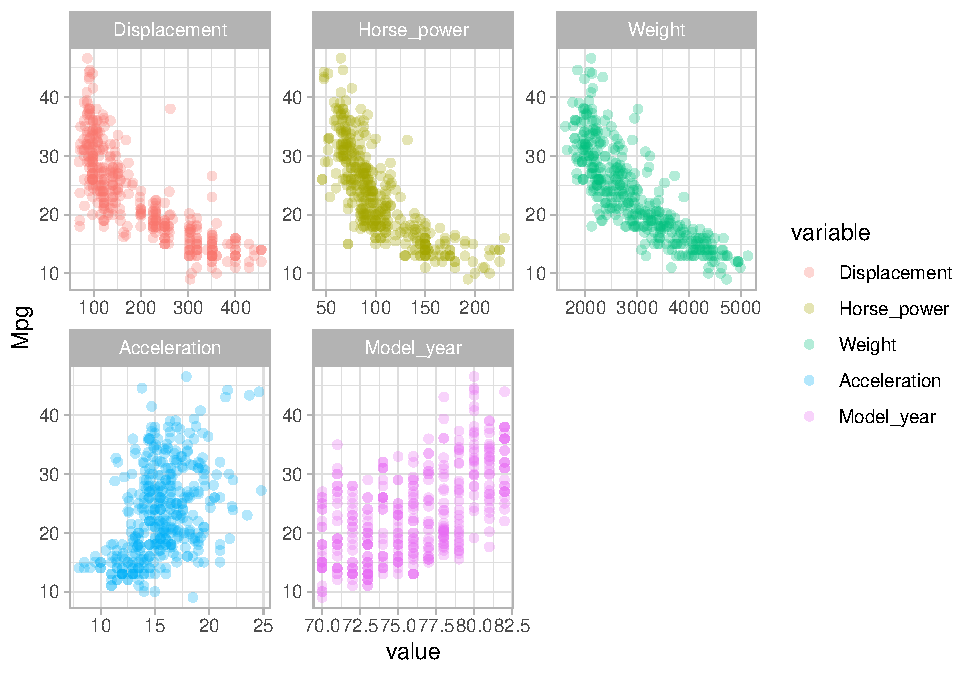
\includegraphics[width=.9\linewidth]{img/Regresion_files/figure-latex/unnamed-chunk-2-1} \caption{}\end{figure}

Como dijimos, se aprecia alta correlación entre Displacement, Horse\_power, Weight respecto de la salida, probablemente de forma logarítmica.

Las matrices de correlación nos confirmaban esta idea (con coeficientes de Pearson y Kendall)

\begin{figure}[H]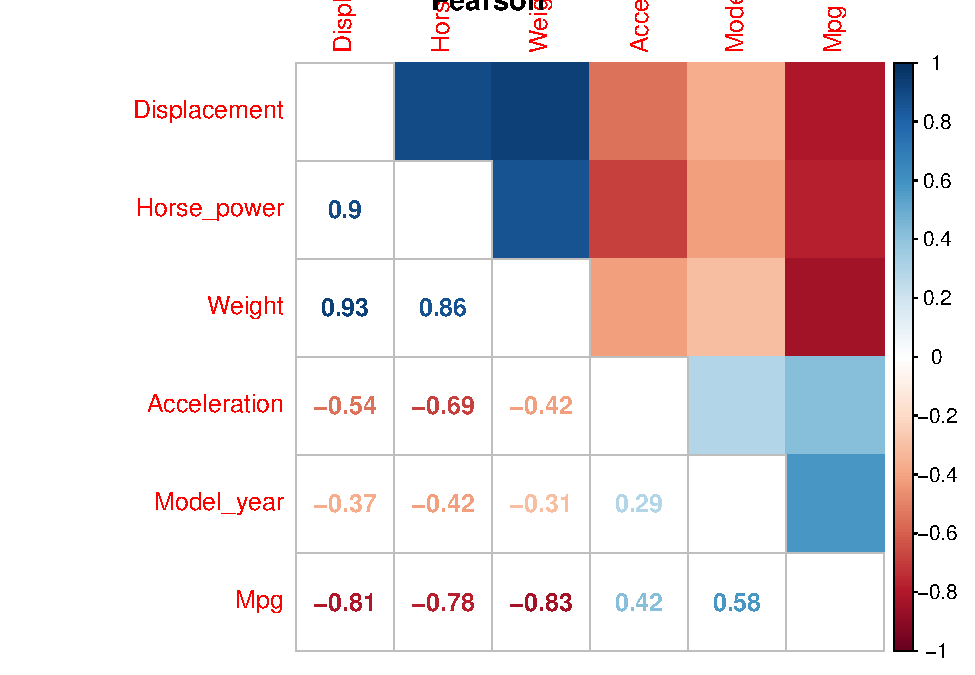
\includegraphics[width=.9\linewidth]{img/Regresion_files/figure-latex/unnamed-chunk-3-1} \caption{}\end{figure}

\begin{figure}[H]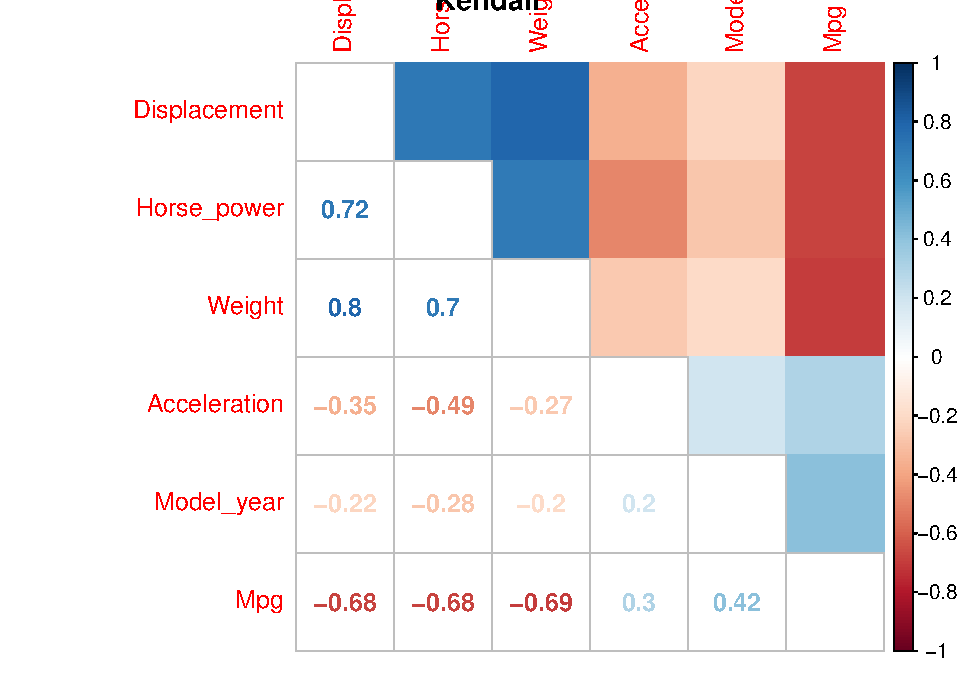
\includegraphics[width=.9\linewidth]{img/Regresion_files/figure-latex/unnamed-chunk-3-2} \caption{}\end{figure}

Por tanto, si las ordenáramos por cuáles parecen ser más prometedoras, tendríamos: Weight \textgreater{} Displacement \textgreater{} Horse\_power \textgreater{} Model\_year \textgreater{} Acceleration

También tenemos que tener en cuenta que las tres primeras variables están correladas entre sí.

\subsection{Ajustes de regresión lineal univariables}

Vamos a analizar un ajuste con cada una de las características:

\begin{verbatim}

Call: lm(formula = Mpg ~ Weight, data = auto)

Residuals:
     Min       1Q   Median       3Q      Max 
-11.9736  -2.7556  -0.3358   2.1379  16.5194 

Coefficients:
             Estimate Std. Error t value Pr(>|t|)    
(Intercept) 46.216524   0.798673   57.87   <2e-16 ***
Weight      -0.007647   0.000258  -29.64   <2e-16 ***
---
Signif. codes:  0 '***' 0.001 '**' 0.01 '*' 0.05 '.' 0.1 ' ' 1

Residual standard error: 4.333 on 390 degrees of freedom
Multiple R-squared:  0.6926,    Adjusted R-squared:  0.6918 
F-statistic: 878.8 on 1 and 390 DF,  p-value: < 2.2e-16

"-------------------------------------------"

Call: lm(formula = Mpg ~ Displacement, data = auto)

Residuals:
     Min       1Q   Median       3Q      Max 
-12.9170  -3.0243  -0.5021   2.3512  18.6128 

Coefficients:
             Estimate Std. Error t value Pr(>|t|)    
(Intercept)  35.12064    0.49443   71.03   <2e-16 ***
Displacement -0.06005    0.00224  -26.81   <2e-16 ***
---
Signif. codes:  0 '***' 0.001 '**' 0.01 '*' 0.05 '.' 0.1 ' ' 1

Residual standard error: 4.635 on 390 degrees of freedom
Multiple R-squared:  0.6482,    Adjusted R-squared:  0.6473 
F-statistic: 718.7 on 1 and 390 DF,  p-value: < 2.2e-16

"-------------------------------------------"

Call: lm(formula = Mpg ~ Horse_power, data = auto)

Residuals:
     Min       1Q   Median       3Q      Max 
-13.5710  -3.2592  -0.3435   2.7630  16.9240 

Coefficients:
             Estimate Std. Error t value Pr(>|t|)    
(Intercept) 39.935861   0.717499   55.66   <2e-16 ***
Horse_power -0.157845   0.006446  -24.49   <2e-16 ***
---
Signif. codes:  0 '***' 0.001 '**' 0.01 '*' 0.05 '.' 0.1 ' ' 1

Residual standard error: 4.906 on 390 degrees of freedom
Multiple R-squared:  0.6059,    Adjusted R-squared:  0.6049 
F-statistic: 599.7 on 1 and 390 DF,  p-value: < 2.2e-16

"-------------------------------------------"

Call: lm(formula = Mpg ~ Model_year, data = auto)

Residuals:
     Min       1Q   Median       3Q      Max 
-12.0212  -5.4411  -0.4412   4.9739  18.2088 

Coefficients:
             Estimate Std. Error t value Pr(>|t|)    
(Intercept) -70.01167    6.64516  -10.54   <2e-16 ***
Model_year    1.23004    0.08736   14.08   <2e-16 ***
---
Signif. codes:  0 '***' 0.001 '**' 0.01 '*' 0.05 '.' 0.1 ' ' 1

Residual standard error: 6.363 on 390 degrees of freedom
Multiple R-squared:  0.337, Adjusted R-squared:  0.3353 
F-statistic: 198.3 on 1 and 390 DF,  p-value: < 2.2e-16

"-------------------------------------------"

Call: lm(formula = Mpg ~ Acceleration, data = auto)

Residuals:
    Min      1Q  Median      3Q     Max 
-17.989  -5.616  -1.199   4.801  23.239 

Coefficients:
             Estimate Std. Error t value Pr(>|t|)    
(Intercept)    4.8332     2.0485   2.359   0.0188 *  
Acceleration   1.1976     0.1298   9.228   <2e-16 ***
---
Signif. codes:  0 '***' 0.001 '**' 0.01 '*' 0.05 '.' 0.1 ' ' 1

Residual standard error: 7.08 on 390 degrees of freedom
Multiple R-squared:  0.1792,    Adjusted R-squared:  0.1771 
F-statistic: 85.15 on 1 and 390 DF,  p-value: < 2.2e-16
\end{verbatim}

Al ser univariable, por ahora no es necesario fijarse en el estadístico F. Para ver el potencial de la variable, debemos darle importancia al p-valor (comprobar de que sea lo suficientemente bajo), y posteriormente ver el R\textsuperscript{2} para everiguar el porcentaje de la salida explicada.

\vspace{\baselineskip}

En base a los resultados vemos que el test de correlación nos había ayudado correctamente: de forma individual todas las variables tienen dependencia lineal, y el orden de calidad coincide con el orden de fuerza en las correlaciones.

Ya con el uso de la variable Weight vemos que podemos explicar un \textasciitilde69\% de la salida, un buen valor de partida. El ajuste quedaría de esta manera:

\begin{figure}[H]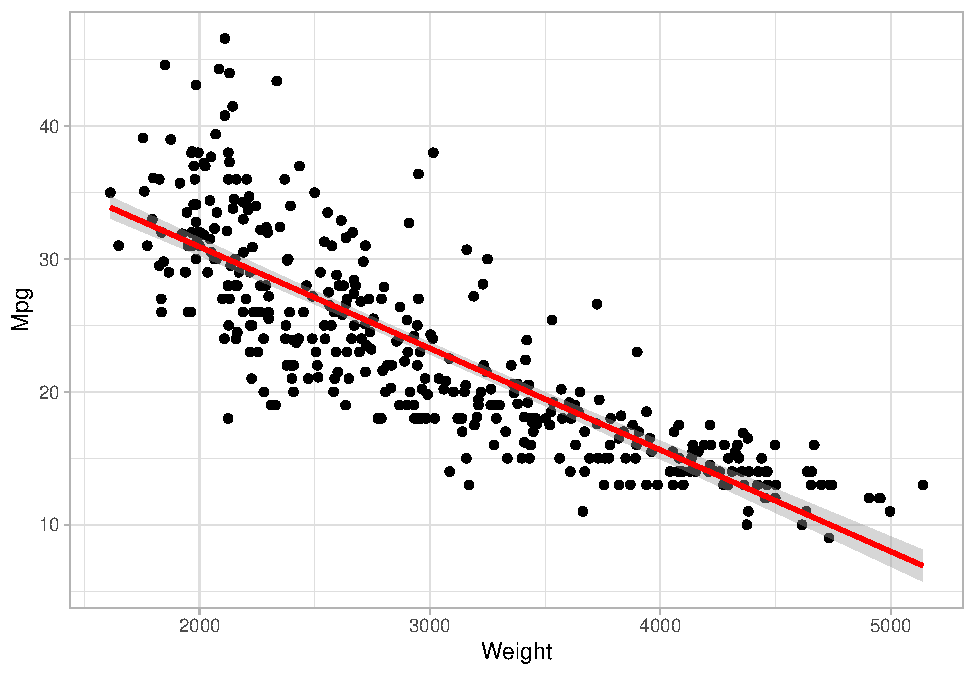
\includegraphics[width=.9\linewidth]{img/Regresion_files/figure-latex/unnamed-chunk-6-1} \caption{}\end{figure}

Con los coeficientes:

\begin{verbatim}
                   2.5 %      97.5 %
(Intercept) 44.646282308 47.78676679
Weight      -0.008154515 -0.00714017
\end{verbatim}

Aunque los valores del intervalo del coeficiente de Weight sea bajo, vemos que no incluye el cero (y con el p-valor obtenido anteriormente, lo podemos asegurar con bastante certeza). Probablemente la razón de estos coeficientes tan pequeños es que los datos no están estandarizados (se podría hacer perfectamente, se han dejado con sus rangos normales para interpretarlos mejor) y los valores de las unidades de medida son bastante diferentes (hablamos de rangos de {[}9.0,46.6{]} en Mpg frente a {[}1613,5140{]} en Weight)

\vspace{\baselineskip}

Ya con esto podemos intentan interpretar un poco los datos, tendríamos por ahora la fórmula de regresión lineal: 

\begin{equation}    
    Mpg \sim Weight
\end{equation}

\subsection{Ajustes de regresión lineal multivariable}

Aplicamos un método descendente:

\begin{verbatim}
Call: lm(formula = Mpg ~ ., data = auto)

Residuals:
    Min      1Q  Median      3Q     Max 
-8.5211 -2.3920 -0.1036  2.0312 14.2874 

Coefficients:
               Estimate Std. Error t value Pr(>|t|)    
(Intercept)  -1.544e+01  4.677e+00  -3.300  0.00106 ** 
Displacement  2.782e-03  5.462e-03   0.509  0.61082    
Horse_power   1.020e-03  1.376e-02   0.074  0.94095    
Weight       -6.874e-03  6.653e-04 -10.333  < 2e-16 ***
Acceleration  9.032e-02  1.019e-01   0.886  0.37599    
Model_year    7.541e-01  5.261e-02  14.334  < 2e-16 ***
---
Signif. codes:  0 '***' 0.001 '**' 0.01 '*' 0.05 '.' 0.1 ' ' 1

Residual standard error: 3.435 on 386 degrees of freedom
Multiple R-squared:  0.8088,    Adjusted R-squared:  0.8063 
F-statistic: 326.5 on 5 and 386 DF,  p-value: < 2.2e-16
\end{verbatim}

% \begin{center}\rule{\linewidth}{0.5pt}\end{center}

El p-valor del F estadístico nos dice que al menos hay una variable (realmente ya lo sabíamos de los ajustes univariables) con dependencia linea.

\vspace{\baselineskip}

Vemos que hay 3 variables con mal p-valor, empezamos quitando la que lo tiene más alto, Horse\_power.

\begin{center}\rule{\linewidth}{0.5pt}\end{center}

\begin{verbatim}
Call: lm(formula = Mpg ~ . - Horse_power, data = auto)

Residuals:
    Min      1Q  Median      3Q     Max 
-8.5182 -2.3948 -0.1085  2.0405 14.2908 

Coefficients:
               Estimate Std. Error t value Pr(>|t|)    
(Intercept)  -1.527e+01  4.106e+00  -3.719 0.000229 ***
Displacement  2.874e-03  5.310e-03   0.541 0.588651    
Weight       -6.852e-03  5.967e-04 -11.483  < 2e-16 ***
Acceleration  8.555e-02  7.885e-02   1.085 0.278595    
Model_year    7.532e-01  5.118e-02  14.717  < 2e-16 ***
---
Signif. codes:  0 '***' 0.001 '**' 0.01 '*' 0.05 '.' 0.1 ' ' 1

Residual standard error: 3.431 on 387 degrees of freedom
Multiple R-squared:  0.8088,    Adjusted R-squared:  0.8068 
F-statistic: 409.2 on 4 and 387 DF,  p-value: < 2.2e-16
\end{verbatim}

El F estadístico está correcto, y seguimos teniendo variables con p-valor grande, quitamos Displacement.

\begin{center}\rule{\linewidth}{0.5pt}\end{center}

\begin{verbatim}
Call: lm(formula = Mpg ~ . - Horse_power - Displacement, data = auto)

Residuals:
    Min      1Q  Median      3Q     Max 
-8.6749 -2.3528 -0.1082  2.0168 14.3022 

Coefficients:
               Estimate Std. Error t value Pr(>|t|)    
(Intercept)  -14.936555   4.055512  -3.683 0.000263 ***
Weight        -0.006554   0.000230 -28.502  < 2e-16 ***
Acceleration   0.066359   0.070361   0.943 0.346204    
Model_year     0.748446   0.050366  14.860  < 2e-16 ***
---
Signif. codes:  0 '***' 0.001 '**' 0.01 '*' 0.05 '.' 0.1 ' ' 1

Residual standard error: 3.428 on 388 degrees of freedom
Multiple R-squared:  0.8086,    Adjusted R-squared:  0.8071 
F-statistic: 546.5 on 3 and 388 DF,  p-value: < 2.2e-16
\end{verbatim}

\textit{idem}. a lo anterior, quitamos Acceleration.

\begin{center}\rule{\linewidth}{0.5pt}\end{center}

\begin{verbatim}
Call: lm(formula = Mpg ~ . - Horse_power - Displacement - Acceleration, 
    data = auto)

Residuals:
    Min      1Q  Median      3Q     Max 
-8.8505 -2.3014 -0.1167  2.0367 14.3555 

Coefficients:
              Estimate Std. Error t value Pr(>|t|)    
(Intercept) -1.435e+01  4.007e+00  -3.581 0.000386 ***
Weight      -6.632e-03  2.146e-04 -30.911  < 2e-16 ***
Model_year   7.573e-01  4.947e-02  15.308  < 2e-16 ***
---
Signif. codes:  0 '***' 0.001 '**' 0.01 '*' 0.05 '.' 0.1 ' ' 1

Residual standard error: 3.427 on 389 degrees of freedom
Multiple R-squared:  0.8082,    Adjusted R-squared:  0.8072 
F-statistic: 819.5 on 2 and 389 DF,  p-value: < 2.2e-16
\end{verbatim}

El estadístico F sigue bien, y los p-valores de las variables son extremadamente bajos. Nos fijamos en el R\textsuperscript{2} y vemos que ha subido considerablemente (un 10\%) respecto al univariable, por lo que este sería nuestro modelo aditivo por ahora.

\vspace{\baselineskip}

A partir de ahora deberíamos tener cuidado si el R\textsuperscript{2} sigue aumentando, hay que evitar el overfitting en el modelo.

\subsection{Inserción de interacciones}

Del modelo aditivo solo nos han quedado dos regresores, así que probamos a incluirlos como interacción.

\begin{verbatim}
Call: lm(formula = Mpg ~ +Weight * Model_year, data = auto)

Residuals:
    Min      1Q  Median      3Q     Max 
-8.0397 -1.9956 -0.0983  1.6525 12.9896 

Coefficients:
                    Estimate Std. Error t value Pr(>|t|)    
(Intercept)       -1.105e+02  1.295e+01  -8.531 3.30e-16 ***
Weight             2.755e-02  4.413e-03   6.242 1.14e-09 ***
Model_year         2.040e+00  1.718e-01  11.876  < 2e-16 ***
Weight:Model_year -4.579e-04  5.907e-05  -7.752 8.02e-14 ***
---
Signif. codes:  0 '***' 0.001 '**' 0.01 '*' 0.05 '.' 0.1 ' ' 1

Residual standard error: 3.193 on 388 degrees of freedom
Multiple R-squared:  0.8339,    Adjusted R-squared:  0.8326 
F-statistic: 649.3 on 3 and 388 DF,  p-value: < 2.2e-16
\end{verbatim}

El F estadístico sigue bien y los p-valores son bajos, el nuevo R\textsuperscript{2} ha mejorado un 3\%, así que no es demasiado para considerar un overfitting. Probablemente más de un 90\% sería preocupante, pero también tenemos que tener en cuenta que las variables están fuertemente correladas con la salida.

\vspace{\baselineskip}

Podríamos probar a añadir alguna interacción más con alguna variable que no hubiera entrado en el modelo aditivo, pero no se espera que mejore:

\begin{center}\rule{\linewidth}{0.5pt}\end{center}

\begin{verbatim}
Call: lm(formula = Mpg ~ +Weight * Model_year + Acceleration * Displacement, 
    data = auto)

Residuals:
    Min      1Q  Median      3Q     Max 
-7.3130 -1.8670 -0.0426  1.6109 12.2499 

Coefficients:
                            Estimate Std. Error t value Pr(>|t|)    
(Intercept)               -1.131e+02  1.321e+01  -8.564 2.65e-16 ***
Weight                     2.456e-02  4.693e-03   5.234 2.73e-07 ***
Model_year                 1.907e+00  1.769e-01  10.778  < 2e-16 ***
Acceleration               7.273e-01  1.282e-01   5.671 2.79e-08 ***
Displacement               3.605e-02  8.673e-03   4.157 3.98e-05 ***
Weight:Model_year         -4.054e-04  6.281e-05  -6.454 3.29e-10 ***
Acceleration:Displacement -2.953e-03  6.219e-04  -4.748 2.91e-06 ***
---
Signif. codes:  0 '***' 0.001 '**' 0.01 '*' 0.05 '.' 0.1 ' ' 1

Residual standard error: 3.075 on 385 degrees of freedom
Multiple R-squared:  0.8472,    Adjusted R-squared:  0.8448 
F-statistic: 355.7 on 6 and 385 DF,  p-value: < 2.2e-16
\end{verbatim}

A pesar de nuestra suposición los p-valores son válidos y el R\textsuperscript{2} aumenta un 1\%. Es cuestionable si el aumento de la complejidad del modelo merece con este incremento de R\textsuperscript{2}. Por simplificar vamos a quedarnos con el modelo aditivo anterior y probar con otra interacción.

\vspace{\baselineskip}

Podemos probar combinando la variable Acceleration separadamente con las que ya teníamos (Weight y Model\_year).

\begin{center}\rule{\linewidth}{0.5pt}\end{center}

\begin{verbatim}

Call: lm(formula = Mpg ~ +Weight * Model_year + Acceleration * Weight, 
    data = auto)

Residuals:
    Min      1Q  Median      3Q     Max 
-7.4473 -1.7994 -0.0496  1.4790 12.1258 

Coefficients:
                      Estimate Std. Error t value Pr(>|t|)    
(Intercept)         -1.230e+02  1.298e+01  -9.480  < 2e-16 ***
Weight               2.971e-02  4.419e-03   6.722 6.47e-11 ***
Model_year           1.926e+00  1.742e-01  11.055  < 2e-16 ***
Acceleration         1.341e+00  2.323e-01   5.772 1.61e-08 ***
Weight:Model_year   -4.078e-04  6.197e-05  -6.581 1.53e-10 ***
Weight:Acceleration -3.808e-04  7.537e-05  -5.052 6.76e-07 ***
---
Signif. codes:  0 '***' 0.001 '**' 0.01 '*' 0.05 '.' 0.1 ' ' 1

Residual standard error: 3.061 on 386 degrees of freedom
Multiple R-squared:  0.8482,    Adjusted R-squared:  0.8462 
F-statistic: 431.4 on 5 and 386 DF,  p-value: < 2.2e-16
\end{verbatim}

\begin{center}\rule{\linewidth}{0.5pt}\end{center}

\begin{verbatim}
Call: lm(formula = Mpg ~ +Weight * Model_year + Acceleration * Model_year, 
    data = auto)

Residuals:
    Min      1Q  Median      3Q     Max 
-7.8674 -1.9539 -0.0617  1.7397 12.3964 

Coefficients:
                          Estimate Std. Error t value Pr(>|t|)    
(Intercept)             -4.046e+01  2.833e+01  -1.428  0.15401    
Weight                   2.523e-02  4.881e-03   5.170 3.76e-07 ***
Model_year               1.072e+00  3.704e-01   2.895  0.00401 ** 
Acceleration            -3.956e+00  1.268e+00  -3.120  0.00195 ** 
Weight:Model_year       -4.263e-04  6.475e-05  -6.584 1.49e-10 ***
Model_year:Acceleration  5.476e-02  1.663e-02   3.293  0.00108 ** 
---
Signif. codes:  0 '***' 0.001 '**' 0.01 '*' 0.05 '.' 0.1 ' ' 1

Residual standard error: 3.117 on 386 degrees of freedom
Multiple R-squared:  0.8426,    Adjusted R-squared:  0.8406 
F-statistic: 413.2 on 5 and 386 DF,  p-value: < 2.2e-16
\end{verbatim}

Y entre los dos nos podríamos quedar con el primero por tener mejores p-valores y un mejor R\textsuperscript{2}. Aun así, el incremento es pequeño respecto a nuestro modelo aditivo.

\vspace{\baselineskip}

La fórmula del modelo aditivo que llevamos por ahora es:
\begin{equation}
    Mpg \sim Weight + Model_year + Acceleration + Weight*Model_year + Weight*Acceleration
\end{equation}

Gráficamente:
\begin{figure}[H]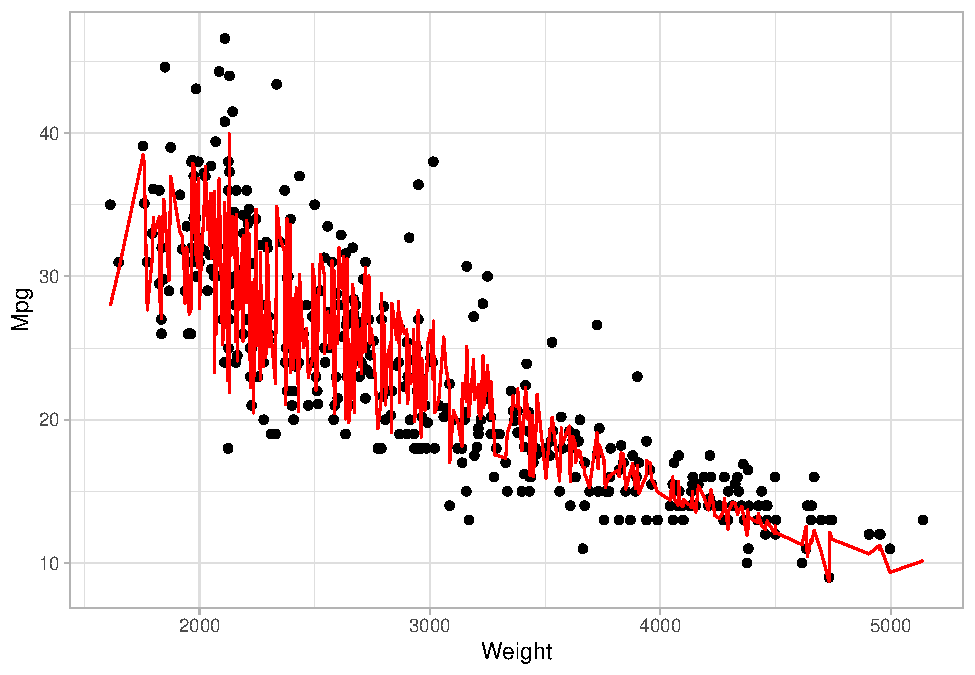
\includegraphics[width=.9\linewidth]{img/Regresion_files/figure-latex/unnamed-chunk-16-1} \caption{}\end{figure}

Por el uso multivariable la línea de regresión que se forma podría indicarnos un posible overfitting en el modelo, vamos a dejarlo por ahora e intentar solucionarlo con el modelo no lineal.

\subsection{Ajustes de regresión no lineal}

Habíamos dicho que las gráficas nos mostraban una tendencia logarítmica, vamos a incluír la de Weight en nuestro modelo aditivo:
\begin{verbatim}
Call: lm(formula = Mpg ~ +Weight * Model_year + Acceleration * Weight + 
    I(log(Weight)), data = auto)

Residuals:
    Min      1Q  Median      3Q     Max 
-7.6734 -1.7933 -0.0576  1.3154 12.1716 

Coefficients:
                      Estimate Std. Error t value Pr(>|t|)    
(Intercept)          1.191e+02  4.120e+01   2.891  0.00406 ** 
Weight               2.842e-02  4.227e-03   6.723 6.44e-11 ***
Model_year           1.638e+00  1.728e-01   9.480  < 2e-16 ***
Acceleration         7.236e-01  2.435e-01   2.972  0.00315 ** 
I(log(Weight))      -3.028e+01  4.914e+00  -6.162 1.81e-09 ***
Weight:Model_year   -2.971e-04  6.186e-05  -4.803 2.24e-06 ***
Weight:Acceleration -1.775e-04  7.919e-05  -2.241  0.02559 *  
---
Signif. codes:  0 '***' 0.001 '**' 0.01 '*' 0.05 '.' 0.1 ' ' 1

Residual standard error: 2.924 on 385 degrees of freedom
Multiple R-squared:  0.8618,    Adjusted R-squared:  0.8597 
F-statistic: 400.2 on 6 and 385 DF,  p-value: < 2.2e-16
\end{verbatim}

El estadístico F está bien y los p-valores también, aunque el de la interacción Weight-Acceleration es alto comparado con el resto (aún así sigue siendo aceptable).

Como el R\textsuperscript{2} ha subido, por ver si mejora, vamos a quitar esta interacción.

\begin{center}\rule{\linewidth}{0.5pt}\end{center}

\begin{verbatim}
Call: lm(formula = Mpg ~ +Weight * Model_year + I(log(Weight)), data = auto)

Residuals:
    Min      1Q  Median      3Q     Max 
-8.7501 -1.7470 -0.0725  1.3122 12.6776 

Coefficients:
                    Estimate Std. Error t value Pr(>|t|)    
(Intercept)        1.715e+02  3.810e+01   4.501 8.98e-06 ***
Weight             2.522e-02  4.119e-03   6.123 2.25e-09 ***
Model_year         1.572e+00  1.708e-01   9.202  < 2e-16 ***
I(log(Weight))    -3.540e+01  4.538e+00  -7.800 5.82e-14 ***
Weight:Model_year -2.701e-04  6.003e-05  -4.499 9.04e-06 ***
---
Signif. codes:  0 '***' 0.001 '**' 0.01 '*' 0.05 '.' 0.1 ' ' 1

Residual standard error: 2.972 on 387 degrees of freedom
Multiple R-squared:  0.8565,    Adjusted R-squared:  0.855 
F-statistic: 577.3 on 4 and 387 DF,  p-value: < 2.2e-16
\end{verbatim}

Hemos empeorado un 0.5\%, bastante poco, y el modelo es más simple. La dejamos quitada.

Mostramos este ajuste:
\begin{figure}[H]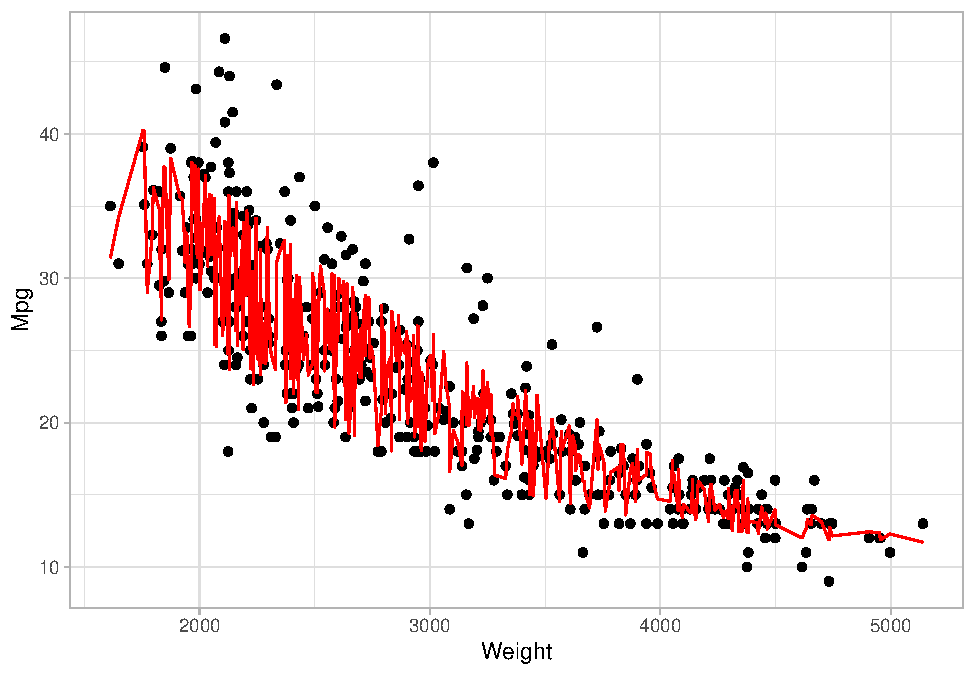
\includegraphics[width=.9\linewidth]{img/Regresion_files/figure-latex/unnamed-chunk-19-1} \caption{}\end{figure}

Esta gráfica nos indica que es probable que se esté generando sobreajuste, se ve necesario simplificar el modelo.

\begin{center}\rule{\linewidth}{0.5pt}\end{center}

Si quitamos la otra interacción:
\begin{verbatim}

Call: lm(formula = Mpg ~ Weight + Model_year + I(log(Weight)), data = auto)

Residuals:
    Min      1Q  Median      3Q     Max 
-9.3384 -1.7476 -0.2122  1.5322 13.2812 

Coefficients:
                 Estimate Std. Error t value Pr(>|t|)    
(Intercept)    284.287315  29.392946   9.672  < 2e-16 ***
Weight           0.007772   0.001420   5.473 7.97e-08 ***
Model_year       0.828693   0.044506  18.620  < 2e-16 ***
I(log(Weight)) -43.590633   4.258803 -10.235  < 2e-16 ***
---
Signif. codes:  0 '***' 0.001 '**' 0.01 '*' 0.05 '.' 0.1 ' ' 1

Residual standard error: 3.045 on 388 degrees of freedom
Multiple R-squared:  0.849, Adjusted R-squared:  0.8478 
F-statistic:   727 on 3 and 388 DF,  p-value: < 2.2e-16
\end{verbatim}

No hemos perdido apenas R\textsuperscript{2}. Mostramos la gráfica:

\begin{figure}[H]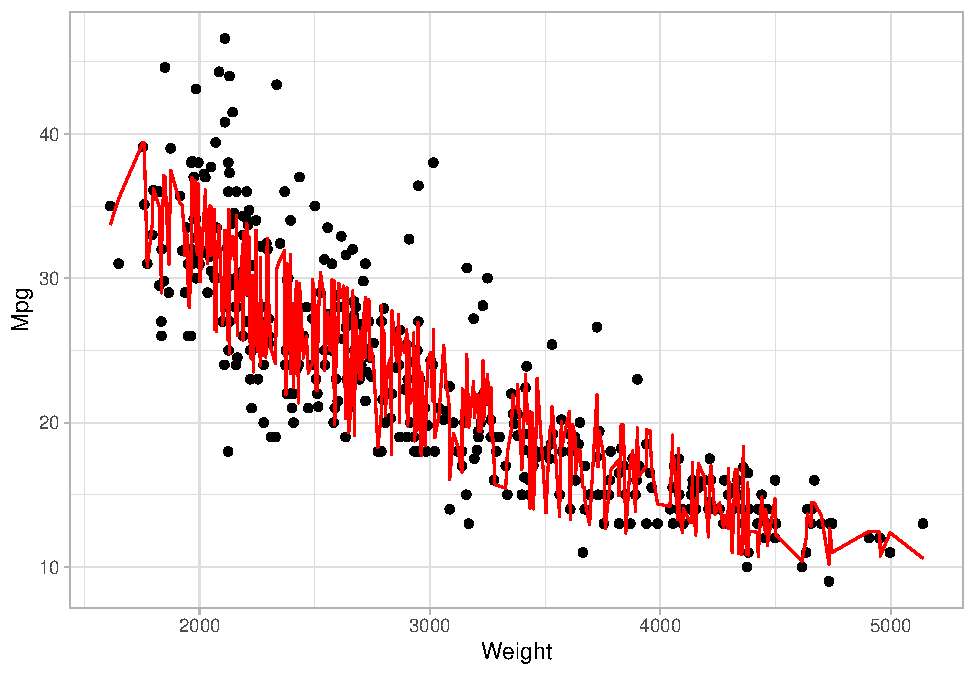
\includegraphics[width=.9\linewidth]{img/Regresion_files/figure-latex/unnamed-chunk-21-1} \caption{}\end{figure}

Seguimos con el mismo problema, probablemente se deba a una de las variables. Quitamos Model\_year por tener poca correlación con la variable de salida:

\begin{verbatim}
Call: lm(formula = Mpg ~ Weight + I(log(Weight)), data = auto)

Residuals:
     Min       1Q   Median       3Q      Max 
-12.5329  -2.7031  -0.4016   1.7038  16.0835 

Coefficients:
                 Estimate Std. Error t value Pr(>|t|)    
(Intercept)    263.812407  40.366256   6.535 1.99e-10 ***
Weight           0.002582   0.001914   1.349    0.178    
I(log(Weight)) -31.166013   5.780558  -5.392 1.21e-07 ***
---
Signif. codes:  0 '***' 0.001 '**' 0.01 '*' 0.05 '.' 0.1 ' ' 1

Residual standard error: 4.185 on 389 degrees of freedom
Multiple R-squared:  0.714, Adjusted R-squared:  0.7125 
F-statistic: 485.6 on 2 and 389 DF,  p-value: < 2.2e-16
\end{verbatim}

El p-valor de Weight nos indica que hay que quitarla, y al no estar incluída ninguna interacción, no es un término de jerarquía, por lo que podemos hacerlo. Se puede porque la variable sigue siendo independiente, solamente no está modelada de forma lineal, sino logarítmicamente.

\begin{verbatim}
Call: lm(formula = Mpg ~ I(log(Weight)), data = auto)

Residuals:
     Min       1Q   Median       3Q      Max 
-12.4315  -2.6752  -0.2888   1.9429  16.0136 

Coefficients:
               Estimate Std. Error t value Pr(>|t|)    
(Intercept)    209.9433     6.0002   34.99   <2e-16 ***
I(log(Weight)) -23.4317     0.7534  -31.10   <2e-16 ***
---
Signif. codes:  0 '***' 0.001 '**' 0.01 '*' 0.05 '.' 0.1 ' ' 1

Residual standard error: 4.189 on 390 degrees of freedom
Multiple R-squared:  0.7127,    Adjusted R-squared:  0.7119 
F-statistic: 967.3 on 1 and 390 DF,  p-value: < 2.2e-16
\end{verbatim}

\begin{figure}[H]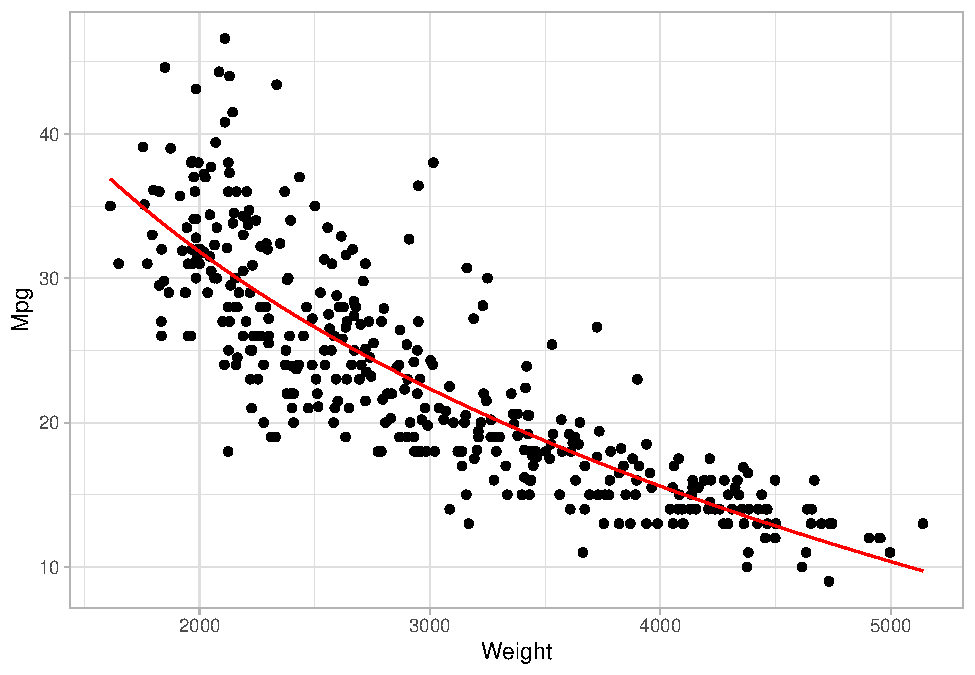
\includegraphics[width=.9\linewidth]{img/Regresion_files/figure-latex/unnamed-chunk-24-1} \caption{}\end{figure}

\begin{figure}[H]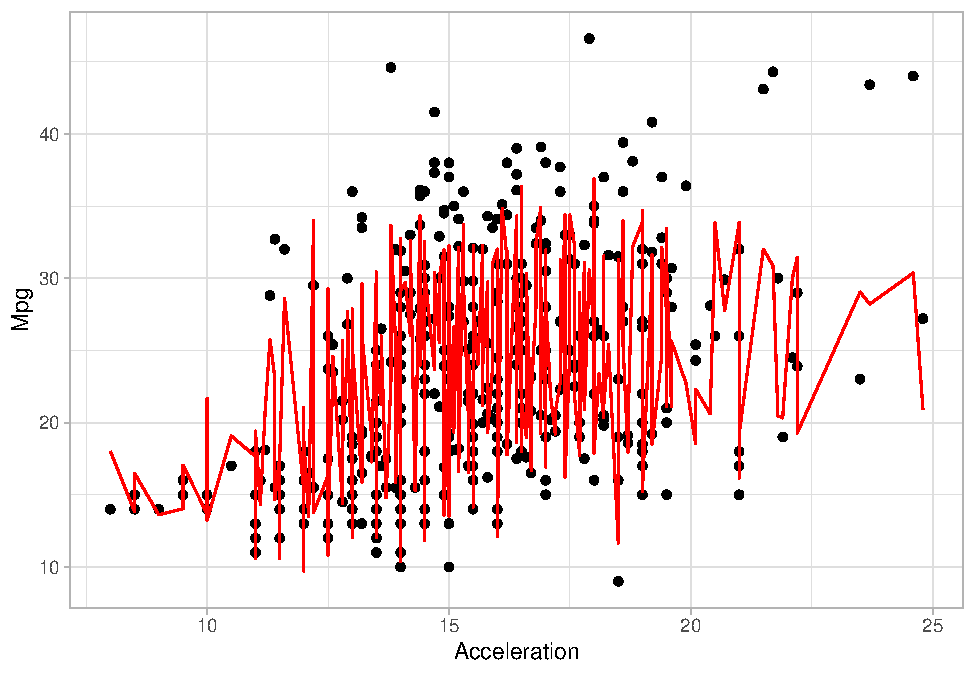
\includegraphics[width=.9\linewidth]{img/Regresion_files/figure-latex/unnamed-chunk-24-2} \caption{}\end{figure}

\begin{figure}[H]\includegraphics[width=.9\linewidth]{img/Regresion_files/figure-latex/unnamed-chunk-24-3} \caption{}\end{figure}

Vemos un empeoramiento significativo en la calidad de R\textsuperscript{2} respecto al modelo multivariable, pero la forma del modelo no está tan ajustada a los datos y parece sensato mantenerlo así.

Aún así, no resulta lógico intentar predecir el Mpg de un coche únicamente en base al peso, alguna de las otras variables deberían ayudarnos en la predicción. Por ejemplo, alguna característica del motor, como la cilindrada o los caballos de vapor.

\vspace{\baselineskip}

Para resumir, mostramos el modelo con mejor R\textsuperscript{2} tras hacer múltiples pruebas, e intentando evitar un overfitting:
\begin{verbatim}
Call: lm(formula = Mpg ~ Acceleration + I(log(Weight)) + I(log(Displacement)), 
    data = auto)

Residuals:
     Min       1Q   Median       3Q      Max 
-12.9074  -2.6174  -0.4104   1.9500  16.5596 

Coefficients:
                      Estimate Std. Error t value Pr(>|t|)    
(Intercept)          171.61778   12.14751  14.128  < 2e-16 ***
Acceleration           0.19717    0.08914   2.212   0.0276 *  
I(log(Weight))       -16.94003    2.27727  -7.439 6.59e-13 ***
I(log(Displacement))  -3.19963    1.26881  -2.522   0.0121 *  
---
Signif. codes:  0 '***' 0.001 '**' 0.01 '*' 0.05 '.' 0.1 ' ' 1

Residual standard error: 4.104 on 388 degrees of freedom
Multiple R-squared:  0.7256,    Adjusted R-squared:  0.7235 
F-statistic: 342.1 on 3 and 388 DF,  p-value: < 2.2e-16
\end{verbatim}

Los p-valores no son muy fuertes, pero siguen siendo aceptables, y gráficamente el modelo se ve un poco mejor:
\begin{figure}[H]\includegraphics[width=.9\linewidth]{img/Regresion_files/figure-latex/unnamed-chunk-26-1} \caption{}\end{figure}

\begin{figure}[H]\includegraphics[width=.9\linewidth]{img/Regresion_files/figure-latex/unnamed-chunk-26-2} \caption{}\end{figure}

\begin{figure}[H]\includegraphics[width=.9\linewidth]{img/Regresion_files/figure-latex/unnamed-chunk-26-3} \caption{}\end{figure}

Pensando en el problema, y tras el análisis hecho en el apartado de EDA, creemos que usar Model\_year para predecir Mpg no parece buena idea. La gráfica de la variable nos muestra mucha dispersión en los datos y, aunque sí se ve un cierta tendencia lineal, no parece suficiente para usarla. Claramente nos ajusta mejor los datos pero parece que nos estamos pegando a ellos.

De cara a comprobar este razonamiento en el cross-validation, vamos a guardar dos modelos: 

\vspace{\baselineskip}
Modelo con mejor R\textsuperscript{2} 

\begin{equation}    
    Mpg \sim Weight + Model\_year + I(log(Weight)
\end{equation}

Modelo intentando evitar el overfitting
\begin{equation}    
    Mpg \sim Acceleration + I(log(Weight)) + I(log(Displacement))
\end{equation}

\subsection{Ajustes con KNN}

Sabemos que la función por defecto usa la distancia de Minkowski y escala los datos a igual rango. También usa un K de 7, pero sería recomendable probar con varios.

\vspace{\baselineskip}

Vamos a probar con diferentes modelos, primero el multivariable con todas
\begin{verbatim}
Mpg ~ .
    1.880835
\end{verbatim}

Y probando con varios obtenemos el menor error eliminando únicamente Acceleration:
\begin{verbatim}
Mpg ~ . - Acceleration    
    1.856269
\end{verbatim}

Que visualmente nos quedaría:
\begin{figure}[H]\includegraphics[width=.9\linewidth]{img/Regresion_files/figure-latex/unnamed-chunk-29-1} \caption{}\end{figure}

\begin{figure}[H]\includegraphics[width=.9\linewidth]{img/Regresion_files/figure-latex/unnamed-chunk-29-2} \caption{}\end{figure}

Si probamos el modelo no lineal obtenido en los pasos anteriores (con mejor R\textsuperscript{2}) nos un error bastante malo.
\begin{verbatim}
Mpg ~ Weight + Model_year + I(log(Weight))
    2.104086
\end{verbatim}

\vspace{\baselineskip}

El método para evitar el overfitting que usamos en el apartado anterior probablemente no funcione con KNN por seguir una metodología totalmente diferente. El ajuste de KNN para regresión no tiene nada que ver con los modelos LM. Podemos aún así comprobarlo:
\begin{verbatim}
Mpg ~ Acceleration + I(log(Weight)
    2.938051
\end{verbatim}

Gráficamente este quedaría de la siguiente manera:
\begin{figure}[H]\includegraphics[width=.9\linewidth]{img/Regresion_files/figure-latex/unnamed-chunk-32-1} \caption{}\end{figure}

\begin{figure}[H]\includegraphics[width=.9\linewidth]{img/Regresion_files/figure-latex/unnamed-chunk-32-2} \caption{}\end{figure}

Por completitud, podríamos usarlo también en cross-validation para comprobarlo con un conjunto de test.

\vspace{\baselineskip}

Tendríamos por tanto los siguientes modelos para KNN: 
\begin{equation}
    Mpg \sim . - Acceleration 
\end{equation}

\begin{equation}    
    Mpg \sim Acceleration + I(log(Weight)) + I(log(Displacement))
\end{equation}

\vspace{\baselineskip}

Comparándolos gráficamente vemos que son similares, aunque el que intenta evitar el overfitting (en color azul en la gráfica), tiene menor dispersión:
\begin{figure}[H]\includegraphics[width=.9\linewidth]{img/Regresion_files/figure-latex/unnamed-chunk-33-1} \caption{}\end{figure}

\begin{figure}[H]\includegraphics[width=.9\linewidth]{img/Regresion_files/figure-latex/unnamed-chunk-33-2} \caption{}\end{figure}

\subsection{Comparativa de los ajustes anteriores con cross-validation}

Recordamos los modelos obtenidos.

\vspace{\baselineskip}
LM: 
\begin{equation}
    Mpg \sim Weight + Model\_year + I(log(Weight)
\end{equation}
\begin{equation}    
    Mpg \sim Acceleration + I(log(Weight)) + I(log(Displacement))
\end{equation}

\vspace{\baselineskip}
KNN: 
\begin{equation}    
    Mpg \sim . - Acceleration
\end{equation}

\begin{equation}    
    Mpg \sim Acceleration + I(log(Weight)) + I(log(Displacement))
\end{equation}

\vspace{\baselineskip}

Con el proceso de cross-validation dividimos el dataset en N subconjuntos (folds) y repetimos el entrenamiento N veces. Cada entrenamiento se aplica reservando uno de los subconjuntos como test y entrenando con el resto. Al final, el error obtenido para el modelo es la media de los errores en cada fold. La elección del número de folds es importante y si el problema lo permite (en términos de gasto computacional), se debería probar con varios. En este caso hemos utilizado 5 folds.

Con esto conseguimos no desperdiciar el conocimiento del conjunto de test y no guiarnos por una única evaluación del modelo.

\vspace{\baselineskip}

Aplicando este proceso obtenemos los siguiente:
\begin{verbatim}
Regresión 1:  9.333066
Regresión 2: 17.10519
KNN 1:        7.291517
KNN 2:       18.43846
\end{verbatim}

Los resultados nos muestra que los modelos con los que obtuvimos mejores valores de R\textsuperscript{2} y RSME en sus apartados han acabado con mejor RSME tras el cross-validation. También apreciamos que con KNN conseguimos ligeramente mejores resultados que regresión lineal/no-lineal.

\vspace{\baselineskip}

Por completitud, mostramos también los resultados en training:
\begin{verbatim}
Regresión 1:  9.159891
Regresión 2: 16.62285
KNN 1:        3.659828
KNN 2:        8.642349
\end{verbatim}

Que nos muestran que ninguno de los modelos LM estaba haciendo overfitting. 
Adicionalmente, en KNN existe una diferencia significativa entre training y test.

\subsection{Comparativa de tests}

Para comparar los algoritmos vamos a aplicar test estadísticos en base a los resultados obtenidos en múltiples datasets. Para asegurar la igualdad de condiciones los algoritmos hacen uso de parámetros genéricos y utilizan las mismas particiones de cross-validation.

\vspace{\baselineskip}

Estas son las tablas de resultados que tenemos para test:
\begin{longtable}[]{@{}rr@{}}
\toprule
out\_test\_lm & out\_test\_kknn\tabularnewline
\midrule
\endhead
0.1909091 & 0.1000000\tabularnewline
0.1000000 & 1.0294118\tabularnewline
0.1000000 & 0.4339071\tabularnewline
0.1000000 & 0.3885965\tabularnewline
0.1548506 & 0.1000000\tabularnewline
0.1000000 & 0.3061057\tabularnewline
\bottomrule
\end{longtable}

\vspace{\baselineskip}

Aplicamos el test de Wilconxon a LM y KNN:
\begin{verbatim}
 V    V
78 - 93 

p-value:  0.7660294
\end{verbatim}

Obtenemos un ranking de 78 para LM y 93 para KNN, con un p-valor de 0.77 (o nivel de confianza del 33\%).

Esto nos dice que gana KNN pero puesto que el p-value no es lo suficientemente grande no podemos afirmar con un nivel alto de significación que las diferencias entre los tests sean notorias.

\vspace{\baselineskip}

Ahora aplicamos en test de Friedman a los dos algoritmos anteriores junto al algoritmo M5:
\begin{verbatim}
Friedman rank sum test

data:  as.matrix(tablatst)
Friedman chi-squared = 8.4444, df = 2, p-value = 0.01467
\end{verbatim}

El p-value es \textless0.05 por lo que podemos concluir que al menos hay un par de algoritmos de calidad diferente.

\vspace{\baselineskip}

Vemos cuáles de ellos lo son haciendo el test post-hoc de HOLM
\begin{verbatim}
Pairwise comparisons using Wilcoxon signed rank exact test 

data:  as.matrix(tablatst) and groups 

  1     2    
2 0.580 -    
3 0.081 0.108

P value adjustment method: holm 
\end{verbatim}

Con el test post-hoc de HOLM podemos asegurar que 3-1 (M5 vs LM) son diferentes. También podemos afirmar M5 respecto de KNN pero con un nivel de confianza menor.

\vspace{\baselineskip}

De KNN y LM no podemos afirmar nada puesto que el p-valor es extremadamente grande. \newpage
    \section{Clasificación: Análisis Estadístico de Datos}

\subsection{Introducción}

Para el problema de clasificación hacemos uso del dataset \textbf{haberman} \cite{haberman}, que codifica el ratio de supervivencia de pacientes operados de cáncer de pecho en el Hospital Universitario de Chicago, en base a las siguientes características:

\begin{enumerate}
\def\labelenumi{\arabic{enumi}.}
    \item \textbf{Age}: Indica la edad del paciente en el momento de la operación.
    \item \textbf{Year}: Los dos últimas cifras del año en el que se operó el paciente.
    \item \textbf{Positive}: Número de nodos auxiliares positivos detectados. Esta variable hace referencia a los ganglios linfáticos que dan positivos como presentes de cáncer. A mayor número de nodos detectados, mayor es la gravedad del cáncer. 
    
    Aunque normalmente la primera zona de propagación del cáncer son estos nodos, no es la única medida de la seriedad, pues este puede propagarse a otras zonas del cuerpo. En principio no deberíamos descartar la posibilidad de que puede haber casos de no supervivencia con bajo número de positivos.

    Viendo que solo tenemos esta medida del cáncer en el dataset es posible que la operación que recibieron los pacientes sea algún tipo de cirugía de ganglios linfáticos, donde el cirujano intenta extraer los nodos afectados por el tumor. Por consiguiente, cuanto mayor es la cantidad de nodos detectados, más complicaciones pueden acarrearse de la operación \cite{cancer1, cancer2}.
\end{enumerate}

El objetivo es poder clasificar, en base a los tres atributos, si los pacientes pueden sobrevivir 5 años o más:

\begin{enumerate}
    \def\labelenumi{\arabic{enumi}.}
    \setcounter{enumi}{3}
    \item \textbf{Survival}: Sí/No indicando la supervivencia del paciente tras 5 años.
\end{enumerate}

Contamos por tanto con un problema de clasificación binario en base a tres características, y con un número total de 306 instancias.

\vspace{\baselineskip}

La descripción del problema nos da alguna información adicional sobre las variables:

\begin{enumerate}
    \def\labelenumi{\arabic{enumi}.}
    \item \textbf{Age}: Variable numérica discreta, contamos con valores enteros en el
    rango {[}30,83{]}.
    \item \textbf{Year}: Variable numérica discreta, contamos con valores enteros en el
    rango {[}58,69{]}.
    \item \textbf{Positive}: Variable numérica discreta, contamos con valores enteros en
    el rango {[}0,52{]}.
    \item \textbf{Survival}: Variable binaria.
\end{enumerate}

\paragraph{Hipótesis de partida}

\begin{itemize}
    \item \textbf{H.1}: Habrá menor ratio de supervivencia cuanto mayor sea el número de nodos positivos encontrados.
    \item \textbf{H.2}: Habrá mayor ratio de supervivencia cuanto más joven sea el paciente.
    \item \textbf{H.3}: El rango de Year es pequeño. La influencia de esta variable creemos que podría darse solo si durante ese período se hubieran descubierto técnicas mejores de cirugía. Este razonamiento va orientado de cara a la población y no a la muestra. Puesto que contamos con datos de un solo hospital durante pocos años, es posible que el equipo de cirugía hubiera sido el mismo para la mayoría de pacientes.
    \item \textbf{H.4}: Podría haber relación entre la edad y el número de positivos, posiblemente indicando lo tardío que se descubre el cáncer.
    \item \textbf{H.5}: La bibliografía nos dice que el cáncer puede aparecer a diferentes edades con diferentes factores de riesgo (alcoholismo, herencia genética\ldots). Podría ser que el número de variables con las que contamos sea insuficiente para la clasificación. (Hipótesis no demostrable en el EDA).
\end{itemize}

\subsection{Análisis Estadístico de Datos}

R por defecto nos carga las variables Age, Year y Positive como numéricas y Survival como carácter.
Transformamos Survival a factor categórico, el resto de variables las mantenemos en su formato.

\subsubsection{Análisis univariable}

La cabecera de los datos nos quedan por tanto de la siguiente manera:
\vspace{\baselineskip}

\begin{tabular}{r|r|r|l}
    \hline
    Age & Year & Positive & Survival\\
    \hline
    38 & 59 & 2 & No\\
    \hline
    39 & 63 & 4 & No\\
    \hline
    49 & 62 & 1 & No\\
    \hline
    53 & 60 & 2 & No\\
    \hline
    47 & 68 & 4 & No\\
    \hline
    56 & 67 & 0 & No\\
    \hline
\end{tabular}

\vspace{\baselineskip}

Con las siguientes medidas estadísticas principales:

\begin{verbatim}
      Age             Year          Positive      Survival 
 Min.   :30.00   Min.   :58.00   Min.   : 0.000   No :225  
 1st Qu.:44.00   1st Qu.:60.00   1st Qu.: 0.000   Yes: 81  
 Median :52.00   Median :63.00   Median : 1.000            
 Mean   :52.46   Mean   :62.85   Mean   : 4.026            
 3rd Qu.:60.75   3rd Qu.:65.75   3rd Qu.: 4.000            
 Max.   :83.00   Max.   :69.00   Max.   :52.000            
\end{verbatim}

En las distribuciones de los clasificadores nos fijaremos más adelante. Aquí hacemos notar que los valores de salida en nuestros datos están bastante desbalanceados, solo un 26.5\% de los paciente sobrevivieron a los 5 años.

\newpage

El dataset cuenta con valores 17 repetidos, concretamente las siguientes ocurrencias:

\begin{tabular}{r|r|r|l}
\hline
Age & Year & Positive & Survival\\
\hline
37 & 63 & 0 & No\\
\hline
37 & 63 & 0 & No\\
\hline
38 & 60 & 0 & No\\
\hline
38 & 60 & 0 & No\\
\hline
41 & 65 & 0 & No\\
\hline
41 & 65 & 0 & No\\
\hline
43 & 64 & 0 & Yes\\
\hline
43 & 64 & 0 & Yes\\
\hline
44 & 61 & 0 & No\\
\hline
44 & 61 & 0 & No\\
\hline
48 & 58 & 11 & Yes\\
\hline
48 & 58 & 11 & Yes\\
\hline
50 & 61 & 0 & No\\
\hline
50 & 61 & 0 & No\\
\hline
54 & 62 & 0 & No\\
\hline
54 & 62 & 0 & No\\
\hline
& & &\\
\hline
\end{tabular}
\begin{tabular}{r|r|r|l}
\hline
Age & Year & Positive & Survival\\
\hline
55 & 58 & 1 & No\\
\hline
55 & 58 & 1 & No\\
\hline
56 & 60 & 0 & No\\
\hline
56 & 60 & 0 & No\\
\hline
57 & 64 & 0 & No\\
\hline
57 & 64 & 0 & No\\
\hline
61 & 59 & 0 & No\\
\hline
61 & 59 & 0 & No\\
\hline
61 & 59 & 0 & No\\
\hline
62 & 66 & 0 & No\\
\hline
62 & 66 & 0 & No\\
\hline
63 & 63 & 0 & No\\
\hline
63 & 63 & 0 & No\\
\hline
65 & 64 & 0 & No\\
\hline
65 & 64 & 0 & No\\
\hline
67 & 66 & 0 & No\\
\hline
67 & 66 & 0 & No\\
\hline
\end{tabular}

\vspace{\baselineskip}

Existen dos posibilidades para el origen de estos datos:

\begin{enumerate}
    \def\labelenumi{\arabic{enumi}.}
    \item Errores en la introducción de los datos. Entradas repetidas por error.
    \item Son entradas de pacientes distintos casualmente con las mismas características.
\end{enumerate}

Apreciamos que en la mayoría de instancias el número de Positive es cero. En el apartado 3.3 se explica como este es un valor bastante frecuente en los datos pero que posiblemente se deba a que es una medida de los nodos \textbf{auxiliares} y no un error de codificación.

\vspace{\baselineskip}

Como en este caso tenemos muy pocas variables (y un número moderado de entradas, 306), es probable que los pacientes coincidan en las características. Además, podemos ver que las entradas en la mayoría de los casos solo están duplicadas (solo hay una entrada triplicada).

\vspace{\baselineskip}

Por tanto proseguimos sin eliminar estas instancias duplicadas.

\newpage
Mostramos scatterplots univariables:
% \begin{figure}[H]\includegraphics[width=.9\linewidth]{img/EDA2_files/figure-latex/unnamed-chunk-9-1} \caption{}\end{figure}

\begin{figure}[H]\includegraphics[width=.9\linewidth]{img/EDA2_files/figure-latex/unnamed-chunk-10-1} \caption{}\end{figure}

\begin{figure}[H]\includegraphics[width=.9\linewidth]{img/EDA2_files/figure-latex/unnamed-chunk-10-2} \caption{}\end{figure}

\begin{figure}[H]\includegraphics[width=.9\linewidth]{img/EDA2_files/figure-latex/unnamed-chunk-10-3} \caption{}\end{figure}

\begin{figure}[H]\includegraphics[width=.9\linewidth]{img/EDA2_files/figure-latex/unnamed-chunk-10-4} \caption{}\end{figure}

\newpage

Y boxplots sobre las distribuciones de los datos:
\begin{figure}[H]\includegraphics[width=.9\linewidth]{img/EDA2_files/figure-latex/unnamed-chunk-11-1} \caption{}\end{figure}

\begin{figure}[H]\includegraphics[width=.9\linewidth]{img/EDA2_files/figure-latex/unnamed-chunk-11-2} \caption{}\end{figure}

\begin{figure}[H]\includegraphics[width=.9\linewidth]{img/EDA2_files/figure-latex/unnamed-chunk-11-3} \caption{}\end{figure}

\begin{figure}[H]\includegraphics[width=.9\linewidth]{img/EDA2_files/figure-latex/unnamed-chunk-11-4} \caption{}\end{figure}

\begin{figure}[H]\includegraphics[width=.9\linewidth]{img/EDA2_files/figure-latex/unnamed-chunk-12-1} \caption{}\end{figure}

\vspace{\baselineskip}

Podemos comparar los rangos intercuartiles si estandarizamos antes el dataset
\begin{verbatim}
     Age     Year Positive 
1.550430 1.769555 0.556355 
\end{verbatim}

También podemos ver la distancia entre mínimos y máximos

\begin{verbatim}
     Age     Year Positive 
4.905839 3.385235 7.232616 
\end{verbatim}

Ya la descripción del problema nos lo decía, los rangos en los que se distribuyen los datos son muy diferentes entre sí. Es necesario aplicar un proceso de estandarización antes de clasificar.

\subsubsection{Missing values}

Nos cuestionamos la ocurrencia de instancias con cero en el número de positivos. Podríamos pensar que se trata de una codificación de missing values si nos aseguramos que la operación consistía en eliminar estos nodos positivos.

\vspace{\baselineskip}

Si revisamos la información que tenemos, estos nodos positivos se denominan auxiliares, y una mayor investigación del problema por internet nos asegura de que estos valores de cero no se corresponden a missing values.

Pese a ello, lo apropiado habría sido ponerse en contacto con los creadores del dataset y preguntar por la forma de codificar los datos que habían usado.

\vspace{\baselineskip}

Si hubiéramos descubierto que sí lo son, y tras ver que una gran parte de las instancias contienen este valor, habríamos tenido que buscar algún tipo de imputación para rellenar estos valores. Puesto que tendríamos un número pequeño de valores reales, probablemente habríamos optado por KNN o interpolación lineal.

\paragraph{Age}
Para esta variable no contamos con valores de todos los años, y hemos visto que en general no están equitativamente distribuidos:

\begin{verbatim}
Años:   30 31 33 34 35 36 37 38 39 40 41 42 43 44 45 46 47 48 49 50 51 52
Conteo:  3  2  2  7  2  2  6 10  6  3 10  9 11  7  9  7 11  7 10 12  6 14
Años:   53 54 55 56 57 58 59 60 61 62 63 64 65 66 67 68 69 70 71 72 73 74
Conteo: 11 13 10  7 11  7  8  6  9  7  8  5 10  5  6  2  4  7  1  4  2  2
Años:   75 76 77 78 83
Conteo:  1  1  1  1  1
\end{verbatim}

\paragraph{Year}
Aquí si contamos con valores en todos los años, aunque con más instancias en los iniciales:

\begin{verbatim}
Años:   58 59 60 61 62 63 64 65 66 67 68 69 
Conteo: 36 27 28 26 23 30 31 28 28 25 13 11 
\end{verbatim}


\paragraph{Positive}
Esta variable parece llevar una distribución exponencial y probablemente por ello aparezcan tantas posibles anomalías.

\subsubsection{Análisis sobre las distribuciones}

Ninguna variable parece seguir una distribución semejante a una distribución normal. Lo aseguramos con un test estadístico (Shapiro-Wilk test):
\vspace{\baselineskip}

\begin{tabular}{l|r|r|r}
\hline
vars & statistic & p\_value & sample\\
\hline
Age & 0.9894580 & 0.0260466 & 306\\
\hline
Year & 0.9467912 & 0.0000000 & 306\\
\hline
Positive & 0.6153079 & 0.0000000 & 306\\
\hline
\end{tabular}

\vspace{\baselineskip}

También lo mostramos gráficamente con plots Q-Q, donde se ve que las distribuciones no siguen los cuartiles normales, mayormente en las colas:
\begin{figure}[H]\includegraphics[width=.9\linewidth]{img/EDA2_files/figure-latex/unnamed-chunk-18-1} \caption{}\end{figure}

\begin{figure}[H]\includegraphics[width=.9\linewidth]{img/EDA2_files/figure-latex/unnamed-chunk-18-2} \caption{}\end{figure}

\begin{figure}[H]\includegraphics[width=.9\linewidth]{img/EDA2_files/figure-latex/unnamed-chunk-18-3} \caption{}\end{figure}

\begin{figure}[H]\includegraphics[width=.9\linewidth]{img/EDA2_files/figure-latex/unnamed-chunk-18-4} \caption{}\end{figure}

\newpage

La variable Positive parece seguir una distribución exponencial. Podemos hacer un plot de los supuestos cuartiles para hacernos una idea de cómo se asemeja:

\begin{figure}[H]\includegraphics[width=.9\linewidth]{img/EDA2_files/figure-latex/unnamed-chunk-20-1} \caption{}\end{figure}

Ya el gráfico nos muestra que no se va a asemejar, pero podríamos verificarlo con más precisión haciendo uso de un test de Kolmogorov-Smirnov.

\paragraph{Skewness}
Claramente la única variable con skewness es Positive, con un grado positivo bastante alto:
\begin{verbatim}
Positive:  2.969176
Year:  0.07836828
Age:  0.1457859
\end{verbatim}

\subsubsection{Transformaciones}

El paquete \textit{caret} nos sugiere una estandarización a media cero y desviación típica 1. Para un problema de clasificación esto es totalmente necesario puesto que no queremos que los diferentes rangos de las variables hagan que haya información de más peso que otra.

\vspace{\baselineskip}

A excepción de KNN, los métodos de clasificación que vamos a usar necesitan la normalidad en los datos. En un caso real, si quisiéramos aplicar sí o sí esos métodos deberíamos averiguar previamente la distribución exacta que siguen esos datos para transformarla apropiadamente. 

\vspace{\baselineskip}

Por otro lado, transformaciones de Yeo-Johnson o BoxCox para reducir la skewness en Positive carece de lógica puesto que no sigue una forma normal.

\subsubsection{Anomalías}

La única variable en la que podríamos considerar anomalías es Positive. Tanto para la edad como para los años no tiene sentido, además de que hemos visto en los boxplots que en ellas todos los valores caen en el 95\% de la distribución.

\vspace{\baselineskip}

A la hora de considerar los outliers en Positive, tal y como habíamos mencionado en la descripción del problema, debemos recordar que un alto número de nodos detectados complica la operación y el pronóstico para el paciente.

Contrariamente a esta idea, podemos ver que para aquellas instancias con un gran número de positivos la cantidad de sobrevivientes en nuestro dataset está equilibrada:

\begin{verbatim}
 No Yes 
 17  23 
\end{verbatim}

Viendo que la distribución está equilibrada en estos posibles valores anómalos y tampoco tenemos conocimiento suficiente sobre el problema para considerar cuándo un número de positivos es demasiado alto, proseguimos manteniéndolos en nuestro dataset.

\subsubsection{Análisis de correlación}

Como este es un problema de clasificación, necesitamos eliminar aquellas variables correladas para que la información se aporte de manera equitativa. Las gráficas no nos han dado ninguna señal de una posible correlación, pero debemos asegurarnos de forma estadística.

\vspace{\baselineskip}

Tenemos que tener en cuenta que las variables no siguen distribuciones normales. Aunque el coeficiente de Pearson no asume normalidad (si asume varianza y covarianza finitas), podemos usar el coeficiente de Kendall para los cálculos. Independientemente del método usado vamos a obtener las mismas correlaciones en este dataset, solo varía la fuerza con la que se dan.

\newpage

\begin{figure}[H]\includegraphics[width=\linewidth]{img/EDA2_files/corr1.png} \caption{}\end{figure}

\begin{figure}[H]\includegraphics[width=\linewidth]{img/EDA2_files/corr2.png} \caption{}\end{figure}

\newpage

Las matrices de correlación nos muestran que no existe correlación alguna entre las variables, y un con un conjunto de scatterplot lo podemos ver gráficamente:

\begin{figure}[H]\includegraphics[width=.9\linewidth]{img/EDA2_files/figure-latex/unnamed-chunk-28-1} \caption{}\end{figure}


Adicionalmente, mostramos la distribución de las variables con su clasificación:

\begin{figure}[H]\includegraphics[width=.9\linewidth]{img/EDA2_files/figure-latex/unnamed-chunk-29-1} \caption{}\end{figure}

\begin{figure}[H]\includegraphics[width=.9\linewidth]{img/EDA2_files/figure-latex/unnamed-chunk-29-2} \caption{}\end{figure}

\begin{figure}[H]\includegraphics[width=.9\linewidth]{img/EDA2_files/figure-latex/unnamed-chunk-29-3} \caption{}\end{figure}

No se aprecia ninguna relación visual que nos ayude a clasificar el Survival.

\newpage

\subsubsection{Tratamiento de variables y ordenaciones}

Volvemos a mostrar la cabecera de los datos:

\vspace{\baselineskip}

\begin{tabular}{r|r|r}
\hline
Age & Year & Positive\\
\hline
38 & 59 & 2\\
\hline
39 & 63 & 4\\
\hline
49 & 62 & 1\\
\hline
53 & 60 & 2\\
\hline
47 & 68 & 4\\
\hline
56 & 67 & 0\\
\hline
\end{tabular}

\vspace{\baselineskip}

Para este dataset contamos con tres clasificadores con información de distinto tipo y bien organizada, por lo que no necesitamos hacer ningún tipo de ordenación/tratamiento. No existe ninguna relación entre variables sobre la información que codifican (en el sentido de que
podrían agruparse).

La variable Year solo indica las dos últimas cifras del año de operación, pero como todas las instancias son del mismo siglo nos resulta más conveniente tenerla así.

\vspace{\baselineskip}

Sobre esta variable, existe la posibilidad de hacer una discretización en intervalos, lo cuál podría ayudarnos en la clasificación. Pero observando las gráficas, vemos que no parece haber ningún agrupamiento o tendencia entre las edades y las etiquetas.
Por tanto, antes de hacer esto se debería consultar con el experto, por si hubiera un significado especial al agruparlas, y puesto que no tenemos conocimiento suficiente sobre la materia como para deducirlo nosotros, se mantienen como están.

\subsubsection{Resolución de hipótesis}

Nos habíamos planteado las siguientes hipótesis

\begin{itemize}
    \item \textbf{H.1}: Habrá menor ratio de supervivencia cuanto mayor sea el número de nodos positivos encontrados.
\end{itemize}

\begin{figure}[H]\includegraphics[width=.9\linewidth]{img/EDA2_files/figure-latex/unnamed-chunk-31-1} \caption{}\end{figure}

\begin{verbatim}
 No Yes 
 17  23 
\end{verbatim}

Vemos que la hipótesis no es cierta. Creemos que se debe a que el número de nodos no es el clasificador más importante.

\begin{itemize}
    \item \textbf{H.2}: Habrá mayor ratio de supervivencia cuanto más joven sea el paciente.
\end{itemize}

\begin{figure}[H]\includegraphics[width=.9\linewidth]{img/EDA2_files/figure-latex/unnamed-chunk-33-1} \caption{}\end{figure}

Si miramos los pacientes con edades \textless40 nos sale todo lo contrario:

\begin{verbatim}
 No Yes 
 36   4 
\end{verbatim}

\begin{itemize}
    \item \textbf{H.3}: El rango de Year es pequeño. La influencia de esta variable creemos que podría darse solo si durante ese período se hubieran descubierto técnicas mejores de cirugía. Este razonamiento va orientado de cara a la población y no a la muestra. Puesto que contamos con datos de un solo hospital durante pocos años, es posible que el equipo de cirugía hubiera sido el mismo para la mayoría de pacientes.
\end{itemize}

\begin{figure}[H]\includegraphics[width=.9\linewidth]{img/EDA2_files/figure-latex/unnamed-chunk-35-1} \caption{}\end{figure}

Decrementa el número de datos en años superiores, aunque la proporción es bastante similar con los datos que tenemos, por lo que no podemos confirmar la hipótesis:

\begin{figure}[H]\includegraphics[width=.9\linewidth]{img/EDA2_files/figure-latex/unnamed-chunk-36-1} \caption{}\end{figure}

\newpage

\begin{itemize}
\item \textbf{H.4}: Podría haber relación entre la edad y el número de positivos,
posiblemente indicando lo tardío que se descubre el cáncer.
\end{itemize}

Un scatterplot no nos muestra visualmente ninguna aparente relación, y el análisis de correlación no nos había indicado nada:

\begin{figure}[H]\includegraphics[width=.9\linewidth]{img/EDA2_files/figure-latex/unnamed-chunk-37-1} \caption{}\end{figure}

\subsection{Conclusiones}

Para terminar, concluímos diciendo que tenemos un dataset con pocas variables, pero con ninguna correlación entre ellas, favoreciéndonos el problema de clasificación que nos atañe. 
También hemos visto ausencia de normalidad en los clasificadores que hará que no cumplamos con las asunciones de LDA.

\vspace{\baselineskip}

Además, el dataset se encuentra desbalanceado, contando con más instancias de no supervivientes (en torno al 76\% de los datos). También se aprecian algunas instancias repetidas, sobre las que en principio creemos que se debe a una casualidad debido al bajo número de variables cuyos rangos de valores son pequeños en cada una, pero carecemos de información adicional que nos corrobore la hipótesis.

Adicionalmente, se hace notar una alta cantidad de instancias con valor de Positive cero. Por la descripción de la variable creemos que es un valor correcto y no una codificación de missing value.

\vspace{\baselineskip}

El único tratamiento realizado ha sido un preprocesado aplicando una estandarización, preparando el dataset a los algoritmos que se van a utilizar. Por la forma no normal de la distribución en Positive, no deberíamos aplicar algoritmos que la requieran. \newpage
    \section{Técnicas de Clasificación}

Como hemos visto en el apartado de EDA, tenemos un conjunto desbalanceado. Por la descripción del problema, cometemos un error mayor cuando clasificamos mal la clase Yes. Por tanto, se podría considerar penalizar más los falsos negativos, de manera que los algoritmos de clasificación intenten cometer menores errores de este tipo. 

\subsection{Algoritmo KNN}

Recordamos los gráficos 1-1 con las clasificaciones, vistos en el EDA.

\begin{figure}[H]\center\includegraphics[width=.9\linewidth]{img/Clasificacion_files/figure-latex/unnamed-chunk-5-1}\caption{}\end{figure}

\begin{figure}[H]\center\includegraphics[width=.9\linewidth]{img/Clasificacion_files/figure-latex/unnamed-chunk-5-2}\caption{}\end{figure}

\begin{figure}[H]\center\includegraphics[width=.9\linewidth]{img/Clasificacion_files/figure-latex/unnamed-chunk-5-3}\caption{}\end{figure}

\begin{figure}[H]\center\includegraphics[width=.9\linewidth]{img/Clasificacion_files/figure-latex/unnamed-chunk-6-1}\caption{}\end{figure}

\begin{figure}[H]\center\includegraphics[width=.9\linewidth]{img/Clasificacion_files/figure-latex/unnamed-chunk-6-2}\caption{}\end{figure}

De cara a un algoritmo KNN, apreciamos los datos muy entremezclados, con mayor tendencia a agruparse los no supervivientes que los que sí, pero nada en especial que nos llame la atención.

\vspace{\baselineskip}

Debido a esto vamos a empezar con un valor de K relativamente bajo y vamos a ir aumentándolo poco a poco. Tenemos que tener en cuenta que un K mayor puede ocasionar overfitting, pero usando técnicas de cross-validation podemos minimizar las posibilidades.

Los resultados usando el paquete caret son los siguientes\footnote{Los datos han sido preprocesados con una estandarización antes de aplicar cualquiera de los algoritmos}:
\begin{verbatim}
k-Nearest Neighbors 

275 samples
  3 predictor
  2 classes: 'No', 'Yes' 

No pre-processing
Resampling: Cross-Validated (10 fold) 
Summary of sample sizes: 248, 247, 247, 247, 247, 247, ... 
Resampling results across tuning parameters:

  k   Accuracy   Kappa    
   3  0.6947599  0.2034939
   4  0.6832418  0.1615034
   5  0.6884412  0.1100164
   6  0.6879121  0.1426382
   7  0.6950549  0.0983539
   8  0.7165954  0.1496547
   9  0.7240130  0.1881672
  10  0.7164632  0.1470534
  11  0.7277269  0.1753847
  12  0.7203195  0.1708068
  13  0.7241656  0.1767408
  14  0.7313085  0.2015352
  15  0.7422873  0.2320214

Accuracy was used to select the optimal model using the largest value.
The final value used for the model was k = 15.
\end{verbatim}

Vemos que al estar los datos tan entremezclados ni siquiera con un K pequeño aprende bien, es ya con un K medianamente alto (= 15) donde obtiene mayor accuracy en training.

Una vez más probablemente esto se deba a la gran mezcla de los datos, de forma que necesite la ``opinión'' de un gran número de vecinos para poder predecir con mayor confianza el nuevo valor.

\begin{figure}[H]\center\includegraphics[width=.9\linewidth]{img/Clasificacion_files/figure-latex/unnamed-chunk-10-1}\caption{Predicción con K=15 en training}\end{figure}

Vemos que el uso de un K alto hace que perdamos puntos de Yes. Probablemente al ser minoría el error cometido clasificándolos como No es menor y por eso obtiene mejor accuracy.

\vspace{\baselineskip}

Una evaluación con el subconjunto reservado inicialmente como test nos muestra una calidad extrañamente superior que la de training.

\begin{verbatim}
Test evaluation:
 Accuracy     Kappa 
0.9032258 0.5181347 

Confusion matrix (in test split):
knnPred No Yes
    No  26   2
    Yes  1   2
\end{verbatim}

\begin{figure}[H]\center\includegraphics[width=.9\linewidth]{img/Clasificacion_files/figure-latex/unnamed-chunk-9-1}\caption{Matriz de confusión sobre el conjunto de test}\end{figure}

Este comportamiento no es el habitual en aprendizaje automático, parece que casualmente el conjunto de test es bastante fácil de ajustar y por eso se obtienen mejores resultados que en training.
En la sección ?? se muestran las etiquetas. También se vuelve a incidir en la alta presencia de etiquetas \textit{No}.

El valor alto de K hace que se prediga con mayor facilidad este valor de etiqueta y por ese desbalanceo se obtengan tan buenos resultados. En sí es un poco preocupante de cara a la población real de los datos, pero debemos suponer que la muestra que tenemos es representativa y por tanto válida.

Por otro lado, para el problema que nos atañe quizás esto podría ser incluso un hecho positivo, ya que los falsos positivos sería algo que querríamos evitar a toda costa.

\vspace{\baselineskip}

Por comparar, podemos también evaluar con otros valores de K en test. Puesto que hemos obtenido los mejores resultados en training con un K de 15, que es un valor relativamente alto, podemos probar con uno bajo y uno intermedio (3 y 7).

\begin{verbatim}
k-Nearest Neighbors

No pre-processing
Resampling: Cross-Validated (10 fold) 
Summary of sample sizes: 248, 247, 248, 248, 247, 247, ... 
Resampling results:

  Accuracy  Kappa    
  0.697619  0.1988554

Tuning parameter 'k' was held constant at a value of 3
\end{verbatim}

\begin{verbatim}
Test evaluation:
Accuracy     Kappa 
0.8064516 0.1388889

Confusion matrix (in test split):
         test_labels
knn3Pred   No Yes
     No    24   3
     Yes    3   1
\end{verbatim}

\begin{figure}[H]\center\includegraphics[width=.9\linewidth]{img/Clasificacion_files/figure-latex/unnamed-chunk-12-1}\caption{Matriz de confusión sobre el conjunto de test}\end{figure}

\newpage

\begin{verbatim}
k-Nearest Neighbors 

No pre-processing
Resampling: Cross-Validated (10 fold) 
Summary of sample sizes: 248, 247, 247, 248, 248, 247, ... 
Resampling results:

  Accuracy   Kappa     
  0.6761905  0.08141897

Tuning parameter 'k' was held constant at a value of 7
\end{verbatim}

\begin{verbatim}
Test evaluation:
Accuracy     Kappa 
0.8064516 0.1388889

Confusion matrix (in test split):
        test_labels
knn7Pred No Yes
     No  24   3
     Yes  3   1 
\end{verbatim}

\begin{figure}[H]\center\includegraphics[width=.9\linewidth]{img/Clasificacion_files/figure-latex/unnamed-chunk-14-1}\caption{Matriz de confusión sobre el conjunto de test}\end{figure}

K=7 vemos que es el que más sufre al evaluar en test, y ambos (tal y como nos había indicado la primera ejecución con CV) tienen una calidad bastante inferior (tanto en training como en test) a un K=15.

\subsection{Algoritmo LDA}
\subsubsection{Asunciones}
Comprobamos asunciones:
\begin{enumerate}
    \item \textbf{Distribución aleatoria}: No nos queda más remedio que creer que sí.
    \item \textbf{Cada predictor sigue una distribución normal}: Ya vimos en el EDA que esto no era cierto. El test de Shapiro nos aseguraba que no había normalidad y los QQ-plots nos lo hacían ver claramente. Técnicamente sabiendo esto no deberíamos usar LDA, pero puesto que esto es un proyecto seguimos.
    
    Por otro lado, las variables Age y Year no parecen seguir una distribución demasiado ``rara'' (en comparación con una normal), por lo que es posible que obtengamos resultados de calidad aceptable.
    \item \textbf{Las clases siguen la misma matriz de covarianza}: Lo comprobamos a continuación.
\end{enumerate}

Calculamos la diagonal de la matriz de correlación para cada una de las clases, obteniendo:
\begin{verbatim}
Para clase Yes:
      Age      Year  Positive 
0.9176155 1.0113109 1.6788033 

Para clase No:
      Age      Year  Positive 
1.0756415 0.9752581 0.5448553 
\end{verbatim}

\vspace{\baselineskip}

Estos valores nos parecen indicar que las variables Age y Positive parecen seguir distintas varianzas, pero es preferible asegurarlo con un test estadístico.

Puesto que nuestras variables no siguen una distribución normal, no podemos hacer el test de homogeneidad de Barlett. Utilizamos por tanto el de Levene
\begin{verbatim}
Age:
\end{verbatim}

\begin{tabular}{l|r|r|r}
\hline
  & Df & F value & Pr(>F)\\
\hline
group & 1 & 1.799898 & 0.1807261\\
\hline
 & 304 &  & \\
\hline
\end{tabular}

\begin{verbatim}
Year:
\end{verbatim}

\begin{tabular}{l|r|r|r}
\hline
  & Df & F value & Pr(>F)\\
\hline
group & 1 & 0.0624405 & 0.8028481\\
\hline
 & 304 &  & \\
\hline
\end{tabular}

\begin{verbatim}
Positive:
\end{verbatim}

\begin{tabular}{l|r|r|r}
\hline
  & Df & F value & Pr(>F)\\
\hline
group & 1 & 18.78912 & 1.99e-05\\
\hline
 & 304 &  & \\
\hline
\end{tabular}

Indicándonos que solo se puede asegurar que la variable Positive no tiene homogeneidad entre clases diferentes.

\vspace{\baselineskip}

Gráficamente:

\begin{figure}[H]\center\includegraphics[width=.8\linewidth]{img/Clasificacion_files/figure-latex/unnamed-chunk-17-1}\caption{}\end{figure}

\begin{figure}[H]\center\includegraphics[width=.8\linewidth]{img/Clasificacion_files/figure-latex/unnamed-chunk-17-2}\caption{}\end{figure}

\begin{figure}[H]\center\includegraphics[width=.8\linewidth]{img/Clasificacion_files/figure-latex/unnamed-chunk-17-3}\caption{}\end{figure}

\begin{figure}[H]\center\includegraphics[width=.8\linewidth]{img/Clasificacion_files/figure-latex/unnamed-chunk-18-1}\caption{}\end{figure}

\begin{figure}[H]\center\includegraphics[width=.8\linewidth]{img/Clasificacion_files/figure-latex/unnamed-chunk-18-2}\caption{}\end{figure}

\begin{figure}[H]\center\includegraphics[width=.8\linewidth]{img/Clasificacion_files/figure-latex/unnamed-chunk-18-3}\caption{}\end{figure}

Se nota que la causa de que no se rechace el test para esta variable es la gran cantidad de datos con Positive igual a 0.

\vspace{\baselineskip}

Por tanto para LDA no podemos hacer uso de la variable Positive, puesto que además de la falta de normalidad se incumpliría la asunción número 3, por lo que usamos las otras dos.

\vspace{\baselineskip}

Aunque solo es recomendable, y no son cualidades necesarias para obtener solución en LDA:
\begin{itemize}
    \item Tenemos más instancias que predictores, por varios órdenes de magnitud.
    \item Los predictores son independientes. 
    \item No tenemos varianza cercana a cero.
\end{itemize}

\subsubsection{Aplicación del algoritmo LDA}

\begin{verbatim}
Call:
lda(x, y)

Prior probabilities of groups:
  No  Yes 
0.72 0.28 

Group means:
            Age        Year
No  -0.04141411 0.004845716
Yes  0.11031976 0.021276742

Coefficients of linear discriminants:
            LD1
Age  0.98140853
Year 0.03411981
Cross-Validated (10 fold) Confusion matrix (in test split) 

(entries are percentual average cell counts across resamples)
 
          Reference
Prediction No Yes
       No  72  28
       Yes  0   0
                          
 Accuracy (average) : 0.72
\end{verbatim}

\begin{figure}[H]\center\includegraphics[width=.9\linewidth]{img/Clasificacion_files/figure-latex/unnamed-chunk-22-1}\caption{Predicciones LDA sobre training}\end{figure}

Hacemos un plot del ajuste

\begin{figure}[H]\center\includegraphics[width=.9\linewidth]{img/Clasificacion_files/figure-latex/unnamed-chunk-23-1}\caption{}\end{figure}

\begin{figure}[H]\center\includegraphics[width=.9\linewidth]{img/Clasificacion_files/figure-latex/unnamed-chunk-24-1}\caption{}\small{Estamos pintando un contorno 3D y por eso nos salen múltiples líneas en el gráfico}\end{figure}

Predecimos en test

\begin{verbatim}
Test evaluation:
Accuracy     Kappa 
0.8709677 0.0000000 

Confusion matrix (in test split):
       test_labels
ldaPred No Yes
    No  27   4
    Yes  0   0
\end{verbatim}

\begin{figure}[H]\center\includegraphics[width=.9\linewidth]{img/Clasificacion_files/figure-latex/unnamed-chunk-21-1}\caption{Matriz de confusión sobre el conjunto de test}\end{figure}

Tenemos un dataset bastante desbalanceado, y LDA no predice para la clase Yes. Con esto se asegura un alto accuracy en nuestro entrenamiento, pero no asegura de que para datos externos vaya a ser así. Pese a ello, no nos queda más remedio que suponer que nuestros datos vienen de la misma muestra aleatoria y por tanto son releventes para la clasificación.

\subsection{Algoritmo QDA}
\subsubsection{Asunciones}

QDA tiene las mismas asunciones de LDA salvo que relaja la norma de que las clases tengan igual covarianza. Esto nos permite usar la variable Positive que habíamos descartado en LDA.

\vspace{\baselineskip}

Por tanto tenemos los requisitos de: 
\begin{enumerate}
    \item Distribución aleatoria.
    \item Distribución normal.
\end{enumerate}

Técnicamente el no cumplir normalidad no imposibilita que se encuentre solución, pero ya no nos lo asegura.

\vspace{\baselineskip}

Adicionalmente tenemos de forma recomendada que: 
\begin{itemize}
    \item El número de predictores debe ser menor que el número de instancias de cada clase. 
    
    Del EDA sabemos que esto es cierto.
    \item Los predictores dentro de cada clase no deben estar correlacionados.
    
    Esto podemos verlo mediante matrices de correlación.
\end{itemize}

\begin{figure}[H]\center\includegraphics[width=.9\linewidth]{img/Clasificacion_files/figure-latex/unnamed-chunk-25-1}\caption{Matriz de correlación para la clase \textit{Yes}}\end{figure}

\begin{figure}[H]\center\includegraphics[width=.9\linewidth]{img/Clasificacion_files/figure-latex/unnamed-chunk-25-2}\caption{Matriz de correlación para la clase \textit{Yes}}\end{figure}

\begin{figure}[H]\center\includegraphics[width=.9\linewidth]{img/Clasificacion_files/figure-latex/unnamed-chunk-26-1}\caption{Matriz de correlación para la clase \textit{No}}\end{figure}

\begin{figure}[H]\center\includegraphics[width=.9\linewidth]{img/Clasificacion_files/figure-latex/unnamed-chunk-26-2}\caption{Matriz de correlación para la clase \textit{Yes}}\end{figure}

\subsubsection{Aplicación del algoritmo QDA}

\begin{verbatim}
Call:
qda(x, y)

Prior probabilities of groups:
  No  Yes 
0.72 0.28 

Group means:
            Age        Year   Positive
No  -0.04141411 0.004845716 -0.1792534
Yes  0.11031976 0.021276742  0.4804648
Cross-Validated (10 fold) Confusion matrix (in test split) 

(entries are percentual average cell counts across resamples)
 
          Reference
Prediction   No  Yes
       No  67.3 21.5
       Yes  4.7  6.5
                            
 Accuracy (average) : 0.7382
\end{verbatim}

\begin{figure}[H]\center\includegraphics[width=.9\linewidth]{img/Clasificacion_files/figure-latex/unnamed-chunk-30-1}\caption{Predicciones QDA sobre training}\end{figure}


\begin{verbatim}
Test evaluation:
Accuracy     Kappa 
0.8709677 0.2705882

Confusion matrix (in test split):
       test_labels
qdaPred No Yes
    No  26   3
    Yes  1   1
\end{verbatim}

\begin{figure}[H]\center\includegraphics[width=.9\linewidth]{img/Clasificacion_files/figure-latex/unnamed-chunk-29-1}\caption{Matriz de confusión sobre el conjunto de test}\end{figure}

Obtenemos la mismos accuracy que LDA, pero en este caso vemos que sí se predice la clase Yes.

\subsection{Comparativa de algoritmos}
\subsubsection{Para el dataset \textit{haberman}}

Si nos fijamos únicamente en los resultados obtenidos para este problema, los tres algoritmos obtienen el mismo accuracy en nuestro conjunto de test\footnote{Puesto que hemos usado el paquete caret, no podemos comparar con los datos de accuracy que nos proporciona su salida. Los datos aquí mostrados hacen referencia a una evaluación de los modelos devueltos sobre el conjunto inicialmente reservado de test.}. Aunque las etiquetas de este conjunto contienen elementos de ambas clases, podemos ver que se predice mayoritariamente la clase \textit{No}. Como se había mencionado nuestro dataset está bastante desbalanceado, por lo que era más probable que se predijera esa clase con mayor facilidad.

\begin{verbatim}
Etiquetas:
No  No  Yes No  No  No  No  No  Yes No  No  No  No  No  No  No  No  Yes No 
No  No  No  No  No  No  No  No  Yes No  No  No 

Predicciones KNN:
No  No  Yes No  No  No  No  Yes No  No  No  No  No  No  No  No  No  Yes No 
No  No  No  No  No  No  No  No  No  No  No  No 

Predicciones LDA:
No No No No No No No No No No No No No No No No No No No No No No No No No
No No No No No No

Predicciones QDA:
No  No  Yes No  No  No  No  Yes No  No  No  No  No  No  No  No  No  No  No 
No  No  No  No  No  No  No  No  No  No  No  No 
\end{verbatim}

\vspace{\baselineskip}

\begin{verbatim}
Accuracy KNN:
 Accuracy     Kappa 
0.9032258 0.5181347 

Accuracy LDA:
 Accuracy     Kappa 
0.8709677 0.0000000 

Accuracy QDA:
 Accuracy     Kappa 
0.8709677 0.2705882 
\end{verbatim}

\begin{figure}[H]\center\includegraphics[width=.9\linewidth]{img/Clasificacion_files/figure-latex/unnamed-chunk-33-1}\caption{}\end{figure}

Obtenemos valores de accuracy muy similares, pero diferentes valores de Kappa, siendo en general todos bajos.

\vspace{\baselineskip}

Pese a esto, y ya no solo por tener mejores resultados, sino por no cumplir las asunciones necesarias de obtener resultados de calidad en LDA y QDA, para este problema optaríamos por usar el algoritmo KNN.

A partir de las gráficas 3D de las figuras ?? y ?? se apreció una difícil separación de las clases, por lo que el algoritmo de vecinos más cercanos nos resulta una aproximación más lógica.

\subsubsection{Comparativas generales}

Para comparar la calidad genérica de los algoritmos vamos a aplicar test estadísticos en base a los resultados obtenidos en múltiples datasets.

\vspace{\baselineskip}

Estas son las tablas de resultados que tenemos para test:

\begin{tabular}{l|r|r|r}
\hline
Dataset & out\_test\_knn & out\_test\_lda & out\_test\_qda\\
\hline
appendicitis & 0.8966667 & 0.8690909 & 0.8109091\\
\hline
australian & 0.6838235 & 0.8579710 & 0.8028986\\
\hline
balance & 0.9024546 & 0.8624101 & 0.9167905\\
\hline
bupa & 0.6865775 & 0.6837924 & 0.5991759\\
\hline
contraceptive & 0.5448653 & 0.5091561 & 0.5173102\\
\hline
haberman & 0.7462069 & 0.7481720 & 0.7512903\\
\hline
hayes-roth & 0.5666667 & 0.5500000 & 0.5875000\\
\hline
heart & 0.6692308 & 0.8481481 & 0.8296296\\
\hline
iris & 0.9642857 & 0.9800000 & 0.9733333\\
\hline
led7digit & 0.7510204 & 0.7420000 & 0.6975000\\
\hline
mammographic & 0.7977698 & 0.8241269 & 0.8194042\\
\hline
monk-2 & 0.9743632 & 0.7703433 & 0.9235535\\
\hline
newthyroid & 0.9071429 & 0.9164502 & 0.9629870\\
\hline
pima & 0.7348861 & 0.7709930 & 0.7412403\\
\hline
tae & 0.3838095 & 0.5245833 & 0.5425000\\
\hline
titanic & 0.7850353 & 0.7760304 & 0.7733032\\
\hline
vehicle & 0.6291452 & 0.7813305 & 0.8522409\\
\hline
vowel & 0.6428571 & 0.6030303 & 0.9191919\\
\hline
wine & 0.6959559 & 0.9944444 & 0.9888889\\
\hline
wisconsin & 0.9735023 & 0.9592185 & 0.9519476\\
\hline
\end{tabular}

\vspace{\baselineskip}

Aplicamos el test de Wilcoxon a cada pareja de algoritmos:

\vspace{\baselineskip}

\textbf{LDA vs QDA:} Obtenemos un ranking de 144 para LDA y 96 para QDA, con un p-valor de 0.75 (o nivel de confianza del 25\%).
\begin{verbatim}
V = 96, p-value = 0.7562
alternative hypothesis: true location shift is not equal to 0

  V    V
114 - 96 
\end{verbatim}

Esto nos dice que LDA obtiene mejores resultados pero puesto que el p-value es extremadamente grande no podemos afirmar con garantía estadística que las diferencias entre los tests sean notorias.

\vspace{\baselineskip}

\textbf{LDA vs KNN:} Ahora obtenemos un ranking de 90 para LDA y 120 para QDA, con un p-valor de 0.59 (o nivel de confianza del 41\%).
\begin{verbatim}
V = 120, p-value = 0.5958
alternative hypothesis: true location shift is not equal to 0

 V     V
90 - 120 
\end{verbatim}

Seguimos teniendo un p-valor demasiado grande para poder asegurar la diferencia.

\vspace{\baselineskip}

\textbf{QDA vs KNN:} Por último tenemos un ranking de 69 para LDA y 141 para KNN, con un p-valor de 0.18 (o nivel de confianza del 82\%).
\begin{verbatim}
V = 141, p-value = 0.1893
alternative hypothesis: true location shift is not equal to 0

 V    V
69 - 141
\end{verbatim}

Aunque buscaríamos al menos un 95\% de confianza, podemos afirmar al 82\% que los resultados de ambos algoritmos sí son significativamente diferentes.

\vspace{\baselineskip}
\vspace{\baselineskip}

Una comparativa múltiple de los tres algoritmos con el test de \textbf{Friedman} es la siguiente:

\begin{verbatim}
Friedman rank sum test
Friedman chi-squared = 0.7, 
                  df = 2, 
             p-value = 0.7047
\end{verbatim}

El p-value es mayor que 0.05 por lo que no podemos concluir que haya al menos un par de algoritmos de calidad diferente.

\vspace{\baselineskip}
\vspace{\baselineskip}

Aunque el resultado del test de Friedman ya nos indica que un análisis post-hoc es innecesario, puesto que los resultados que se obtengan no van a asegurar la diferencia en la calidad de los algoritmos, por completitud en la memoria aplicamos el post-hoc de \textbf{Holm}:

\begin{verbatim}
1 = KNN, 2 = LDA, 3 = QDA

Pairwise comparisons using Wilcoxon signed rank exact test 

1    2   
2 1.00 -   
3 0.53 1.00
    
P value adjustment method: holm 
\end{verbatim}

Vemos que los p-value son lo más altos posibles, por lo que carece de sentido intentar diferenciar los algoritmos. Aunque podemos notar, tal y como habíamos visto en los test de Wilcoxon, que la diferencia KNN-QDA probablemente sea mayor que el resto de parejas. \newpage
    % \input{secciones/anexo_eda} \newpage
    % \input{secciones/anexo_reg} \newpage
    % \input{secciones/anexo_cla} \newpage

    \setlength{\parskip}{1em}

    
    % ==============================================================================
    
    \newpage
    \nocite{*}
    \bibliography{bibliografia}
	\bibliographystyle{plain}
\end{document}

% ==============================================================================
% ==============================================================================